%% This is file `DEMO-TUDaThesis.tex' version 2.09 (2020/03/13),
%% it is part of
%% TUDa-CI -- Corporate Design for TU Darmstadt
%% ----------------------------------------------------------------------------
%%
%%  Copyright (C) 2018--2020 by Marei Peischl <marei@peitex.de>
%%
%% ============================================================================
%% This work may be distributed and/or modified under the
%% conditions of the LaTeX Project Public License, either version 1.3c
%% of this license or (at your option) any later version.
%% The latest version of this license is in
%% http://www.latex-project.org/lppl.txt
%% and version 1.3c or later is part of all distributions of LaTeX
%% version 2008/05/04 or later.
%%
%% This work has the LPPL maintenance status `maintained'.
%%
%% The Current Maintainers of this work are
%%   Marei Peischl <tuda-ci@peitex.de>
%%   Markus Lazanowski <latex@ce.tu-darmstadt.de>
%%
%% The development respository can be found at
%% https://github.com/tudace/tuda_latex_templates
%% Please use the issue tracker for feedback!
%%
%% ============================================================================
%%
% !TeX program = lualatex
%%

\documentclass[
	ngerman,
	ruledheaders=section,%Ebene bis zu der die Überschriften mit Linien abgetrennt werden, vgl. DEMO-TUDaPub
	class=report,% Basisdokumentenklasse. Wählt die Korrespondierende KOMA-Script Klasse
	thesis={type=bachelor},% Dokumententyp Thesis, für Dissertationen siehe die Demo-Datei DEMO-TUDaPhd
	accentcolor=9c,% Auswahl der Akzentfarbe
	custommargins=true,% Ränder werden mithilfe von typearea automatisch berechnet
	marginpar=false,% Kopfzeile und Fußzeile erstrecken sich nicht über die Randnotizspalte
	%BCOR=5mm,%Bindekorrektur, falls notwendig
	parskip=half-,%Absatzkennzeichnung durch Abstand vgl. KOMA-Sript
	fontsize=11pt,%Basisschriftgröße laut Corporate Design ist mit 9pt häufig zu klein
%	logofile=example-image, %Falls die Logo Dateien nicht vorliegen
	twoside
]{tudapub}

% Der folgende Block ist nur bei pdfTeX auf Versionen vor April 2018 notwendig
\usepackage{iftex}
\ifPDFTeX
	\usepackage[utf8]{inputenc}%kompatibilität mit TeX Versionen vor April 2018
\fi

%%%%%%%%%%%%%%%%%%%
%Sprachanpassung & Verbesserte Trennregeln
%%%%%%%%%%%%%%%%%%%
\usepackage[main=english, ngerman]{babel}
\usepackage[autostyle]{csquotes}% Anführungszeichen vereinfacht
\usepackage{microtype}


%%%%%%%%%%%%%%%%%%%
%Literaturverzeichnis
%%%%%%%%%%%%%%%%%%%
\usepackage{biblatex}   % Literaturverzeichnis
\addbibresource{research.bib}


%%%%%%%%%%%%%%%%%%%
%Paketvorschläge Tabellen
%%%%%%%%%%%%%%%%%%%
%\usepackage{array}     % Basispaket für Tabellenkonfiguration, wird von den folgenden automatisch geladen
\usepackage{tabularx}   % Tabellen, die sich automatisch der Breite anpassen
%\usepackage{longtable} % Mehrseitige Tabellen
%\usepackage{xltabular} % Mehrseitige Tabellen mit anpassarer Breite
\usepackage{booktabs}   % Verbesserte Möglichkeiten für Tabellenlayout über horizontale Linien
\usepackage{multirow}
\usepackage{hhline}
\usepackage{colortbl}
\usepackage{multicol}
\usepackage{makecell}
\usepackage{xcolor}
\usepackage{listings}

%%%%%%%%%%%%%%%%%%%
%Paketvorschläge Mathematik
%%%%%%%%%%%%%%%%%%%
%\usepackage{mathtools} % erweiterte Fassung von amsmath
%\usepackage{amssymb}   % erweiterter Zeichensatz
%\usepackage{siunitx}   % Einheiten

%Formatierungen für Beispiele in diesem Dokument. Im Allgemeinen nicht notwendig!
\let\file\texttt
\let\code\texttt
\let\tbs\textbackslash

\usepackage{pifont}% Zapf-Dingbats Symbole
\newcommand*{\FeatureTrue}{\ding{52}}
\newcommand*{\FeatureFalse}{\ding{56}}

\begin{document}

\Metadata{
	title=Discriminating if a network flow could have been created from a given sequence of network packets,
	author=Jens Keim
}

\title{Discriminating if a network flow could have been created from a given sequence of network packets}
%\subtitle{subtitle}
\author[J. Keim]{Jens Keim}%optionales Argument ist die Signatur,
\birthplace{Worms}%Geburtsort, bei Dissertationen zwingend notwendig
\reviewer{Prof. Dr. Max M{\"u}hlh{\"a}user \and Dr. Carlos G. Cordero \and Aidmar Wainakh}%Gutachter

%Diese Felder erden untereinander auf der Titelseite platziert.
%\department ist eine notwendige Angabe, siehe auch dem Abschnitt `Abweichung von den Vorgaben für die Titelseite'
\department{Informatik} % Das Kürzel wird automatisch ersetzt und als Studienfach gewählt, siehe Liste der Kürzel im Dokument.
\institute{Telecooperation}
\group{SPIN}

\submissiondate{\today}
\examdate{\today}

%	\tuprints{urn=1234,printid=12345}
%	\dedication{Für alle, die \TeX{} nutzen.}

\maketitle

\affidavit

\tableofcontents

\chapter{Abstract}
\label{sec:abstract}

This thesis aims to design a neural network (NN), that is capable of discriminating if a network flow could have been created based on a sequence of packets and can be used as a discriminative network (DN) for a Generative Adversarial Network (GAN) in future work.

For this we first determined the features of network flows and packets a like, which are relevant to this task.
We then created a dataset by extracting the relevant features from well-known network traffic datasets from the field of network intrusion detection (NID), as well as falsifying said datapoints to provide negative samples.
We also provide a pipeline for the process of creating such datasets.

% FIXME: rename simpleRNN to vanillaRNN?
For our NN model we compared available architectures of recurrent neural networks (RNNs): simple RNN (simpleRNN), Long Short Term Memory (LSTM), and Gated Recurrent Units (GRUs).
Furthermore our model uses a special kind of RNN called a conditional RNN (condRNN) \cite{remyPhilipperemyCondRnn2020}, which already has provided good results for a mixture of conditional and sequential input in the field of image region classification \cite{karpathyDeepVisualSemanticAlignments2015} \cite{vinyalsShowTellNeural2015}.
This is necessary as a flow is the conditional counterpart to a sequence of packets.
We aim to test the effectiveness of the different RNN architectures in regards to our problem and in the context of condRNNs.

% During the phase of testing we optimized dataset and model to be most effective.

\chapter{Introduction}
\label{sec:intro}

This work focuses on the creation of a NN model that is capable of deciding if a network flow could have been created by a sequence of network packets.
In this chapter we will explain the motivation and idea behind this task, as well as research questions and objectives associated with it.

\section{Motivation}
\label{sec:motivation}

Network intrusion detection systems (NIDSs) require datasets to be trained and tested.
However, appropriate datasets for NIDSs are hard to come by
since creating authentic synthetic datasets is difficult and time-consuming
and most real traffic is rarely shared due to privacy concerns \cite{ringFlowbasedNetworkTraffic2019a} or copyright \cite{corderoID2TDIYDataset2015}.
This is why researchers in the field of NIDSs are restricted to use datasets with known defects or to create their own datasets.
% Remember that the last sentence of each paragraph should ease the way for the next paragraph.

% Creating synthetic network traffic is essential to provide this kind of datasets.
A researcher that chooses to create their own datasets may use real network traffic, synthetic network traffic, or a mixture of both.
Using real traffic to create a dataset, although desirable, has many disadvantages.
The capture might be too old to represent current networks or
% The network topology recorded, e.g. NAT, % Why is this a problem?
% or the used bandwidth. % not clear what you mean
it may contain artifacts.
Synthetic network traffic is hard to create because network traffic is diverse.
It is influenced by many factors, like
the countless terminals communicating,
the interim devices, e.g. switches, and their bandwidth,
gateways, subnets, and churn of terminals.
To generate appropriate datasets one would need to simulate all those factors and their interactions.
Since this is particularly complicated,
this is where the mixture of real and synthetic traffic comes in.
With this method, one takes an already existing network packet capture and modifies it to fit their needs.
%The idea is good, but the sentence needs work.
% You also need to be carefull and not mix these two ideas:
% 1) Mixing synthetic data with real to create a new dataset.
% 2) Create a complete synthetic dataset from scratch using real traffic as reference.
% Remember that with the GAN technique, we may create completely synthetic traffic that is not mixed with "real" traffic.
This modification can range from adding specific packets, e.g. of an network attack\cite{corderoID2TDIYDataset2015},
to modifying existing packets to fit a new network topology
or altering other significant features of the network behavior by modifying each packet.
Even though this method is quite effective, its design and implementation are also time-consuming and might need to be repeated for each use case.
Since it is difficult to create realistic network packet captures from scratch,
one could propose to create these traffic captures based on network flows, as those are more commonly availabilable.

The paper ''Flow-based Network Traffic Generation using Generative Adversarial Networks'' by Markus Ring et al. \cite{ringFlowbasedNetworkTraffic2019a} provides a method to create synthetic network flows that mimic a given set of network flows.
%This enables researchers to create network flows based on real network flows.
Building on top of this method one could synthetically create labeled datasets of authentic network flows for NIDSs.
However, it is still desirable to have traffic based datasets, since they provide more information than flows.
Instead one could create synthetic network flows like proposed by Ring et al. \cite{ringFlowbasedNetworkTraffic2019a} and
use these already authentic flows to create authentic synthetic network traffic at the packet level.
One approach to this could be a GAN that generates network packet captures based on network flows.

\section{Problem}
\label{sec:problem}

If we would want to create a GAN that is able to create the packets from which a network flow was constructed,
three major challenges need to be addressed.
One, the DN of the GAN needs to be defined such that it can determine if a network flow could have been created by a sequence of network packets.
Two, the generative network (GN) of the GAN needs to be able to create network packet captures that are indistinguishable (in some statistical sense) from the packets the network flow was created from.
Three, the training of the GAN and the required datasets.
To create a GAN, both the DN and GN need to perform well on their own.

In this research, we focus on building a NN that can be used as the DN of a GAN in future work.
It is not obvious, however, how to create a DN that
can verify that a network flow was created from a sequence of packets.
This leads to the research questions presented next.

\section{Research Questions}
\label{sec:researchQuestions}

This thesis will attempt to answer the following research questions.

\begin{itemize}
  \item How can we develop a neural network that acts as a discriminator for a GAN
  that can determine if a network flow could have been created by a sequence of network packets.
  \item Which features of network flows and packets are (most) significant to determine if a network flow could have been created by a sequence of network packets?
  \item Which NN architecture would be most suitable to distinguish if network packets could have created some network flow?
\end{itemize}

\section{Goals and Objectives}
\label{sec:goals}

% Was wird bei der Diplomarbeit inhaltlich erwartet und bewertet?

% I picture three main goals for your thesis (you need to either agree or propose something different):
% x 1) Create a dataset (or program to make datasets) to test your theories.
% x 2) Figure out what is needed to distinguish if packets belong to a certain flow, and
% x 3) Come up with an architecture capable of making correct decisions.

This thesis focuses on creating a NN model
that can be used as the DN of a GAN
that takes network flows as input and produces network packets as output.
The NN gets an array of network packets and at least one network flow as input
and provides the probability that a specific network flow was created from the given sequence of packets.
To achieve this goal, we might need to consider additional input,
such as labels for either the network flows, the network packets, or both.
Therefore the goal of this thesis is to create a NN model that distinguishes
if a specific network flow could have been created from a given sequence of packets, or not.

It will not only be necessary to create the NN architecture,
but also the datasets needed to train and test the system.
For this, we need suitable representations of network flows and packets that a NN can process.
To test the reliability of our model, diverse datasets from sufficiently distinct networks need to be constructed.
% During the development of the NN model, these features will be adjusted to create appropriate datasets.
So to reach the goal, we need to reach the following objectives:

\begin{itemize}
  \item Collecting diverse packet captures, representing a wide range of networks.
  \item Extracting flows from said packet captures.
  \item Extracting features from packets and flows alike,
which can be used to distinguish if packets belong to a certain flow.
  \item Creating fake flows by modifying the extracted ones based on those features.
  \item Creating a NN model that is able to compute those features.
  \item Testing the effectiveness of NN architectures to work as discriminators.
  \item Deciding which NN architecture is capable of making correct decisions.
\end{itemize}

%%% THESIS TOPIC END

%\chapter{Requirements}

% Anmerkung von Prof. Mühlhäuser: "Voraussetzungen":
% kann ruhig Selbstverständlichkeiten wie erwünschte Programmierkenntnisse
% beinhalten. Man glaubt nicht, was man bei jedem 10ten (oder so) Diplomanden
% alles irgendwann vermissen wird :-).
% Außerdem kann man "Grundkenntnisse in ... (Themengebiet) wünschenswert
% und förderlich, aber nicht zwingend" hinschreiben, dann kann man
% (z.B. mündlich) argumentieren, dass ein Teil der Literatur vor
% Startschuss zu den 6 Monaten gelesen werden muss.

%\section{for the student}

%\begin{itemize}
%  \item basic familiarity with Python
%  \item basic familiarity with ID2T and Traffic Statistic Extraction
%  \item basic familiarity with yaf and Flow Extraction
%  \item basic familiarity with Tensorflow 2
%  \item basic knowledge of Neural Networks
%  \item broad understanding of RNNs
%\end{itemize}

%\section{for the architecture}

% how much detail?
% regarding the training of GANs/Discriminator
% OR later in Thesis?

%\subsection{Functional Requirements}
% what it should do

%\subsection{Non Functional Requirements}
% how it works

\chapter{Background}
\label{sec:background}

In this chapter we explain background knowledge and terminology required in order to understand the following contributions.
%Not to confuse with Related Work.

% In every background "item", always start stating why the topic is important to know in the context of your thesis.

%\section{Network intrusion detection systems}
%To understand the motivation behind this thesis we must understand how NIDSs work.
%Intrusion detection systems (IDSs) describe hard- or software that monitors a network or system for malicious activity or policy violations.
%One differentiates between NIDSs and host-based intrusion detection systems (HIDSs).
%The former monitor a network, while the later a single system.
%
%Today NIDSs are crucial for network security.
%Therefore we focus on them.
%There are two different classifications of NIDSs:
%signature-based NIDSs and anomaly-based NIDSs.
%Signature-based systems are limited for several reasons:
%the availability of signatures,
%the growing threat of federated attacks that split the malicious signature between multiple gateways.
%
%This is where anomaly-based detection comes in.
%They classify network behavior as either normal or anomalous.
%This way even new attacks, for which no signature is yet provided,
%can be recognized by the system, since it is anomalous to the network behavior it knows about.
%These systems have two main sources of knowledge:
%the network they observe all the time
%and the datasets they get trained with.

\section{Network Flows v.s. Network Packets}
\label{sec:flowvspackets}

If we want to extract features from network flows
we first need to understand the difference between network flows and network traffic captures.
A network packet capture is a recording of network traffic at the packet level.
It is limited by a start and end time.
Each packet within the capture contains all header information it contained during actual transmission.
The payload of the packets is omitted if its size gets too large to be reasonably stored otherwise, the packets are unaltered.
A network flow on the other hand is an artificial logical equivalent to only one network connection \cite{brownleeTrafficFlowMeasurement}.

This connection may be between two terminals, a multicast group or a terminal and a broadcast address \cite{rajahalmeIPv6FlowLabel}.
Like a network packet capture, a flow is limited by a start and end time,
but it does not contain information on individual packets.
It holds aggregated information of the network packets within the connection.
For a packet to classify as belonging to a flow the packets typically need to share properties like transport protocol, source and destination IP as well as source and destination port \cite{FlowbasedNetworkTraffic} \cite{claiseSpecificationIPFlow}.
So it describes the connection on a more abstract level and provides less information than a network packet capture.

For example a flow in the YAF format will only keep track of a minimum of header information, like source and destination IP address and port.
It will contain the flags used by the first and last packet of the communication,
but it will not contain the flags of each individual packet within the communication.
It will know the duration and average round trip time of the communicating, but not the time intervals between two packets.
Additionally it might have information the packets themselves do not provide, e.g. the reason for the end of the communication \cite{YAFDocumentation}.

%  aggregation of transmitted network packets  which share some properties [16].
% Typically, all transmitted network packets with the same source IP address, source port, destination IP address, destination port and transport protocol within a time window are aggregated into one flow.
% NetFlow [15] aggregates all network packets which share these five properties into one flow until an active or inactive timeout is reached. In order to consolidate contiguous streams the aggregation of network packets stops if no further packet is received within a time window of α second (inactive timeout).
% The active timeout stops the aggregation of network packets after β seconds, even if further network packets are observed to avoid unlikely long entries.

\subsection{YAF}
\label{sec:yaf}

Yet Another Flowmeter (YAF) is a tool to create network flows based on network traffic.
It is capable of saving bidirectional flow data of an active link or extracting flows from an offline capture file.
It uses IPFIX-based data structures and file formats, which can also be exported and used by IPFIX compliant toolchains.
We will use the later functionality will help us to create a dataset for our use case.
With \code{yafscii} YAF provides a tool to export YAF network flow data as plain text.
This will also come in handy for us, as we try to keep our dataset sampling simple by using csv files.

\subsection{Wireshark}
\label{sec:wireshark}

Wireshark is probably the most well-known network traffic tool out there.
It is capable of capturing, displaying, sorting and filtering network traffic captures, as well as analysing network packet captures.
It also has other functionality, but we mainly use the filter functionality.
It comes with a GUI but also provides a CLI tool called \code{tshark} that is theoretically capable of doing everything the GUI does, just a bit quicker.
This is what we will use.

\section{Network traffic datasets}
\label{sec:networkTrafficDatasets}

This thesis aims to lay the groundwork for a new method of the creation of authentic synthetic network packet captures
that can be used for labeled datasets for training and testing NIDSs.
Anomaly-based NIDSs (ANIDS) need network traffic datasets for testing and training.
Those datasets need to be appropriate to the threat and labeled accordingly.
However appropriate datasets are hard to come by.
Most real traffic recordings are rarely shared due to privacy concerns \cite{ringFlowbasedNetworkTraffic2019a} or copyright \cite{corderoID2TDIYDataset2015}.
The datasets including network attacks,
which are shared publicly,
tend to either be snapshots from real attacks or synthetically created traces from an isolated network.
The later does not provide realistic non-attack traffic, or background traffic.
The former present the problem of non-attack traffic being of a unique network in a unique time frame and therefore not representative of every network.
Also, they most likely get anonymized and are therefore do not represent the ground truth.
Thus these datasets are not sufficient to train or test NIDS.
And no matter the origin the dataset will only describe the network and the behavior of its traffic at the time of recording or creation, hence it might not be applicable in future networks \cite{ringFlowbasedNetworkTraffic2019a}.

% packets > flow - possible
% flow > packets - not possible yet

% NN, decision making, sequential (network) data

\section{Recurrent Neural Networks}
\label{sec:RNN}

To solve the problem stated in this thesis we are required to find an appropriate NN architecture.
Our NN model should be able to decide if a network flow could have been created from a sequence of network packets.
The most commonly used NN architecture for sequential data are recurrent neural networks (RNNs).
A feed-forward NN usually processes each input independently from previous inputs.
RNNs store a hidden state obtained from the previous result of the NN and uses them to process the next input.
Natural language processing usually benefits from this, as this allows to draw connections between the words within a sequence.
In theory, this ''memory'' can hold information about all previous calculations,
but in practice, it can only keep track of the last few steps.
This is due to the vanishing gradient problem \cite{hochreiterLongShortTermMemory1997}.

\subsubsection{Vanishing Gradient Problem}
\label{sec:vanishing}

The vanishing gradient problem describes an RNNs tendency to forget earlier timestamps of a longer sequence.
It is also known as the short term memory problem.
To understand how this problem manifests one needs to understand how an RNN operates.
To ensure a single big value within one timestamp does not make other values less significant, but also do not lose their relation to each other, RNNs use the hyperbolic tangent function to ensure the values stay between -1 and 1.
The values in the middle of the range of data are now closest to 0.
However this also means that those values become so small that they do not contribute to the learning process of the RNN anymore.
Thus vanishing from the weights.

\subsection{Long Short Term Memory \& Gated Recurrent Units}
\label{sec:LSTMandGRU}

This is where Long Short Term Memory (LSTM) networks \cite{hochreiterLongShortTermMemory1997} or Gated Recurrent Units (GRUs), formerly known as gated recursive convolutional neural network (grConv) \cite{bahdanauNeuralMachineTranslation2016}, come in.
Both similarly tackle the short-term memory issue,
also known as the vanishing gradient problem \cite{hochreiterLongShortTermMemory1997}.
Where the weight of the memory is changed so little, that it becomes insignificant.
Both models provide a gated approach.
They also both rely on the sigmoid function in addition to the hyperbolic tangent function a SimpleRNN uses.
While the hyperbolic tangent function produces values between -1 and 1,
the sigmoid function produces values from 0 to 1.
This benefits the memory since low impact data is multiplied by 0 and therefore left out of the equation.
If the value is multiplied by 1 it stays the same.
So the internal gates help the NN to learn what data is important and what data can be forgotten, while keeping the important data in memory.
The difference between LSTMs and GRUs lies in how they use the sigmoid function in their internal gates.
%, see figure \ref{fig:LSTMvGRU}.

\subsubsection{Long Short Term Memory}

LSTMs have three gates, the forget gate, the input gate and the output gate, and two states, the cell state and the hidden states. \cite{phiIllustratedGuideLSTM2020}
The forget gate performs a sigmoid operation on the previous hidden state and the current input.
The result is than used as a multiplier for the cell state, effectively letting the NN forget any information that is no longer relevant after taking the new input into account.
The input gate gets the same input, but uses the hyperbolic tangent and sigmoid functions in parallel and than multiplies their results.
The sigmoid function helps to decide which of the current data, provided by the hyperbolic tangent function, is important to keep, as this result will be added to the cell state.
The output gate decides what information the next hidden state should carry.
It calculates the sigmoid function on the concatenation of the previous hidden state and the current input, just as the other gates.
The results gets used as weights for a hyperbolic tangent operation on the new cell state, meaning simple multiplication.
The newly calculated cell state and hidden state get passed to the next timestamp.

\subsubsection{Gated Recurrent Units}

GRUs have only two gates, the reset gate, and the update gate, and the cell state. \cite{phiIllustratedGuideLSTM2020}
%In short the update gate combines the forget and update gate of a LSTM, while the reset gate provides the functionality of the LSTMs output gate.
The update gate uses a sigmoid activation over the current input and the previous cell state, as the GRU has no hidden state.
The inverted values are than used to weight the cell state.
% explain why? NO, does not matter
The reset gate again uses the same sigmoid unit and data as the update gate.
This result gets multiplied with the current cell state and concatenated with the current input.
This concatenation is processed by a hyperbolic tangent and multiplied by the non-inverted values of the update gate, before being added to the current cell state.
A GRU has less activations than a LSTM and thererfore requires less computation.
This is illustrated in the schematic comparison in figure \ref{fig:LSTMvGRU}.

Now we have seen how different RNNs operate and how LSTMs and GRUs solve the vanishing gradient problem for sequential input.
In our case however, we do provide more than one input and not all of our inputs are sequential.

\begin{figure}
    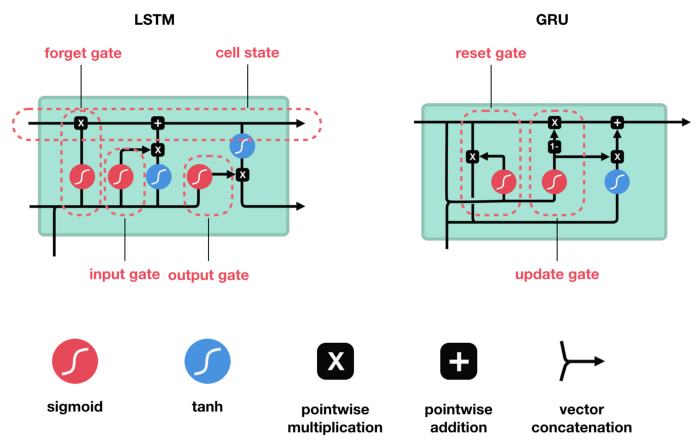
\includegraphics[width=\textwidth]{LSTMvGRU.png}
    \caption{Schematic comparison of LSTMs and GRUs, created by Micheal Phi \cite{phiIllustratedGuideLSTM2020}}
    \label{fig:LSTMvGRU}
\end{figure}

% RNN
% new cell state = tanh(input + previous cell state)

% LSTM
% new cell state = (previous cell state * forget gate) + input gate
% new hidden state = output gate * tanh(new cell state)
% gates:
% \begin{itemize}
%   \item forget gate: sigmoid(input + previous hidden state)
%   \item input gate: sigmoid(input + previous hidden state) * tanh(input + previous hidden state)
%   \item output gate: sigmoid(input + previous hidden state)
% \end{itemize}

% GRU
% new cell state = (previous cell state * update gate) + output gate
% gates:
% \begin{itemize}
%   \item reset gate: sigmoid(input + previous cell state) * previous cell state
%   \item update gate: 1 - sigmoid(input + previous cell state)
%   \item ''output gate'': tanh(input + reset gate) * sigmoid(input + previous cell state)
% \end{itemize}

\subsection{Conditional Recurrent Neural Network}
\label{sec:condRNN}

This is where the conditional recurrent neural network (condRNN) \cite{remyPhilipperemyCondRnn2020} comes in.
Compared to the earlier explained RNN architectures, it allows a second input, a non-sequential input, called conditional input, in addition to the sequential input.
Just what we need for our flow data.
The conditional input gets used to set the initial state of the RNN for each datapoint.
% explain how the initial state is set? not needed I guess
This allows the conditional data to be taken into account without appending it to each timestamp in the sequence.
% TODO
Also see \ref{sec:imagedesc} Image Description Generation in Related Work.

\begin{figure}
    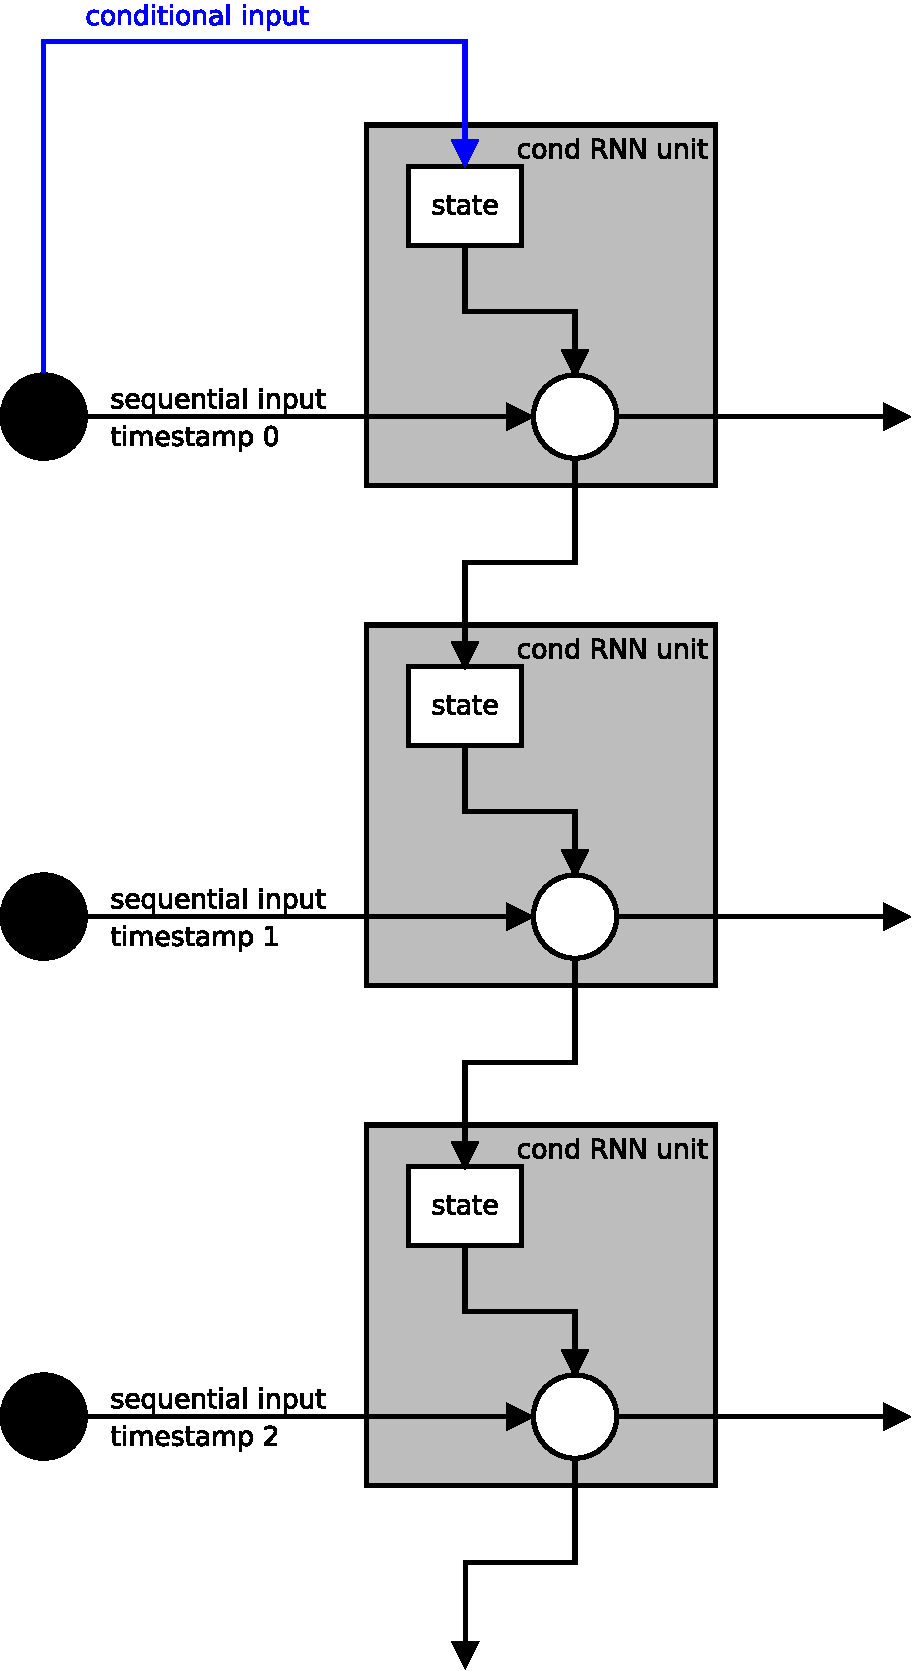
\includegraphics[width=0.6\textwidth]{condRNN.pdf}
    \caption{Schematic sketch of the input for a condRNN unit over time, the areas marked blue present the difference to the normal RNN architecture.}
    \label{fig:condRNN}
\end{figure}

\section{Masking}

The problem presented in this thesis involves the classification of network packets related to their flows.
As network flows vary in sequence length and different protocols contain a different amount of header fields and therefore features, one problem to solve is the inconsitency of our data sequence.
Masking is a common practice in the field of NN models to process sequences with missing data.
The missing data gets filled with a unique value before it is processed by the NN.
This value is called masking value and should not appear anywhere else in the data.
Once the completed sequence is fed into the NN, a masking capable layer processes the input data and creates a vector containing only ones and zeros (or true and false).
This vector is called the mask.
The mask is passed as a separate input to a mask supporting layer of the NN that should process the original input.
The layer processing the input data now can refer to the mask and only takes into account the data that is marked as valid in the provided mask.
% TODO: wording
With this procedure holes in sequence can be closed and sequences of non-uniform length can be padded without changing the requirements for the model. %only because the data is not complete.

\section{GANs}
\label{sec:GAN}

To create a NN that could later be used as a DN we first need to understand how a GAN operates.
A GAN consists of two NNs that compete against each other to maximize the quality of the generated data:
a generator network (GN) and a discriminative network (DN).
The GN creates synthetic samples and the DN gets real or synthetic samples at random.
The DN then needs to decide if the sample it just saw is real or fake.
Afterward, the decisions of the DN gets evaluated and both the DN and GN get fine-tuned based on the results.
% TODO: is this really loss? read the paper
If the decision of the DN was correct than the GN is not good enough too fool the DN and therefore gets a greater loss, while the DN gets a smaller loss.
If the DN was not able to make correct decisions it gets a greater loss and the DN a smaller loss.
The GN is constantly trying to fool the DN with data it generates synthetically,
while is constantly trying to figure out if the data it was given is real or synthetic.
If correctly optimized, a GAN may create synthetic data indistinguishable from real data.

\pagebreak

\section{Terminology}
\label{sec:terminology}

During this work we will use certain phrases and wording that may seem vague but simplifies more complex expressions.

When we say \textit{a sequence of (network) packets belongs to a (network) flow}, we mean that \textit{the (network) flow could have been created from this sequence of (network) packets}.

A \textit{network flow} might also be called \textit{network packet flow}, \textit{packet flow} or just \textit{flow}.

A \textit{network packet capture} might be called \textit{network capture}, \textit{packet capture}, or even \textit{pcap (file)}.

% A \textit{datapoint} within a dataset

When we talk about positive or negative \textit{samples}, the sample means datapoint.

When we talk about \textit{errors} in regards to datapoints, we refer to the alterations made to a positive datapoint so that it becomes a negative datapoint.

A \textit{dead feature} is a feature, which is not properly taken into account by a NN during the learning process, for example because it never changes. In other words, such a feature gets ignored.

\chapter{Related Work}
\label{sec:relatedWork}

% FIXME: add intro
% alt: move intro from related NN models up and rewrite it to fit

\section{Flow-based Network Traffic Generation using Generative Adversarial Networks}
\label{sec:ringGAN}

Ring et al. \cite{ringFlowbasedNetworkTraffic2019a} introduce a GAN to generate synthetic network flows.
Not only are their synthetically created network flows interesting as the source of input for the proposed GAN in future work,
but their choice and classification of network flow features might be a valuable resource for this thesis.
% TODO: explain more?
They classify transport protocol, IP addresses, and ports as categorical features, duration as continuous, the number of bytes, and packets as numeric.
TCP Flags could either by seen as binary attributes or one categorical value.
Even though Ring et al. \cite{ringFlowbasedNetworkTraffic2019a} do not create network packet captures, most of their classification is applicable to our problem.
In addition, they reference and apply a novel approach for the conversion of categorical features of network flows.
They call it IP2Vec.

\subsection{IP2Vec}
\label{sec:IP2Vec}

Network flows consist of multiple features, some of which are categorical, e.g. IP addresses, ports, and protocols.
However, NNs work best with continuous and numerical data.
To effectively train a NNs, which work bast with numerical and continuous data, we need to represent those categorical features as numerical data.
For this we planned on using IP2Vec proposed by Ring et al. \cite{ringIP2VecLearningSimilarities2017}.
This solution produces similarity values for IP addresses based on the behavior of the host.

They based their work on the concept of word2Vec from the field of natural language processing.
There the word is observed in the context of its neighbors instead of alone.
Similarly, in IP2Vec IPs are not observed on their own, but on in the context of other features of the flow, they correlate with.
So instead of words IP2Vec processes network flow attributes,
specifically source IP, destination IP, destination port and protocol.
However one could change those attributes and determine the difference between IPs based on different attributes.
With this approach they are able to determine the differences between IPs based on their communication patterns and behavior within one dataset.
For example, a destination IP that correlates with port 80 often can be easily classified as an HTTP server.
Their experiments show that provided the right dataset, the data produced by IP2Vec can be used to distinguish between infected and non-infected hosts, as well as between servers, clients and even printers.

\subsubsection{Conclusion on IP2Vec}
\label{sec:conclusionIP2Vec}

% We had planned to adapt the IP2Vec approach and extend it to handle not only flow attributes but all packet header attributes.
% However since this approach seems fundamentally flawed.

% used IP2Vec to generate source IP based vectors that represent the similarity between IP addresses within a dataset.

% Out of the YAF flow features the following are used by IP2Vec:
% Duration, protocol, source IP, source port, destination IP, destination port, packet count (forward), octet/byte count (forward)

After due consideration however, we decided not to use the IP2Vec approach.
This is mainly because of the fact that addresses do not influence the flow behavior too much.
The only feature of them that might influence a flow is if they are public or local (private).
Additionally, IP2Vec sees IPs in the context of a series of packet flows, which represent a network traffic capture,
meaning that it relates the IPs to one another depending on the behavior of their flows within one network capture.

This does not apply in our use case, since we use the traffic of multiple network packet capture datasets.
To use IP2Vec we would either have to apply it before extracting the flows and mixing the results,
or mix the flows and then apply IP2Vec to it.
The former has the problem that we would risk introducing false correlations between IPs from different datasets.
As an IP address could appear in more than one network capture and have a completely different behavior in each.
Mixing the information IP2Vec extracted from both of the captures would distort the results of the NN regarding the affected flows.
The later IP2Vec approach has the problem, that IPs will correlate to each other without ever having been in the same network.
IP2Vec does not account for problems that might result from this.
The best-case scenario is that two IPs from different captures will be classified as being unknown to each other.
But even this holds the issue that a later flow may have communication between those IP addresses and the GAN will have problems generating packet data that will satisfy the DN, because to the DN this will look like an anomaly.

Furthermore we would assume that for our GAN in the future work, we have a whole set of flows for each IP address, that could provide the data necessary to apply IP2Vec before using the flow as input to the DN.
This will most likely not be the case, as the GN of the GAN would try to create a sequence of packets based on the input of one flow.
So it would not have the sufficient data to create IP2Vec vectors.
% is this really the problem? I think so
Since both possible approaches have the problem with IPs that might be present in multiple source datasets,
and we can not assume that the future work GAN is able to produce IP2Vec vectors from one flow,
we concluded that IP2Vec is not suitable for our problem.

\section{Related Neural Network Models}
\label{sec:relatedNNmodels}

We researched related work regarding the generation of synthetic network traffic using NN.
But besides Ring et al. there was nothing of interest to this thesis.
However, we also researched RNNs and GANs.
Since some approaches to solutions for other problems might be applicable to our problem of
the discrimination if a network flow could have been created from a given sequence of network packets.
In addition to a GAN utilizing federated learning (FL) by by Rasouli et al. \cite{rasouliFedGANFederatedGenerative2020} that could be interesting to the future work GAN, we found an interesting concept for a RNN.
Once the feature sets of network flows and packets were defined it became clearer which papers where to be considered.
This is when we found Vinyals \cite{vinyalsShowTellNeural2015} and Karpathy \cite{karpathyDeepVisualSemanticAlignments2015} works on image description generation.

% Approaches to generate synthetic network packets that did not use NNs are not really related work,
% since they will not face the same problems as this thesis, therefore they were omitted.

% Bidirectional RNN?

\subsection{Image Description Generation}
\label{sec:imagedesc}

On first glance the field of image description may look out of the scope of this thesis.
However in computer science and machine learning in particular, it is not unlikely for two very separate problems to have the same solution.
The process of teaching a NN to describe an image or even different regions of the image using natural language is a big and complex problem.
The papers "Show and Tell: A Neural Image Caption Generator" by Vinyals et al. \cite{vinyalsShowTellNeural2015} and "Deep Visual-Semantic Alignments for Generating Image Descriptions" by Karpathy and Fei-Fei \cite{karpathyDeepVisualSemanticAlignments2015} both solve this problem in 2015.
However the problem we were interested in is much smaller.

How did both Vinyals and Karpathy solve the problem of multiple inputs for RNNs?
They had the image data and the descriptions in natural language.
While the sequence of descriptions is sequential the image data is not, but it still needed to be included as input for the RNN.
This is where both parties simultaneously create a condRNN, that took the image as conditional input in the beginning and the descriptions as sequential input.
The conditional input conditions the state of the RNN before the sequence is read.
For more details on condRNNs, see also section \ref{sec:condRNN}.

\subsubsection{Deep Visual-Semantic Alignments for Generating Image Descriptions} % Karpathy
\label{sec:karpathy}

Karpathy et al. extract pixel data of the whole image and the 19 locations within the image.
%, extracted by their region convolutional neural network (RCNN).
They use a convolutional neural network (CNN) to convert each set of pixels into a vector of h dimensions.
%, where h is the number of inputs of the RNN.
So each image is represented by a set of 20 vectors with $h$ dimensions.
They use a bidirectional recurrent neural network (BRNN) that takes a sequence of $N$ words and transforms each word again into an $h$-dimensional vector.
This vector got adjusted with 300-dimensional word2vec weights based on its context within the sentence.
They then condition their RNN on the first step with the image date via bias interactions.
Then the RNN processes the sequence of word vectors in order to learn how to predict the next word in the description based on the image data and previous words.
% START AND STOP word

\subsubsection{Show and Tell: A Neural Image Caption Generator} % Vinyals
\label{sec:vinyals}

% TODO: more
Vinyals et al. also use a CNN to create a proper representation of the image that can be passed to the RNN.
For the RNN they chose the LSTM model

\chapter{Methodology}
\label{sec:approach}
\label{sec:methodology}

For our NN model, we assume that some form of Recurrent Neural Network (RNN) will be suitable as a discriminator of a GAN that can create synthetic network packet captures from network flows.
Since simpleRNNs have the problem of short-term memory, we propose the use of either Long Short Term Memory (LSTM) networks \cite{hochreiterLongShortTermMemory1997} or Gated Recurrent Units (GRUs) \cite{bahdanauNeuralMachineTranslation2016}.
GRUs tend to use fewer operations and states to produce similar or better results than LSTMs.
But depending on the use case, LSTMs might still produce better results.
It is to be determined, which of the two neural networks provides better results for the problem in this thesis.

For this we will run experiments with the \textbf{simpleRNN}, \textbf{LSTM} and \textbf{GRU} layers provided in Tensorflow.
\textbf{simpleRNN} will provide the baseline for the real contenders \textbf{LSTM} and \textbf{GRU} during the experiments, as it will most likely provide the least optimal results.
Before we can pursue the experiments however we need data to train and test with.

\section{Dataset}
\label{sec:dataset}

For our dataset, we will extract packet sequences and corresponding network flow from publicly available and well-known network packet captures and create network flows based on these sequences.
Each network packet sequence will be paired with its network flow so that our NN can learn the connection between the two data structures.
Since the end goal in the future work GAN is to generate the complete packet sequences based of the flows,
each sequence of packet features will contain as much of the original header information as needed to reconstruct a packet sequence from them.
This way, no crucial information gets lost and the DN is prepared to handle the complete data of a packet capture, compare them to flows and make an informed decision if a network flow belongs to a packet sequence.

Each flow attribute and packet header field is converted into an appropriate representation depending on its data type and meaning for the sequence of packets.
Since the NNs are most efficient with continuous and numerical data, we will convert all fields accordingly, wherever possible.
We will also implement a pipeline to create negative samples from the ground truth, which builds our positive samples.
% Both will be discussed further in the dataset preprocessing section.

\subsection{Dataset Preparation}
\label{sec:datasetPrep}

The NN needs to be trained with a significant amount of both positive and negative datapoints so that it can make informed decisions.
First, we collect samples that represent the ground truth and will be our positive datapoints.
We sample flows from multiple packet captures we extracted from popular intrusion detection datasets with network traffic packets.
Then to create negative datapoints, we randomly apply modifications to the previously collected positive samples.

\subsubsection{Sampling}
\label{sec:sampling}

Instead of collecting all flows from our source captures, we sample sequences of packets from only one packet capture of each dataset.
This may not seem like much but as we only plan on creating a small proof of concept the data should be sufficient.
The sampled packet sequences and flows are stored separately as csv files for further preprocessing, as network packet captures are usually slow to process.
For our purpose, we considered two approaches for sampling a network packet capture for flows.
Either by sampling through the packet sequences within the captures or by splitting the capture into intervals and sampling through those partial captures.
Splitting the capture into intervals is less compute-heavy and therefore less time-intensive since the resulting packet captures are smaller and much quicker to parse.
Although this might truncate some flows, it should not be a problem, since a capture itself is truncated at the beginning and end anyway
and we also use timeouts (20 seconds) for the flow collecting, which will truncate the flows once again.
Additionally, we do not require flows longer than the intervals themselves,
as we want to keep our packet sequences short enough to be reasonably processed by an RNN.
Later during the further preprocessing, we drop any flow longer than a maximum number packets (500), to ensure an equal length for all our packet sequences.

The question however is the length of the intervals.
Should they be determined relative to the size of the capture or should they have a fixed length?
A fixed-length may provide better comparability between the flows across different captures,
but the variation between packet captures regarding packet rate (frequency) may proof to be problematic.
As setting the fixed length to low may yield the problem that some captures return empty intervals
and setting it too high might result in too large intervals and therefore in less efficiently parsable partial captures.
An interval length based on the percentage of each individual capture does not have those faults.
Even though it might shrink the flow duration of smaller captures, it appears to be the better approach.
In addition, extracting packet sequences with a relative offset within a capture might provide sequences with a wider range of flow behavior.
Now that we know we want to split the capture first, it is to be decided, how we sample the packet sequences within an interval.
We can make an educated guess that randomly selected samples will yield better results than sequential sampling, as it again provides a wider range of flow behavior.

So for our dataset, we decided that splitting the capture into intervals first would be the right approach.
We split the captures into intervals relative to its size.
This way we will preserve the behavior of the sampled flows within the larger network within each specific interval.
Afterward, we will randomly sample up to 250 of TCP and UDP packet sequences alike within those intervals.
Please note not all source files provide enough flows per-protocol though, specifically UDP packets seem to be less prominent.
Each sampled packet sequence will be exported as a capture first using Wireshark's \code{editcap}.
The header fields of the packets belonging to the sequence will be stored as a csv file for easier parsing, exported by Wireshark's \code{tshark}.
Then we use YAF to extract the flow information and \code{yafscii} to create flow-based csv files form the exported capture.

\subsubsection{A Padding supported Conversion from UDP to TCP}
\label{sec:UDPpadding}

Each datapoint in our dataset can either be a TCP or a UDP packet sequence.
Compared to UDP packets, TCP packets have more header fields and therefore more features get derived from TCP packets compared to UDP packets.
% FIXME: wording
This results in an uneven timestamp size or length of packet data between two datapoints, if one is based on a UDP packet and the other is a TCP packet.
To make packets of both protocols comparable, we will add padding to the UDP packets.
We add the TCP flags and options as well as the sequence number and window size at the same positions where they would be in a TCP feature vector, more on that in section \ref{sec:packtFeatures}.
% FIXME: wording
They get assigned our padding value (-15), which will be used as a masking value during the input into the NN.
To round it up we convert the UDP length to TCP header length and TCP payload length, see section \ref{sec:packtFeatures} paragraph \textbf{derivation}.
The last part is especially important to keep the datapoints comparable and not only at the same length.
This way, the NN can make the right decisions based on the data and is not held back by matching single features between the two protocols.
% FIXME: maybe add packet padding subsection, but it is more a NN input thing than a dataset thing right?
As our positive datapoints are ready for processing now, all that is left to do to complete our dataset is the creation of the negative samples.

\subsubsection{Creation of negative samples}
\label{sec:negativeSamples}

To create negative samples we use four different methods.
The selection of ground truth samples that will be falsified is randomized in all methods.
The first method is \textbf{altering packet and flow features} by either sampling features \textbf{from another datapoint} of the dataset (\textbf{method 1b}) or generating \textbf{random values} (\textbf{method 1a}), which lie within a rough frame of expectation for the feature.
For the frame of expectation, we used the number of bits available to the header fields, as they provide the hard limit to the range of the feature's value.
\textbf{Method 1} is able to produce three different types of negative samples:

\begin{itemize}
    \item a datapoint, which has altered packets
    \item a datapoint, which has a altered flow
    \item a datapoint, which has both altered
\end{itemize}

Please note that we later decided not to alter the flow as the RNN should learn if a packet sequence could have been created by a given flow and also detecting altered flows would lead the classifier to learn unnecessary information.
Furthermore in the scenario of our future GAN, the flow input is authentic and does not need to be classified itself for authenticity.
However dropping altered flows did not change the performance of our model, so the model would likely perform the same through the later experiments if the altered flows were present in our dataset.

The second method is randomizing the \textbf{packet order} (\textbf{method 2}) within the packet sequence of a given datapoint.
The third is to \textbf{decrease} or \textbf{increase} the number of packets of the sequence in a given datapoint (\textbf{method 3}).
To decrease the number of packets we just remove a random number of packets at a random position.
To increase the number of packets we again sample from another datapoint in the dataset and add some of its packets to the current sequence.
And the fourth and final method is \textbf{mismatching} network flows with a different sequence of packets (\textbf{method 4}).

Each negative sample creation method has one or more parameters, which decide the degree to which it alters the ground truth sample.
% it extracts its data from, a positive datapoint from the dataset.
The degree of \textbf{method 1} is defined by the number of errors assigned to every packet and the number of altered packets.
The degree of \textbf{method 3} is defined by the number of packets added to or removed from the sequence.
While adding packets was done by a total amount, removing packets was done relative to the sequence size, as having a lot of negative samples with sequences of small size might cause the NN to learn that small sequences are per default negative.
The \textbf{methods 2 and 4} have no degree, they are completely random and have no parameters adjusting the severity of the error.

The parameters used to change the degrees stay not completely static either.
We randomize them within a given range that seemed appropriate to the parameter.
For example, adding packets using \textbf{method 3} adds $+/-10$ packets, so using the parameter $0$ packets equals adding $1$ to $10$ packets at random, while using the parameter $15$ would add between $5$ and $25$ packets.
\textbf{Method 1} uses a range of $+/-5$ for the number of errors per packet.
Initially, the number of packets altered was a static one, but later we did the same $+/-5$ range for the numbers of altered packets, for the creation of the \textbf{20 packets} dataset, see section \ref{sec:datasetStats}.

Using different methods to create negative datapoints provides us with a good mix of negative datapoints.
This is important in order to effectively train the NN, as it will face many different errors in packet sequences in a real-world application.
However, it is important to falsify the data realistically, so that the NN is efficiently tested for future use within a GAN.
For this, we need to provide a good representation of each feature from packets and flows alike.

\subsection{Datapoint Features}
\label{sec:datapointFeatures}

In this section we discuss, which features will be part of our dataset and how they need to be derived, so that they could be used as input for the NN.
% FIXME: move this UP? to where?
We will generally focus only on IPv4 traffic to keep it simple.
Also, we will focus on the TCP and UDP protocols for now.
All network traffic features influencing network flow behavior will be of importance to our NN.
This property will therefore decide the datapoint features.
Network flow attributes and sequences of packet header fields will be the source for our datapoints.

% Network flows created by YAF contain the following features:
% % start-time, end-time, duration, rtt, proto, sip, sp, dip, dp, iflags, uflags, riflags, ruflags, isn, risn, tag, rtag, pkt, oct, rpkt, roct, end-reason
% Timestamps for start and end time, duration, round trip time, protocol, source IP, source port, destination IP, destination port, TCP flags (forward and reverse), initial TCP sequence number (forward and reverse), first-packet 802.1q VLAN tag (forward and reverse), packet count (forward and reverse), octet/byte count (forward and reverse), the reason for the end of the packet sequence.

\subsubsection{Packet sequence features}
\label{sec:packtFeatures}

\definecolor{not}{HTML}{949698} % Gray
\definecolor{trivial}{HTML}{ed1b23} % Red
\definecolor{derivation}{HTML}{fff200} % Yellow
\definecolor{feature}{HTML}{41b0e4} % CornflowerBlue
\definecolor{dropped}{HTML}{99479b} % purple

Each packet contains a variety of header fields depending on its protocol, the position within a communication stream, and the options chosen by the communicating endpoints.
It is to be decided, which of those header fields are of importance to our goals.
If we just wanted to validate that a sequence of packets belongs to a flow, we could argue that the only header fields interesting are the ones that are present in the flow representation as well.
But for the future work GAN, this would not be enough.
Instead, we want our NN to learn the correlation between all packet header fields and the limited flow features.
This will enable the NN to be used as a DN for the proposed GAN later.
One could argue that to properly correlate between flows and packets we need all of the header fields of each packet.
%Ideally all of them, but some can be ignored and others simplified for the NN.
However, most of the header fields can be trivially verified by means of direct comparison to the flow features (e.g. addresses), order checking (e.g. acknowledgement numbers) or similar methods.
% FIXME: wording
For this reason, some header fields are insubstantial for our use case for example, the addresses of the communicating endpoints (source and destination).
This would include MAC and IP addresses for example.

Neither extreme would be the right approach.
Instead, we suggest sorting the packet header fields and flow attributes into the following different categories:
\colorbox{not}{\textbf{{Not Used}} (gray)},
useful but \colorbox{trivial}{\textbf{Trivial} (red)},
\colorbox{dropped}{\textbf{Dropped} (purple)},
\colorbox{derivation}{\textbf{Feature Derivations} (yellow)},
and raw \colorbox{feature}{\textbf{Features} (blue)}.
We color-coded the five categories in order to give a more direct overview of membership for the packet header fields in tables \ref{mac} to \ref{udp} present.
In the following paragraphs we briefly explain the meaning of each category and explain the membership of packet header fields.

\paragraph{\colorbox{not}{\textbf{{Not Used} (gray)}}} are header fields that do not change ever or at least not in our scenario.
This includes the Version of the IP Header since we only take IPv4 traffic into account,
and the reserved bits in the IP flags and the TCP header.

\paragraph{\colorbox{trivial}{\textbf{Trivial} (red)}} header fields might be useful, but should not be fed to the NN.
Either because they can easily be validated outside the NN and might slow the NN down for no benefit,
or they do not alter the behavior of the network flow.
% QUESTION: what about IP class? this could be an interesting feature
% No, but difference between public and local.
This would include header lengths, urgent pointer, as well as MAC and IP addresses.
% FIXME: header lengths
The acknowledgement number order can be easily checked outside the NN and can be omitted as well.

\paragraph{\colorbox{dropped}{\textbf{Dropped} (purple)}} fields could have been \colorbox{derivation}{\textbf{Feature Derivations} (yellow)}, but were omitted due to a lack of data.
A NN needs a large amount of data to make proper decisions, if the data is not sufficient and it encounters a feature for the first time it would at best classify the datapoint correctly with a 50\% chance.
The best case of insufficient data is no data, so the NN would ignore the feature, but as such features would just be a \textbf{dead feature}, it is better still to omit it.
For IP options and the TCP flag NS, also called the ECN-nonce, the data is inconclusive,
as our dataset does not contain any flows with IP options and only three with an ECN-nonce.
This however is not unusual, as those fields are rarely used in practice anyway.
Our dataset supports our research results that this is indeed just normal network traffic behavior,
since it is constructed from numerous network packet captures from statistically different intrusion detection datasets.
Luckily network flows do not contain either of those header fields in their attributes, meaning it should not impact our results to omit the two.
IP options would influence the behavior of a flow, but as our dataset does not contain any IP options, omitting them should not result in bad training results.
It only means that in order to take IP options into account in the future our NN and preprocessing needs to be expanded.
However, most of the implementation was already done and could be easily adjusted to fit this need.
The ECN-nonce is the more acute problem since less than 0.0009\% of datapoints use it,
which would add risk for our NN to misinterpret the data, once it comes across such a datapoint.
Omitting the ECN-nonce should not be a problem either, as the feature does not impact the behavior of the flow in any way that is not already indicated by the ECN flag and value, see later in this section.

\paragraph{\colorbox{derivation}{\textbf{Feature Derivations} (yellow)}} are fields, which are important to our probkem, but can not be used as direct input to the NN.
They need to be \textbf{derived} in some way beforehand.
The raw data representation of those features is not optimal as NN input and needs to be abstracted first.
The most prominent type of feature with this property is the categorical feature, but simple byte or string conversion can also already qualify for this category of header fields.
The type of derivation can vary from header field to header field.
The protocol for example can be represented as a single boolean as our dataset only contains TCP and UDP, where 1 stands for TCP and 0 for UDP.
Take note that UDP length, which describes the total length of the UDP frame, will be derived to fit the TCP length fields.
It is simple split into \code{tcp.len}, a Wireshark filter describing the payload size of TCP packets, and the data offset, which is equivalent to the TCP header length.
This way packets of the two different protocols are comparable.

The checksums are a perfect example for a feature derivation that can be abstracted quite a bit.
It does not matter to the NN what the checksum reads as the future work GAN should not have to generate checksums at all.
It should generate the header fields that change the behavior of the flow.
The checksum for the packets of the output sequence could be easily generated after the generation of the header fields and therefore outside the GAN.
%The actual checksum could be easily calculated after those fields have been generated by the GAN.
But an invalid checksum may influence the flow of packets, in the sense that the packet might get requested again and will be resend.
So for our DN it only matters if the checksum matches the header.
% The same would go for the header length if it would not provide the offset information for IP and TCP options.
% as well as the difference for the payload. % not needed
So instead of feeding the NN the raw checksum and therefore teaching it how checksums work, we will provide its status in regards to validity with a simple boolean.

The ports are categorical features and need to be converted to a continuous data representation.
This is done by sorting the port into the following categories based on port ranges defined by the IANA \cite{ServiceNameTransport}:
% \textbf{system} ports (0-1023), \textbf{registered} or user ports (1024-49151) and \textbf{ephemeral} or dynamic ports (49152-65535) \cite{ServiceNameTransport}.
\begin{itemize}
    \item \textbf{system} ports (0-1023)
    \item \textbf{registered} or user ports (1024-49151)
    \item \textbf{ephemeral} or dynamic ports (49152-65535)
\end{itemize}
Additionally the ephemeral category is split into the following subcategories:
\begin{itemize}
    \item \textbf{IANA} (49152-65535): the range of ports assigned as dynamic by the Internet Assigned Numbers Authority (IANA) \cite{ServiceNameTransport}
    \item \textbf{linux} (32768-60999): ephemeral ports accessable on linux based systems through \code{/proc/sys/net/ipv4/ip\_local\_port\_range}
    \item \textbf{bsdold} (1024-5000): ephemeral ports used by older (Free)BSD implementations (version < 4.6) \cite{EphemeralPortRange}
    \item \textbf{winserver} (1025–65535): dynamic ports used by Windows Server 2000 \cite{DefaultDynamicPort} \cite{WhenYouTry}
    \item \textbf{winxp} (1025–5000): dynamic ports used by Windows XP \cite{CableGuyDecember} and Server 2003 (until update MS08-037) \cite{YouExperienceIssues}
\end{itemize}
Newer versions of Windows use the IANA range \cite{DefaultDynamicPort}, so the we can spare a new feature for it.
Only Windows Server 2008 with Exchange Server 2007 uses 1025–60000, which is still within the \textbf{winserver} category \cite{DefaultDynamicPort}.
In future work one could expand this binary representation by adding subcategories to the system and registered ports.
But this is out of the scope of this thesis.

It is important that we derivate TCP options to remove dead features and preserve the information that is important to our problem,
as TCP options such as maximum segment size (MSS) and selective acknowledgment (SACK) may impact a network flows behavior,
while others may never occur, just like the IP options described above.
We collect the MSS, SACK and the timestamp options,
as they are the most prominent and frequent options used and
our dataset also does not contain any other TCP options.
The timestamps get converted to the relative timestamp based on the earliest timestamp in the packet sequence in order to compare them to the \code{frame.time\_relative} filter option from Wireshark.

The Explicit Congestion Notification (ECN) \cite{floydAdditionExplicitCongestion} header field has a simple derivation, although an important one.
It consists of two bits that are interpreted as an integer by Wireshark.
However, the bits are a categorical feature comparable with the IP and TCP Flags.
If neither bit is set, ECN is not supported by the sender.
If either one bit is set by itself, ECN is supported by the sender.
If both bits are set, there is network congestion on the route between the sender and the receiver.
This leaves us with two boolean features as input for our NN: ECN capable transport and congestion encountered.
If we look into the documentation of ECN, we will see that those are the only attributes the ECN provides \cite{DifferentiatedServicesField} and our derivation in fact matches the information ECN supporting hard- and software extracts from the header fields.
% TODO: explain categorical feature abstraction. is this still needed?

The Differentiated Services Code Point (DSCP), formerly Type of Service (ToS), header field has a more complicated derivation.
Its specification is open for experimental and future standard values.
For this reason, it is divided into 3 pools of values, specified by the values last two bits \cite{DifferentiatedServicesField}.
The first pool (xxxxx0) contains standard codepoints and still unassigned values, reserved for later standards.
The second pool (xxxx11) is reserved for local use or experimental codepoints.
The third pool (xxxx01) contains codepoints for local use or experimental, but will be used for standard codepoints once the first pool is exhausted.
We abstract this behavior with two features: local (or experimental) and standard.
This allows us to keep the parameters for the pool category minimal.
But the pools are not the only scheme by which DSCPs are categorized.
There are five major categories of standardized DSCPs, of which two have ranked subcategories.
The five categories \textbf{Low Effort} \cite{blessLowerEffortPerHopBehavior}, \textbf{Class Selector (CS)} \cite{nicholsDefinitionDifferentiatedServices}, \textbf{Assured Forwarding (AF)} \cite{wroclawskiAssuredForwardingPHB}, \textbf{Voice Admit} \cite{bakerDifferentiatedServicesCode}, and \textbf{Expedited Forwarding} \cite{firoiuExpeditedForwardingPHB} will again be used as boolean features for the NN input.
This way we complete the binary representation of DSCPs.
However, CS and AF are again ranked within their category.
Both have an IP precedence class, which is ranked from 1 to 7, where packets of class 7 have the highest priority, and packets with class 1 have the lowest.
AF only allows the first four classes (1-4) though.
% higher relative order (in the queue?)
AF also has the drop precedence probability, which is ranked "Low", "Medium", and "High", or in our abstraction 1 to 3, and is used within one class, so to not overwrite the priority set by the IP precedence, but to rank within one such class.
As the name suggests the higher the precedence probability class the more likely the packet is dropped, so here the higher number has the least priority.
% Two solutions: one hot or integer % which?
Both of these classifications will be represented as an integer value.

\paragraph{\colorbox{feature}{\textbf{Features} (blue)}} are fields that we can use as unmodified or raw input.
They are numerical (integer, float) or truth based (boolean) and can therefore be interpreted by a NN.
But not all numerical or boolean fields automatically qualify as features.
For example the transport protocol is represented as a numerical value, but it would be ineffective to train a NN based on that number.
It would try to perform operations on it like on any integer value, but that would lead to wrong results.
In the best case it would to no result, while creating overhead during computation.
The fields qualifying for this category need to be continuous data.
Additionally to the packet header fields shown in the table we also considered some meta data.
As mentioned before we use the relative time offset of the packets, this feature should match with the duration of the flow,
and the TCP payload length, provided by Wireshark's filter \code{tcp.len}.

The identification IP header field uniquely identifies a network packet compared to other packets from the same source.
As it is just counting up, one could suggest, that it is not more of a feature than the acknowledgment number.
However in a network packet capture it is possible that a source's packets are not monitored continuously, for example behind a NAT,
thus their intermediate packets would not be recorded.
This would require a more sophisticated approach for generating IDs for synthetic packets.
Therefore we suggest letting the future GAN learn to create such an ID itself in this case, our NN needs to learn the relationship between those IDs too.

The IP and TCP flags are already in binary representation and can be fed to the NN as is.
The TCP flags are of more importance than the IP flags though, as our flow representation also includes them.
% FIXME: wording and maybe explain what "important" means
As fragment offset, the time to live (TTL) value and the window size are as important to flow behavior as the flags and are all numerical, we include them as features as well.
% maybe trivial after all? maybe, but not for this thesis
The sequence number could just as easily be compared to the initial sequence number contained in the flow data.
However, the position of the sequence number in the packet sequence can decide if a flow is valid or not.

% UDP length will be derived as data offset and length from TCP
% FIXME: wording
% The data offset and IP header length (IHL) are also used as an indicating boolean for TCP and IP options respectively.
The data offset and IP header length (IHL) are indicating that TCP and IP options should be present, this provides interesting context between packet (header) length and other features.
Combined with the total length it also gives us information about the payload size.
As the UDP length will have been converted to TCP length and data offset, packets of both protocols will benefit from this.
Now that we know the network packet features and their derivations, we need to apply the same principles to network flows, the counterpart to a packet sequence.

\subsubsection{Network flow features}
\label{sec:flowFeatures}

Network flow features will be classified in the same categories as the packet header fields.
Table \ref{flow} shows the color-coded flow features.
In this work, we need to abstract flow behavior from a sequence of packets and compare it to the features of a given flow.
As a flow has a higher abstraction from network traffic than packets, we can omit less features.
Please note however that the reverse features, which a YAF flow representation provides, will be omitted anyway due to the fact that it does not relate to the packet sequence of the flow, but to the counter part of it.
Meaning the flow from destination to source.

IP addresses and timestamps might mislead our classifier, as a flow might have almost the same behavior even though it has two different endpoints communicating or was sent at another time.
As mentioned in the previous section (IP) addresses can be easily compared outside of the NN and are therefore \colorbox{trivial}{\textbf{trivial} (red)}.
The same applies to the timestamps.
Although timestamps have an additional problem. As they are large floating-point numbers, they might slow the NN down.

Duration, round trip time, as well as packet, and byte count are already present as numerical continuous data, therefore, they can be used as raw \colorbox{feature}{\textbf{features} (blue)}. The initial sequence number falls under the same category just as their header field counterpart did.

The rest of the features are to be \colorbox{derivation}{\textbf{feature derivations} (yellow)} and will be derived in a way that fits the derivations of their packet field counterparts.
The protocol and ports are derived the same way the packet derivations did it.
A YAF flow contains the TCP flags of the first and last packet of the sequence of packets is was created from.
The flags are provided as strings by yaf containing the initial letter of each active flag:
\textbf{F}IN, \textbf{S}YN, \textbf{R}ST, \textbf{P}SH, \textbf{A}CK, \textbf{U}RG, \textbf{E}CE, \textbf{C}WR.
While a \textbf{0} means no flags were active.
To conform with our previous binary representation, we create a boolean for each flag in the same order a TCP packet contains them.
For further details on the derivation of protocol, ports, and TCP flags, see paragraph derivations in section \ref{sec:packtFeatures}.
The end-reason describes the reason for the end of the packet sequence.
It is given as a string and can have five different values:
\begin{itemize}
    \item \textbf{idle} timeout
    \item \textbf{active} timeout
    \item \textbf{eof} interrupted by YAF's timeout or end of file
    \item \textbf{rsrc} premature flush if YAF's flow table maximum is reached
    \item \textbf{force} for single UDP packet flow records that belong to a bigger flow
\end{itemize}
As this is a categorical feature and each end reason mutually excludes all others, we decided to use a one-hot encoding for the binary representation.
Please note that the last two end-reasons do not appear in our dataset, so their derivations are dead features.
This was only discovered after most experiments had already been conducted.
However as stated before, dead features do not effect the results of a NN, but only introduce overhead.
This can be adjusted in the future.

% Later: "data preprocessing"

% FIXME: remove ip2vec
% Additionally IP2Vec extracts the attributes Day and Time from the start timestamp,
% where Day is a boolean representing weekday or weekend
% and Time is the time of day, striped from the date.
% However IP2Vec only uses them temporarely.
% We will extract those attributes from IP2Vecs preprocessing and use them as opposed to the start timestamp,
% since they are more generic, therefore provide better comparability and still ancer the flow to a specific time.
% % TODO: export these features for our NN

% We now need to decide, which other attributes of a network flow are of value to our neural network.
% Since IP2Vec only helps us represent the categorical attributes, there are still bool, numerical and continuous attributes left for us to use.
% We just need to look at their value for the NN.

% After we decided over the flow attributes %(and they work with the NN)
% we might take a closer look at the packet level attributes, a flow does not provide and decide if the extra implementation is worth it.

% TODO: compare single flow from packet capture? or even extract "single flow" packet captures from the whole packet capture

\begin{table}
    \centering
    \begin{tabular}{|r*{32}{|c}|}
        \hline
        bit & 0 & 1 & 2 & 3 & 4 & 5 & 6 & 7 & 8 & 9 & 10 & 11 & 12 & 13 \\
        \hline
        0   & \multicolumn{6}{|c|}{\cellcolor{trivial} Desitnation} & \multicolumn{6}{|c|}{\cellcolor{trivial} Source} & \multicolumn{2}{|c|}{\cellcolor{not} Type} \\
        \hline
    \end{tabular}
    \caption{MAC Header (Ethernet II)}
    \label{mac}
\end{table}

\begin{table}
    \centering
    \begin{tabular}{|r*{32}{|c}|}
        %\hline
        %bit & 0 & 1 & 2 & 3 & 4 & 5 & 6 & 7 & 8 & 9 & 10 & 11 & 12 & 13 & 14 & 15 & 16 & 17 & 18 & 19 & 20 & 21 & 22 & 23 & 24 & 25 & 26 & 27 & 28 & 29 & 30 & 31 \\
        \hline
        %bit & \multicolumn{8}{|l|}{0} & \multicolumn{8}{|l|}{8} & \multicolumn{8}{|l|}{16} & \multicolumn{8}{|l|}{24} \\
        bit & \multicolumn{8}{|l|}{0} & \multicolumn{8}{|l|}{8} & \multicolumn{3}{|l|}{16} & \multicolumn{13}{|l|}{19} \\
        \hline % \multicolumn{3}{|c|}{Flags} % \makecell{E\\C\\N}
        0   & \multicolumn{4}{|c|}{\cellcolor{not} Version} & \multicolumn{4}{|c|}{\cellcolor{feature} IHL} & \multicolumn{6}{|c|}{\cellcolor{derivation} DSCP} & \multicolumn{2}{|c|}{\cellcolor{derivation} ECN} & \multicolumn{16}{|c|}{\cellcolor{feature} Total Length} \\
        \hline % \multicolumn{3}{|c|}{Flags} | \makecell{D\\F} \makecell{M\\F}
        32  & \multicolumn{16}{|c|}{\cellcolor{feature} Identification} & \cellcolor{not} 0 & \cellcolor{feature} DF & \cellcolor{feature} MF & \multicolumn{13}{|c|}{\cellcolor{feature} Fragment Offset} \\
        \hline
        64  & \multicolumn{8}{|c|}{\cellcolor{feature} Time To Live} & \multicolumn{8}{|c|}{\cellcolor{derivation} Protocol} & \multicolumn{16}{|c|}{\cellcolor{derivation} Header Checksum} \\
        \hline
        96  & \multicolumn{32}{|c|}{\cellcolor{trivial} Source IP Address} \\
        \hline
        128 & \multicolumn{32}{|c|}{\cellcolor{trivial} Destination IP Address} \\
        \hline
        160 & \multicolumn{32}{|c|}{\cellcolor{dropped}}\\\cline{1-1}
        192 & \multicolumn{32}{|c|}{\cellcolor{dropped}}\\\cline{1-1}
        224 & \multicolumn{32}{|c|}{\cellcolor{dropped}}\\\cline{1-1}
        256 & \multicolumn{32}{|c|}{\multirow{-4}{*}{\cellcolor{dropped} Options (if IHL > 5)}} \\
        \hline
    \end{tabular}
    \caption{IPv4 Header}
    \label{ip}
\end{table}

\begin{table}
    \centering
    \begin{tabular}{|r*{32}{|c}|} % m{0.2pt}
        \hline
        %bit & 0 & 1 & 2 & 3 & 4 & 5 & 6 & 7 & 8 & 9 & 10 & 11 & 12 & 13 & 14 & 15 & 16 & 17 & 18 & 19 & 20 & 21 & 22 & 23 & 24 & 25 & 26 & 27 & 28 & 29 & 30 & 31 \\
        bit & \multicolumn{4}{|l|}{0} & \multicolumn{3}{|l|}{4} & \multicolumn{9}{|l|}{7} & \multicolumn{16}{|l|}{16} \\
        \hline
        0   & \multicolumn{16}{|c|}{\cellcolor{derivation} Source Port} & \multicolumn{16}{|c|}{\cellcolor{derivation} Desitnation Port} \\
        \hline % \cellcolor{derivation}
        32  & \multicolumn{32}{|c|}{\cellcolor{feature} Sequence Number} \\
        \hline % \cellcolor{derivation}
        64  & \multicolumn{32}{|c|}{\cellcolor{trivial} Acknowledgement Number} \\
        \hline % \makecell{Data \\Offset}
        96  & \multicolumn{4}{|c|}{\cellcolor{feature} Data Offset} & \multicolumn{3}{|c|}{\cellcolor{not} Reserved} & \multicolumn{9}{|c|}{\cellcolor{feature} Flags} & \multicolumn{16}{|c|}{\cellcolor{feature} Window Size} \\
        \hline
        128 & \multicolumn{16}{|c|}{\cellcolor{derivation} Checksum} & \multicolumn{16}{|c|}{\cellcolor{trivial} Urgent Pointer (if URG set)} \\
        \hline
        160 & \multicolumn{32}{|c|}{\cellcolor{derivation}}\\\cline{1-1}
        ... & \multicolumn{32}{|c|}{\multirow{-2}{*}{\cellcolor{derivation} Options (if data offset > 5. Padded at the end with "0" bytes if necessary.)}} \\
        \hline
    \end{tabular}
    \caption{TCP Header}
    \label{tcp}
\end{table}

\begin{table}
    \centering
    \begin{tabular}{*{9}{|c}|}
        \hline
        \cellcolor{dropped} \makecell{N\\S} & \cellcolor{feature} \makecell{C\\W\\R} & \cellcolor{feature} \makecell{E\\C\\E} & \cellcolor{feature} \makecell{U\\R\\G} & \cellcolor{feature} \makecell{A\\C\\K} & \cellcolor{feature} \makecell{P\\S\\H} & \cellcolor{feature} \makecell{R\\S\\T} & \cellcolor{feature} \makecell{S\\Y\\N} & \cellcolor{feature} \makecell{F\\I\\N} \\
        \hline
    \end{tabular}
    \caption{TCP Flags}
    \label{flags}
\end{table}

\begin{table}
    \centering
    \begin{tabular}{|r*{32}{|c}|}
        \hline
        %bit & 0 & 1 & 2 & 3 & 4 & 5 & 6 & 7 & 8 & 9 & 10 & 11 & 12 & 13 & 14 & 15 & 16 & 17 & 18 & 19 & 20 & 21 & 22 & 23 & 24 & 25 & 26 & 27 & 28 & 29 & 30 & 31 \\
        bit & \multicolumn{16}{|l|}{0} & \multicolumn{16}{|l|}{16} \\
        \hline
        0   & \multicolumn{16}{|c|}{\cellcolor{derivation} Source Port} & \multicolumn{16}{|c|}{\cellcolor{derivation} Desitnation Port} \\
        \hline
        32  & \multicolumn{16}{|c|}{\cellcolor{derivation} Length} & \multicolumn{16}{|c|}{\cellcolor{derivation} Checksum} \\
        \hline
    \end{tabular}
    \caption{UDP Header}
    \label{udp}
\end{table}

\begin{table}
    \centering
    \begin{tabular}{|c|}
        \hline
        % FIXME: remove demo stuff, adjust for YAF
        % start-time, end-time, duration, rtt, proto, sip, sp, dip, dp, iflags, uflags, riflags, ruflags, isn, risn, tag, rtag, pkt, oct, rpkt, roct, end-reason
        \cellcolor{trivial} Start Timestamps \\
        \hline
        \cellcolor{trivial} End Timestamps \\
        \hline
        \cellcolor{feature} Duration \\
        \hline
        % OR trivial?
        \cellcolor{feature} round trip time \\
        \hline
        \cellcolor{derivation} protocol \\
        \hline
        \cellcolor{trivial} source IP \\
        \hline
        \cellcolor{derivation} source port \\
        \hline
        \cellcolor{trivial} destination IP \\
        \hline
        \cellcolor{derivation} destination port \\
        \hline
        \cellcolor{derivation} TCP flags (forward only) \\
        \hline
        \cellcolor{feature} initial TCP sequence number (forward only) \\
        \hline
        % TODO: what exactly does this store/return; is it useful?
        \cellcolor{feature} first-packet 802.1q VLAN tag (forward only) \\
        \hline
        \cellcolor{feature} packet count (forward only) \\
        \hline
        \cellcolor{feature} octet/byte count (forward only) \\
        \hline
        % TODO: what exactly does this store/return; is it useful?
        \cellcolor{derivation} the reason for the end of the packet sequence. \\
        \hline
    \end{tabular}
    \caption{YAF IPFIX Template}
    \label{flow}
\end{table}

\subsection{Network Packet Captures used}
\label{sec:pcapsUsed}

For the creation of our datasets, we need network packet captures as sources.
For this, we take a look at publically available intrusion detection datasets.
Since the goal of our future work is to produce network packet captures, that can be used in the field of NID.
As stated above we will extracted data from multiple popular datasets, such as: \textbf{CDX}, \textbf{DARPA}, \textbf{MACCDC}, \textbf{MAWI}, \textbf{Simpleweb}, and \textbf{UNSW}.
% TODO: maybe add a pcap from my personal network
We chose these datasets because of their significant statistical differences, which has been shown in the paper "On generating network traffic datasets with synthetic attacks for intrusion detection" by Cordero et al. \cite{corderoGeneratingNetworkTraffic2019}.
% FIXME: wording
This is important as we need to provide the NN with enough data to distinguish flow behavior in order to match packets to them.
% or so we though

\paragraph{CDX} The data capture from the U.S. National Security Agency (NSA) published in 2009 \cite{CyberResearchCenter}.
% TODO: write some more here
\code{CDX westpoint/2009-04-21-04-06-19.dmp12}

\paragraph{DARPA} The Intrusion Detection Data Sets from 1998 and 1999 \cite{1999DARPAIntrusion}.
This dataset provides PCAP files that were captured in a simulation network.
We chose a training capture that does not contain any attacks from Friday of week one, specifically the outside capture \cite{MITLincolnLaboratory}.

\paragraph{MACCDC} The U.S. National CyberWatch Mid-Atlantic Collegiate Cyber Defense Competition (MACCDC) dataset.
% TODO: write some more here
We sampled from PCAP 03 from 2012 \cite{PCAPFilesUS}.

\paragraph{MAWI} The MAWILab dataset is backbone traffic with labeled anomalies from the Fukuda lab in Japan \cite{MAWILabHome}.
They provide fifteen minutes of traffic every day since 2010. The capture we used is from June 2015 \cite{MAWILabDataSeta}.

\paragraph{Simpleweb} This dataset contains mostly flow data, but also provides some network captures.
% FIXME: this was almost a copy paste
The traffic was collected at a honeypot hosted in the network of the University of Twente in September 2008 \cite{LabeledDatasetIntrusiona}.
Sadly the source of the capture we used is no longer online.
It was the \code{Simpleweb/traces\_TCP-IP\_location1/loc1-20020523-1835} tcpdump.

\paragraph{UNSW-NB15} A NIDS dataset with over 100GB of network traffic at packet level that includes multiple types of attacks, such as Fuzzers, Analysis, Backdoors, DoS, Exploits, Generic, Reconnaissance, Shellcode and Worms \cite{UNSWNB15DataSet}.
We sampled through a 1.9 GB network packet capture from this dataset.
Pcap number 9 from 17.02.2015.

\section{Neural Network}
\label{sec:NN}

Our NN model is build around the structure of our data.
This section explains the reasoning behind the input for the NN and the resulting NN model.

\subsection{Input}
\label{sec:NNinput}

To use our dataset with a NN we need to convert the datapoints into a data structure that suitable as NN input.
As NNs work best with continuous data we face the following problem when converting the data.
The packet and flow features only available as bytes or a string need to be converted to an integer, a float or a binary representation, a sequence of boolean values that describes a categorical feature, fully or at least partially.
This is already solved in the dataset creation.
Afterward each datapoint has a general structure of a list of flow features and a sequence of packets, where each packet consists of a list of attributes derived from the data.

As RNNs work with sequential data and in our case only the sequence of packets is sequential, we need a more sophisticated solution to take our flow data into account.
There are multiple approaches to this problem.
One is the append the flow data to each packet in the sequence.
But this creates an enormous amount of overhead and has also proven to be an ineffective solution in the past.
Both Vinyals et al. \cite{vinyalsShowTellNeural2015} and Karpathy and Fei-Fei \cite{karpathyDeepVisualSemanticAlignments2015} claim that passing the condition to the NN with each timestamp of the sequence was less effective in providing results.
Another approach would be to use two different NN layers in parallel to learn about the flow attributes and the packet sequence and merge the results afterward.
In our case the packet sequence can only be verified as belonging to a given flow if the layer knows the flow attributes.
Therefore the flow data should directly impact the packet sequence, so separating them would not be a good idea.
The remaining and only liable approach is to modify the initial state of the RNN with the flow data as proposed by Vinyals et al. \cite{vinyalsShowTellNeural2015} and by Karpathy and Fei-Fei \cite{karpathyDeepVisualSemanticAlignments2015}.
Both used the output of a CNN, that provided a continuous vector representation of an image, as a conditional input for their RNN.
We won't have to do this as our flow data is already in a continuous state after the dataset creation.
However our data preprocessing is not done yet.
As any RNN our condRNN requires datapoints in uniform shape to perform optimal.

The batch size can be a powerful tool to adjust the training of a NN.
The datapoints within one batch need to be even in shape however.
So when facing datasets with non-uniform shaped datapoints, such as ours, one would need to create batches based on shape instead of randomly.
Even worse if a datapoint has a unique shape it would need to be processed alone.
So an uneven datapoint shape leads forces us to use only one sample per batch or create batches of samples with similar sizes
To prevent this each sequence and the number of features per input shall be the same for each datapoint.
The shape of our datapoints varies on two accounts: first the uneven number of features within a UDP or a TCP packet, second the length of a packet sequence.
So we need to transform our datapoints to a uniform shape.
Since UDP and TCP packets have a different number of features associated with them UDP packets need to be padded in order to coexist with TCP packets in our dataset.
This is done in during dataset creation.
It allows us to compare the behavior of UDP and TCP packets and provides a uniform number of features per input.
To provide a uniform sequence length we need to add padding to the packet sequences of each datapoint to the maximum sequence size.
For this we must limit our datapoints to a reasonable packet sequence length.
After investigating our dataset we chose 500 packets as the limit, as this only excludes 0.58\% of the datapoints.
To understand our data after this padding our NN model needs two masking layers.
One for ignoring the padding of UDP packets described in the previous section on dataset preparation.
And one for ignoring the padding of the packet sequence length.

% The image I is only input once, at t = −1, to inform the LSTM about the image contents. We empirically verified that feeding the image at each time step as an extra input yields inferior results, as the network can explicitly exploit noise in the image and overfits more easily.
% - Vinyals et al.

% All weights were randomly initialized except for the CNN weights, which we left unchanged because changing them had a negative impact. We used 512 dimensions for the embeddings and the size of the LSTM memory.
% - Vinyals et al.

% We first describe neural networks that map words and image regions into a common, multimodal embedding.
% Then we introduce our novel objective, which learns the embedding representations so that semantically similar concepts across the two modalities occupy nearby regions of the space.
% - Karpathy and Fei-Fei

% We explore a simple but effective extension that additionally conditions the generative process on the content of an input image.
% More formally, during training our Multimodal RNN takes the image pixels I and a sequence of input vectors (x1, . . . , xT ).
% Note that we provide the image context vector bv to the RNN only at the first iteration, which we found to work better than at each time step.
% In practice we also found that it can help to also pass both bv, (Whxxt) through the activation function.
% A typical size of the hidden layer of the RNN is 512 neurons.
% - Karpathy and Fei-Fei

% We condition the RNN’s predictions on the image information (bv) via bias interactions on the first step.
% - Karpathy and Fei-Fei

% sentence. The RNN is conditioned on the image information at the first time step.
% - Karpathy and Fei-Fei

\subsection{Model}
\label{sec:NNmodel}

For our proof of concept NN model we propose a straigth forward model.
% with a simple implementation.
% FIXME: if the implementation was so simple, how did we mess up so bad?
As mentioned above we need two masking layers, which filter the UDP feature padding and packet sequence padding.
The masks of both layers are concatenated with a logical AND operation.
The fully-formed mask will then be passed to the first condRNN layer in addition to the inputs.
The number of condRNN layers and their units is to be determined in our experiments.
The output of the last condRNN layer provides gets compressed by a dense layer with half as many rectified linear units (ReLUs).
For the output layer we use a dense layer with one unit and a sigmoid activation as we are looking for a categorical result of 0 or 1.
A schematic of our model can be found in figure \ref{fig:Model}.
% FIXME: remove this sentence
Now that we know the structure of our model as well as which layers to use, we need to figure out which NN architectures will be used in our experiments.

For our RNN layers, we will compare different architectures of RNNs.
Using RNNs will ensure previous data points will be taken into account during learning and in the case of LSTMs and GRUs all previous datapoints will be taken into account.
However, it is important to establish a baseline, which will help us establish a measure of progress. % or even success.
Therefore our baseline will be simpleRNNs.
Afterward, we will compare our baseline results to the results of LSTMs and GRUs.
As described in the Input section above, we will use a NN model, which accepts flows as conditional input and packets as sequential input.
The \code{cond-rnn} library \cite{remyPhilipperemyCondRnn2020} written for Keras and Tensorflow and supports simpleRNNs, LSTMs and GRUs as cells for conditional RNNs.
This library empowers us to compare simpleRNNs, LSTMs and GRUs for our problem.

\begin{figure}
    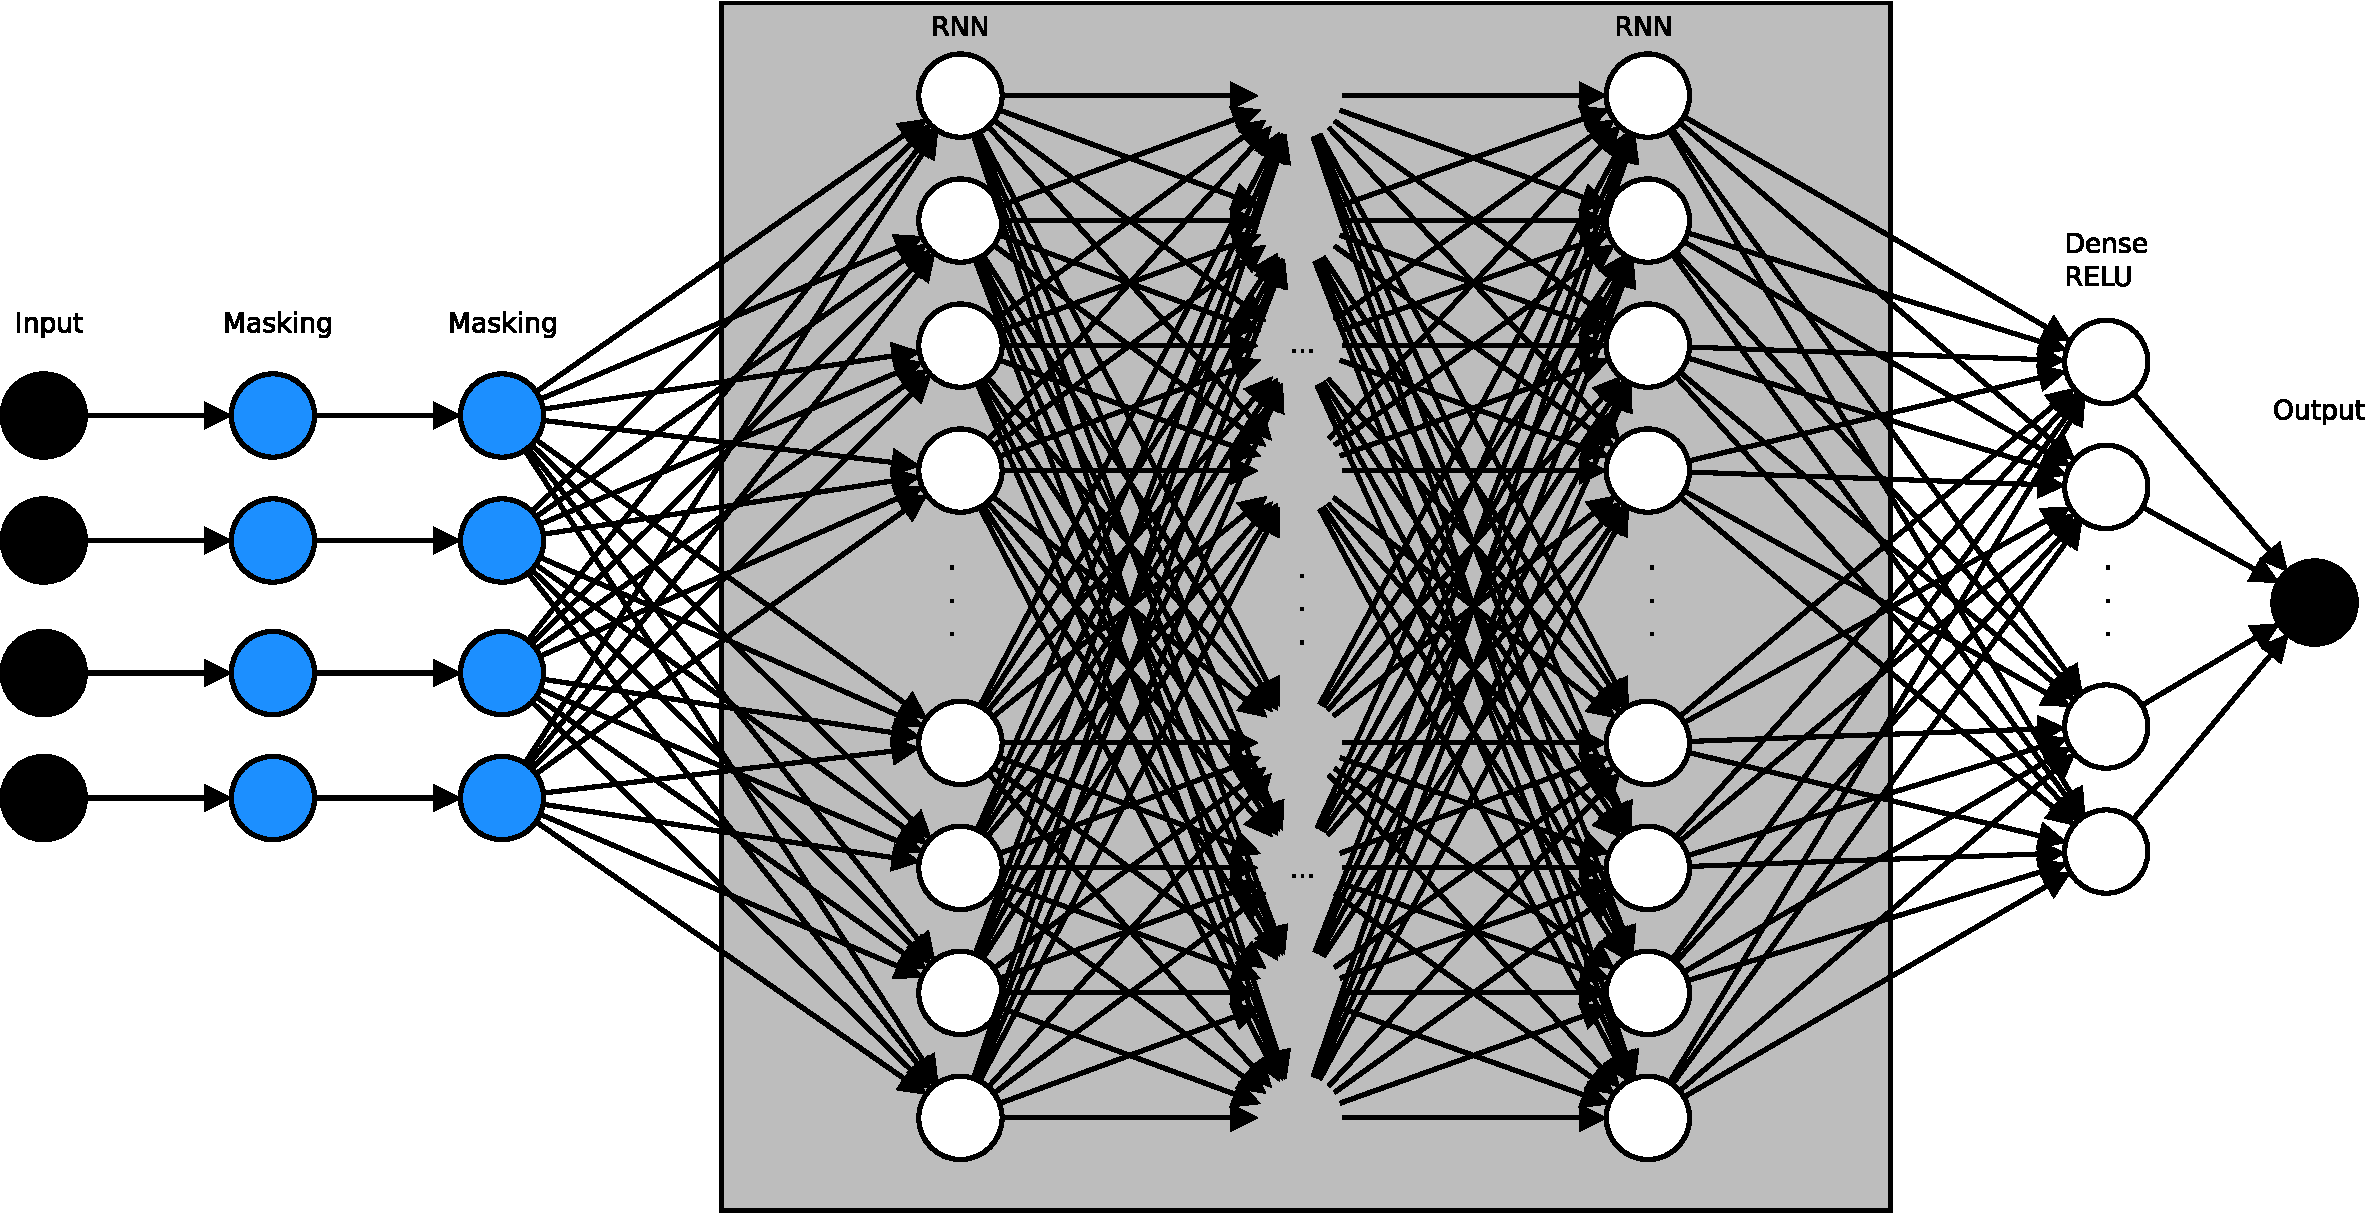
\includegraphics[width=\textwidth]{Model.pdf}
    \caption{Our NN Model has two masking units per input, a number X of RNN units on Y layers, pedenting on the experiment, as well as half as much units of Dense RELUs and one Dense unit with the sigmoid activation on the output layer.}
    \label{fig:Model}
\end{figure}

% % TODO: talk about flow+packet concat as another "sanity check" experiment?
% As described in the Input section above, we will try to avoid a concatenation of each packet with the flow data.
% However it might be interesting to see if it even has an impact on the performance.

% % TODO: masking with one or two layers?
% As described in the dataset preparation section of this work, our NN will need two masking layers.
% One for the UDP padding and one for the padding of the packet sequence length.
% To decrease calculation overhead, we propose to use only one masking layer and only one masking value instead of two.
% This idea might be flawed so experiments comparing both approaches are in order.

% % TODO: another experiment would be to not convert the categorical data, but instead just use a int/bool mix vector and see where it goes
% %       also easy todo as this is what we did so far anyway
% Also skipping the conversion of categorical data into a continuous vector could yield interesting results.

% FIXME: depending on the size of the training split into separate sections, like before

\chapter{Experiments}
\label{sec:experiments}

In this chapter, we discuss the experiments conducted on the dataset(s) and the NN models described in the previous chapters.
We initially planned to compare the different RNN architectures, simpleRNN, LSTM and GRU.
However as our model performed suboptimally, we first shifted our focus to debugging of the model, solving our problem with one of the architectures and finding the hyperparameters, for which our model achieved the best performance.
Even though we still aimed to compare the three RNNs, we first needed to figure out, how one of the RNNs could be trained effectively.
For this reason, most of our experiments are only done with an \textbf{LSTM}-based condRNN model, or conditional LSTM (condLSTM) model.
We later compare the model to simpleRNNs and GRUs.

\section{Dataset statistics}
\label{sec:datasetStats}

We created multiple datasets from our source packet captures.
For testing on our local machine, we first creased a \textbf{base} dataset that was constructed from 5\% of our available data.
After achieving poor performance we created four additional datasets.
For the experiments on the compute server, we created a \textbf{full} dataset from the complete set of data we sampled from our source packet captures.
The \textbf{full} dataset has 378410 total datapoints, including 227499 positive datapoints and 150911 negative datapoints.
To keep the compute time reasonable we used only 10\% (\textbf{full10}) and 25\% (\textbf{full25}) of the complete dataset at random.

The other three of which were based on the same data, but as the first had only minimal errors in the negative samples, we now created datasets with more errors.
First, we increased our from 1 error per packet to \textbf{9 errors} per altered packet.
Then, we increased the negative samples by a factor of three. This dataset we call \textbf{more negatives}.
Alternatively, we created a dataset that altered not just one but up to \textbf{20 packets}.
See table \ref{tab:negativeSamples} for the detailed breakdown of parameters used to create these datasets.
Each dataset had an equal share of each method of negative sample generation described in section \ref{sec:negativeSamples}.
The difference between the datasets is the degree of errors per negative sample and the number of negative samples added.

The datasets \textbf{base}, \textbf{9 errors}, and \textbf{20 packets} did not differ too much in regards to the number of datapoints and therefore in the ratio of positive to negative datapoints, as can be seen in table \ref{tab:datapoints}.
The datasets \textbf{9 errors}, \textbf{more negatives}, and \textbf{20 packets} have 9 errors per packet, but only \textbf{20 packets} has more than one packet altered per negative datapoint.
And the \textbf{more negatives} dataset is the only of the smaller datasets with significantly more datapoints, as more negative samples are generated to provide a greater sample pool per negative sample creation method.

% where to put this
We also created a pure dataset for each method of negative sample creation (\ref{sec:negativeSamples}).
They all use the parameter configuration the base dataset used, which is applicable to their method.
And except for \textbf{method 3}, which had only 16890 datapoints with 6606 negative datapoints, they all had 20568 datapoints total and an even split of positive and negative datapoints.
We used these datasets to compare the different methods to create negative samples for out dataset.
We named the datasets method X, where X is the number of the method used to create it.
Note that \textbf{method 1a} refers to the creation of false packets by random data and \textbf{method 1b} refers to the creation of false packets by extraction from within the dataset, read more in section \ref{sec:negativeSamples}.

% all datasets share
% num_pkts=1, num_errors_flow=0, num_errors_from_dataset=None, num_errors_flow_from_dataset=None

% dataset (local), test2_dataset (hulk)
% num_errors=3, reduce_percentages=[0.1, 0.25, 0.5], num_packets=0

% dataset_clean_flows (hulk)
% num_errors=3, reduce_percentages=[0.1, 0.25, 0.5], num_packets=0
% total datapoints:  378410
% positive datapoints:  227499
% negative datapoints:  150911
% datapoints used total:  94602
% datapoints used for training:    66221 (70%)
% datapoints used for validation:  9460 (10%)
% datapoints used for testing:     18920 (20%)

% dataset_harder
% num_errors=9, reduce_percentages=[0.5, 0.75, 0.9], num_packets=50

% dataset_harder_more_negatives
% num_methods=2, num_errors=9, reduce_percentages=[0.5, 0.75, 0.9], num_packets=50

% dataset_hard
% num_pkts=20, num_errors=9, reduce_percentages=[0.5, 0.75, 0.9], num_packets=50

\begin{table}
    \centering
    \begin{tabular}{|c|c|c|c|c|c|}
        \hline
        % FIXME: column names
        % per packet, number of false, percentages, packets
        \textbf{name} & \shortstack{\textbf{errors} per\\ packet} & \shortstack{false\\ \textbf{packets}} & \shortstack{\textbf{reduce}\\ percentages} & \shortstack{\textbf{add}\\ packets} & \shortstack{sample\\ \textbf{factor}} \\
        \hline
        base & 3 (1-8) & 1 & 10\%, 25\%, 50\% & 0 (1-10) & 1 \\
        \hline
        9 errors & 9 (4-14) & 1 & 50\%, 75\%, 90\% & 50 (40-60) & 1 \\
        \hline
        more negatives & 9 (4-14) & 1 & 50\%, 75\%, 90\% & 50 (40-60) & 3 \\
        \hline
        20 packets & 9 (4-14) & 20 (15-25) & 50\%, 75\%, 90\% & 50 (40-60) & 1 \\
        \hline
        full & 3 (1-8) & 1 & 10\%, 25\%, 50\% & 0 (1-10) & 1 \\
        \hline
    \end{tabular}
    \caption{Negative sample statistics from datasets.}
    \label{tab:negativeSamples}
\end{table}

\begin{table}
    \centering
    \begin{tabular}{|c|c|c|c|c|c|}
        \hline
        \shortstack{dataset\\ \textbf{name}} & \shortstack{\textbf{total}\\ datapoints} & \shortstack{\textbf{positive}\\ datapoints} & \shortstack{\textbf{negative}\\ datapoints} & \shortstack{\textbf{percentage}\\ \textbf{used}} & \shortstack{datapoints\\ \textbf{total used}} \\
        \hline
        base & 18977 & 10284 & 8693 & 100\% & 18977 \\
        \hline
        9 errors & 18086 & 10284 & 7802 & 100\% & 18086 \\
        \hline
        more negatives & 29550 & 10284 & 19266 & 100\% & 29550 \\
        \hline
        20 packets & 16693 & 10284 & 6409 & 100\% & 16693 \\
        \hline
        full10 & 378410 & 227499 & 150911 & 10\% & 37841 \\
        \hline
        full25 & 378410 & 227499 & 150911 & 25\% & 94602 \\
        \hline
    \end{tabular}
    \caption{Datapoints per dataset.}
    \label{tab:datapoints}
\end{table}

\section{Experimental Setup}
\label{sec:exSetup}
\label{sec:exTrainTest}

% TODO: mention that we used LSTM for most of this reasoning

For the initial training of our model we used only around 5\% (base) and 10\% (full10) of the data available to us as not to exceed the resources, specifically memory, of the systems we used and reduce compute times.
A workstation with an AMD Ryzen 5 3600 6-Core @ 12x 3.6GHz and 32GB of ECC memory and a compute server with the Tesla V100S GPU also with 32GB memory.
As our experiments progressed and we required more memory, we had to switch to CPU processing on the compute server.
Giving us a share of the 48 threads @ 3.0GHz and 504GB of ECC memory.
Even though we had longer compute times, this at least allowed us to run experiments with 25\% of our dataset (full25) and use more than 96 units within an RNN layer.
% FIXME: edit on final experiments
We later hoped to increase this even further to 50\%, but the computation time would not allow it, as too much time was already spend on debugging and optimizing the model.

For training we used
%Training the NN appeared as a problematic task, as
The model did not seem to achieve more than 60\% accuracy.
The accuracy was most often pending around 57\% over multiple experiments.
As our \textbf{base} dataset (section \ref{tab:datapoints}) had the same ratio of positive to negative datapoints, we assumed the true accuracy of our model to be 50\% at best, so not better as a coin toss.

Our model for the experiments consisted of two masking layers, which provided the RNN layer with the mask for UDP and packet padding,
up to four condRNN (LSTM) layers with up to 128 units,
a dense layer with ReLU activation and half as many units as an RNN layer,
and a dense layer with a sigmoid activation unit for the output.
This was manually implemented as a \code{keras.Model}, since the condRNN layer, which accepts two inputs, is incompatible with \code{keras.Sequential} at this point in time, as it only supports a single input.
For the condRNN layer we used the \code{cond-rnn} library \cite{remyPhilipperemyCondRnn2020}.

% LOSS FUNCTION
In our earlier experiments we used \textbf{sparse categorical cross-entropy} as a loss function, but this function was ill-suited for our problem.
Once we figured this out we switched to the \textbf{binary cross-entropy} loss function, which is best suited for binary classification problems.
Combined with a \textbf{sigmoid activation} for our output layer this helped us obtain better results.
We also compared our results to the \textbf{hinge} loss function in combination with the \textbf{hyperbolic tangent} (tanh) function on the output hoping for a steeper learning curve, as it provides a greater punishment for misclassification with the wrong signage.
We thought this might be beneficial to our cause, but as it turns out it only led to worse results, see figure \ref{fig:hinge}.

Throughout our experiments, we always used 70\%, 10\%, and 20\% of the used dataset for training, validation, and testing respectively, as it is the most common segmentation of data.
We started with 5 to 20 epochs for initial testing of hyperparameter combinations and went up to 100.
Once a combination of hyperparameters looked promising, we went up to as far as 1000 epochs.
In each epoch, the whole training dataset is used and processed in batches of size 100 to 1000.
Afterward, the model gets validated by the validation dataset.
During training the weights get updated after each batch. % and at the end of an epoch after the validation.
After all training and validation epochs are finished the model was evaluated on our test dataset.
We soon came to realize that there is not much change to be seen after 100 epochs.

\section{Evaluation of Results}
\label{sec:exEval}

% disclaimer
When we talk about accuracy or loss in this section we generally talk about validation accuracy and validation loss, unless stated otherwise.
As they were very similar to the training accuracy and loss, in most experiments slightly better and give a clearer understanding about the model's performance than test accuracy and test loss.
Since the validation is repeated for each epoch and the testing is only done once after the model was trained, the validation can provide a look at the performance of the model over time.

% EPOCHS
Usually, the validation accuracy increases over the first three to 20 epochs, depending on the experiment and its hyperparameters, then just hovers close to its average value, e.g. 57\%, and flattens slightly above it.
Sometimes it increased more slowly, but even 1000 epochs weren't enough to reach a decent accuracy and resulted in the same behavior, see figure \ref{fig:1000epochs}.
The validation loss behaves similarly it decreases fast than slower and eventually flattens close to its average.
% TODO: sample graph

% LAYERS
However we still only reached an accuracy of 59\% at best with one RNN layer of up to 64 units.
During our earlier experiments, we concluded 3 or 4 layers to produce the best results again going any higher than 4 usually did not improve the accuracy and only produced additional overhead in computing time.
With 3 layers and 64 per layer, we were able to produce an accuracy of 60\% to 63\% within the first 15 epochs, while the loss was consistently decreasing.
Since the switch to binary cross-entropy however, we saw the same behavior, only this time 1 or 2 layers seem to achieve better results than 3 or 4 layers, see figure \ref{fig:layers}.

% UNITS
We tried RNN layers with 32, 64, 96, 128, 192 or 256 units.
However, we found anything above 128 did not provide better results in relation to the compute time.
We believe the optimal number of units to be between 64 and 128.
If we compare their performance in figures \ref{fig:units} and \ref{fig:units25}, we see that 96 units provide the best results on average and over-all.
This goes for our model with both one and two layers as well as our base and full25 datasets.

% BATCHSIZE
For the batch size of 300 to 350 to be most effective to achieve a good decrease of loss.
As we can see in figure \ref{fig:batchsize} the batchsize of 1000 provides the worst results by far.
While 500 provides better results, it was not able to crack 63\% accuracy.
Everything under 500 shows more promising results, especially 350, which as an average validation accuracy of 63\%.
But going lower than that we see slightly worse results again, as we can see with 300 in the graph.
%The described behavior and its improvements can be seen over all parameters.

% Datasets
For the dataset(s) we mainly considered two types of comparison.
One the percentage of the complete dataset or the number of datapoints.
Two the number of errors for negative datapoints.
% datapoints
For the first type, we used our smaller dataset with 18977 datapoints, which is roughly 5\% of our total data, and compared it to 25\% of our total dataset, which amounts to 94602 datapoints.
We saw an improvement of both accuracy and loss here, however not regarding the general behavior of the model, but rather a shift of the curve along the y-axis, see \ref{fig:dataset_percentage}.
However, it is to be noted that for the larger dataset (full25) the number of layers and units seems to make a bigger difference in performance compared to the dataset with less datapoints.
Increasing the units from 32 to 64 increases the average accuracy by 3.5\% with the full25 dataset, while the base dataset only shows an increase of around 1\%.
% random spike in 64u 1l -> due to the randomly selected samples
% number of errors
For the second type, we used the datasets with different configurations of negative samples described in section \ref{sec:datasetStats}.
As we can see in figure \ref{fig:dataset_negative} the more negative samples in a dataset (3 times) does improve the average accuracy (and loss).
However, it does cause more fluctuation in the accuracy over time and the flattening worsens.
We conclude that the improvement is merely based on the additional data available not on the increase of negative samples.
Adding more altered packets to our first method of negative sample creation, marked in the graph with `20 packets', did improve accuracy and loss.
Even though it gave a significant shift along the y-axis it did not change the behavior of the model overall.
% It might be interesting though to give it another look for future work, as it seemed to be one of the view experiments that showed near linear increase. This can also be a coincident of cause.
Increasing the number of errors per altered packet from 3 to 9 did increase the models accuracy a bit, but again only by shifting the curce along the y-axis.

Regarding different error types, we also performed an experiment with datasets with negative datapoints created by only one of the method described in section \ref{sec:negativeSamples}.
The results can be seen in figure \ref{fig:negative_methods}.
As we can see, \textbf{method 1a} and \textbf{method 2} caused the most problems for our model.
This is of no surprise, as \textbf{method 1a} generates random numerical values within the scope of the header fields, meaning their size in bit, so the model might only see those numbers in those negative samples and \textbf{mothode 2} randomizes the order of packets and not their contents, which is hard to detect in comparison to a flow, especially for UDP.
For UDP it might in fact be impossible.
% FIXME FOR DISCUSSION: It has been an error to assume just randomizing any packet order yields good negative samples. It is good to have such difficult samples, but not all of them are necessarily false. ... TODO: more
\textbf{Method 1b} on the other hand performs average in comparison with the general results of the model.
This again can be easlily explained, as the method takes a number of fields from other datapoints in the dataset at random and adds them to an otherwise positive sample.
The model has to struggle as it knows all values from other positive datapoints, but it also is able to pick up to which datapoints the values belong.
\textbf{Method 3} and \textbf{method 4} perform the best in our model with up to 75\% validation accuracy and an average validation accuracy of above 70\%.
This is interesting to note.
However they have samples they struggle with and drop the validation accuracy as low as 52.5\% (method 3) and 56\% (method 4), but mostly they stay above 65\%.
Their behavior is the most complex out of the methods.
The good performance of both is most likely due to the lack of unknown data, meaning data that is not present in the positive datapoints.
One could argue that \textbf{method 1b} should benefit from this as well, and it does, to a certain degree.
However, \textbf{method 1b} has viewer and more delicat changes. It alters header fields of a few packets, in most cases (as in this comparison) just one.
\textbf{Method 3} and \textbf{method 4} alter the sequence of packets, which is way more powerful, especially in regards to the recurrent architecture of our model.
As for the problematic samples, we assume that they had only small changes.
For example, they could have been created from positive samples with a small packet count and therefore only got a small reduction of packets (method 3), or two very similar flows got their packet sequence switched (method 4).
As we have a lot of short TCP flows, we deem this likely.

% TODO: introduce condLSTM and condGRU somewhere, or state that all NNs mentioned are conditional
% TODO: different RNNs
When we compare our LSTM-based model to the same model with simpleRNN layers, we see very similar accuracy and loss (figure \ref{fig:rnns}).
However, the difference lies in the detail here.
If we look at the graphs, we can see that simpleRNN has a lot more fluctuation than our LSTM.
This could be traced back to the vanishing gradient problem.
The simpleRNN can practically only hold a limited amount of previous results in his memory and therefore struggles with data the LSTM has no problems with.
% FIXME: present the old entropy comparison?
Unfortunately our model was not able to produce any results using GRUs since we switched to binary cross-entropy for the loss function.
The loss with GRUs was not computed correctly, therefore the accuracy did not change.
We instead ran the GRU with the hinge loss function, as we described earlier in this section, which at least was able to compute loss values.
However the accuracy did not even reach 25\%, see figure \ref{fig:GRUhinge}.

\subsection{Debugging}

% Initially our data was only around 3\% of the sampled data, but we achieved the same results with the complete dataset.
To debug our model we performed multiple sanity checks.
We tried a dataset using data from only one of the aforementioned NIDS dataset captures with no improvements.
Changing the architecture from the conditional RNNs to a normal RNNs did not change the overall behavior of the model too much, only created slightly worse accuracy, so a problem with the \code{cond-rnn} libraries implementation can be excluded for the most part.
This holds also for the manual model implementation, as a simple \code{keras.Sequential} implementation yields the same results.
We also tried running without the masking layers, anticipating worse results, as our masking values -10 and -15 were no longer excluded from the NN layer operations.
However, we saw no noticeable changes to accuracy.
Possibly our NN model was able to notice the marking values as not relevant data on its own, without the masking layers.
A higher number of ReLUs in the Dense layer also did not provide better results.
The model without the ReLU layer performed slightly better than with the ReLU layer,
at least regarding the validation accuracy and loss, but the flattened curves remained. % FIXME: wording
However, the validation loss decreased faster than the training loss and while the validation accuracy was better the training accuracy was worse.
So we returned to our original ReLU implementation.

\section{Discussion}
\label{sec:exDiscussion}

... This made us believe that the architecture of our model is inherently flawed.
Either that or our chosen features are not optimal yet.
The possibility that the data is not enough to obtain good results also remains.
Especially as we can only use up to 25\% of it.

It is no wonder that increasing the number of errors in negative samples increases the performance of the model.
%Same goes for increasing the amount of data.
However it can not be the solution to boost the model's performance by giving it easier samples to learn from.
In order to perform as a DN of a GAN proposed in the problem statement \ref{sec:problem} it would need to detect much smaller errors than we provided in our dataset(s).

The model has shown that with enough data and time, it might at least get to a higher accuracy.
But as it stands it is too inefficient to deliver good results in a reasonable amount of time.

\begin{figure}
    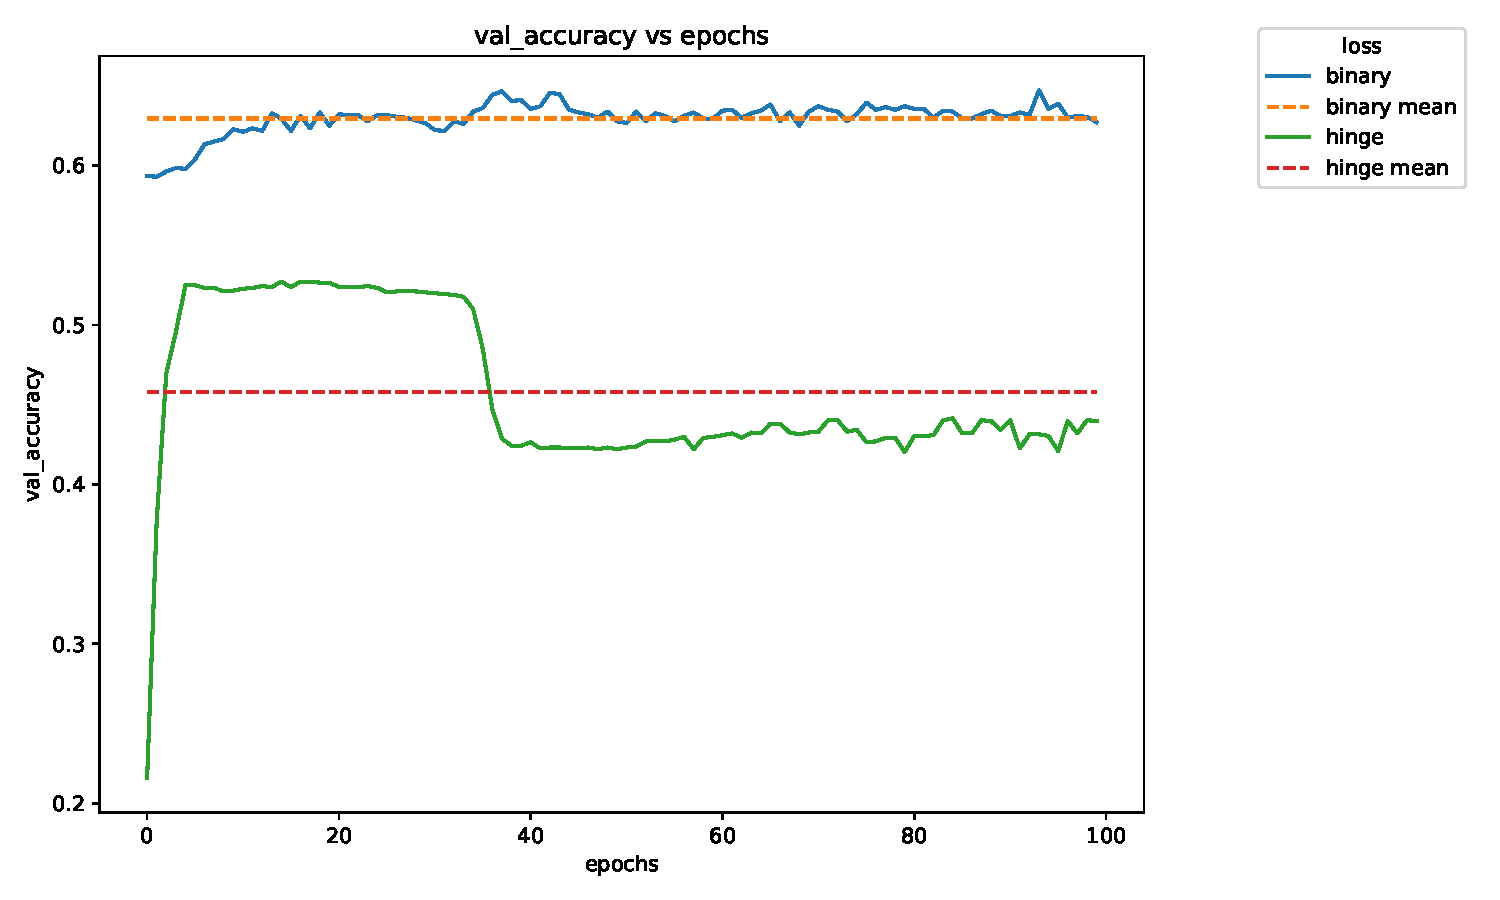
\includegraphics[width=.95\textwidth]{hinge_val_accuracy.pdf}
    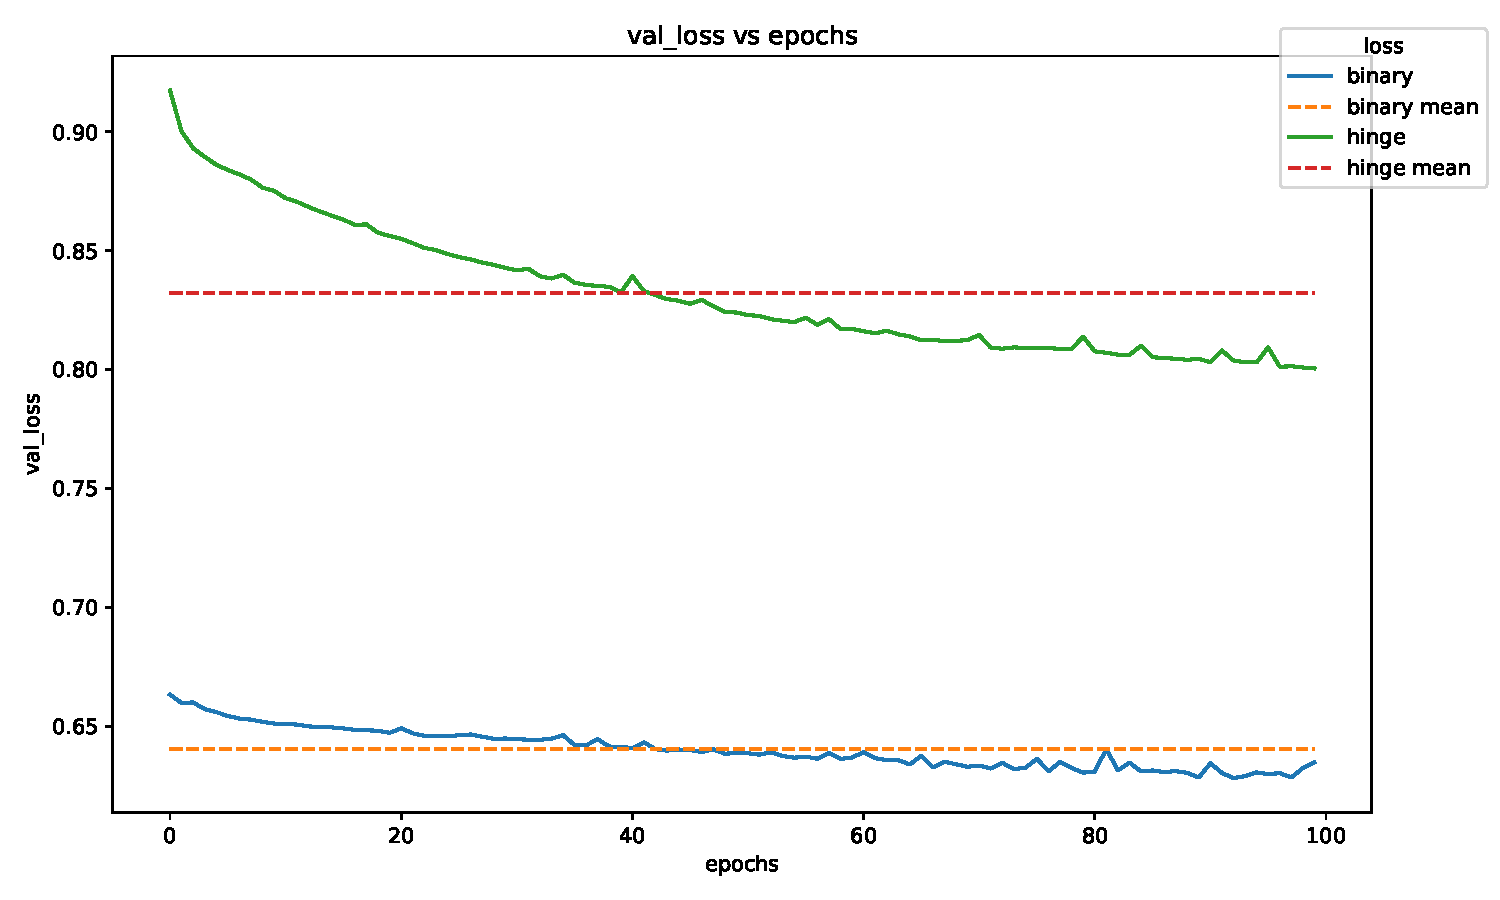
\includegraphics[width=.95\textwidth]{hinge_val_loss.pdf}
    \caption{Comparison of both validation accuracy and loss between \textbf{binary crossentropy} and \textbf{hinge loss}.
             Our model with 2 LSTM layers, and 64 units per layer was trained over 100 epochs with a batchsize of 350 and the \textbf{base} dataset.}
    \label{fig:hinge}
\end{figure}

\begin{figure}
    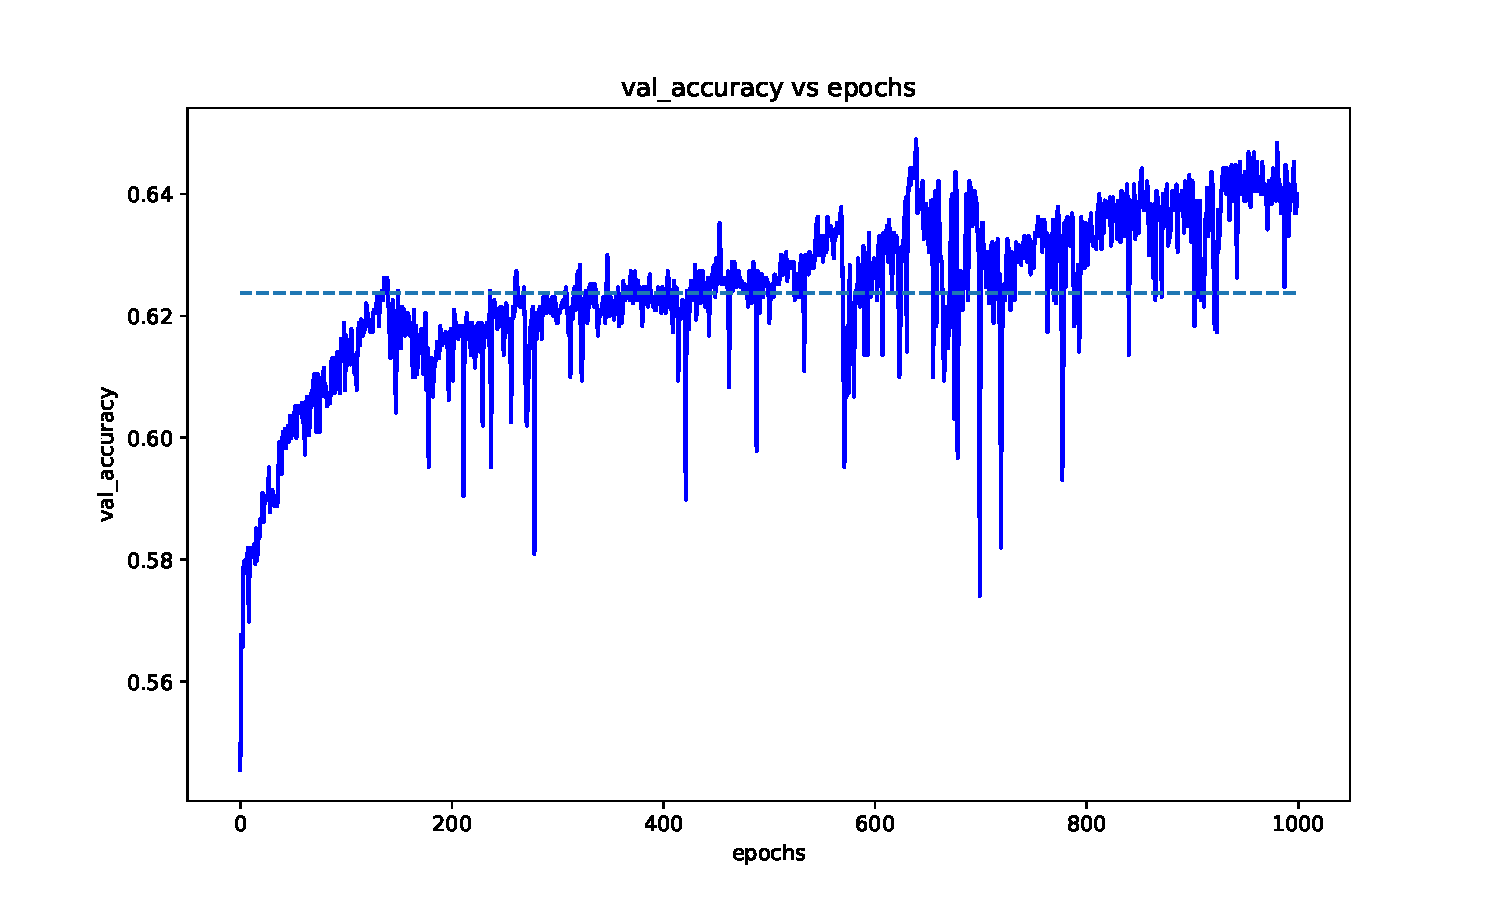
\includegraphics[width=.95\textwidth]{1000_val_accuracy.pdf}
    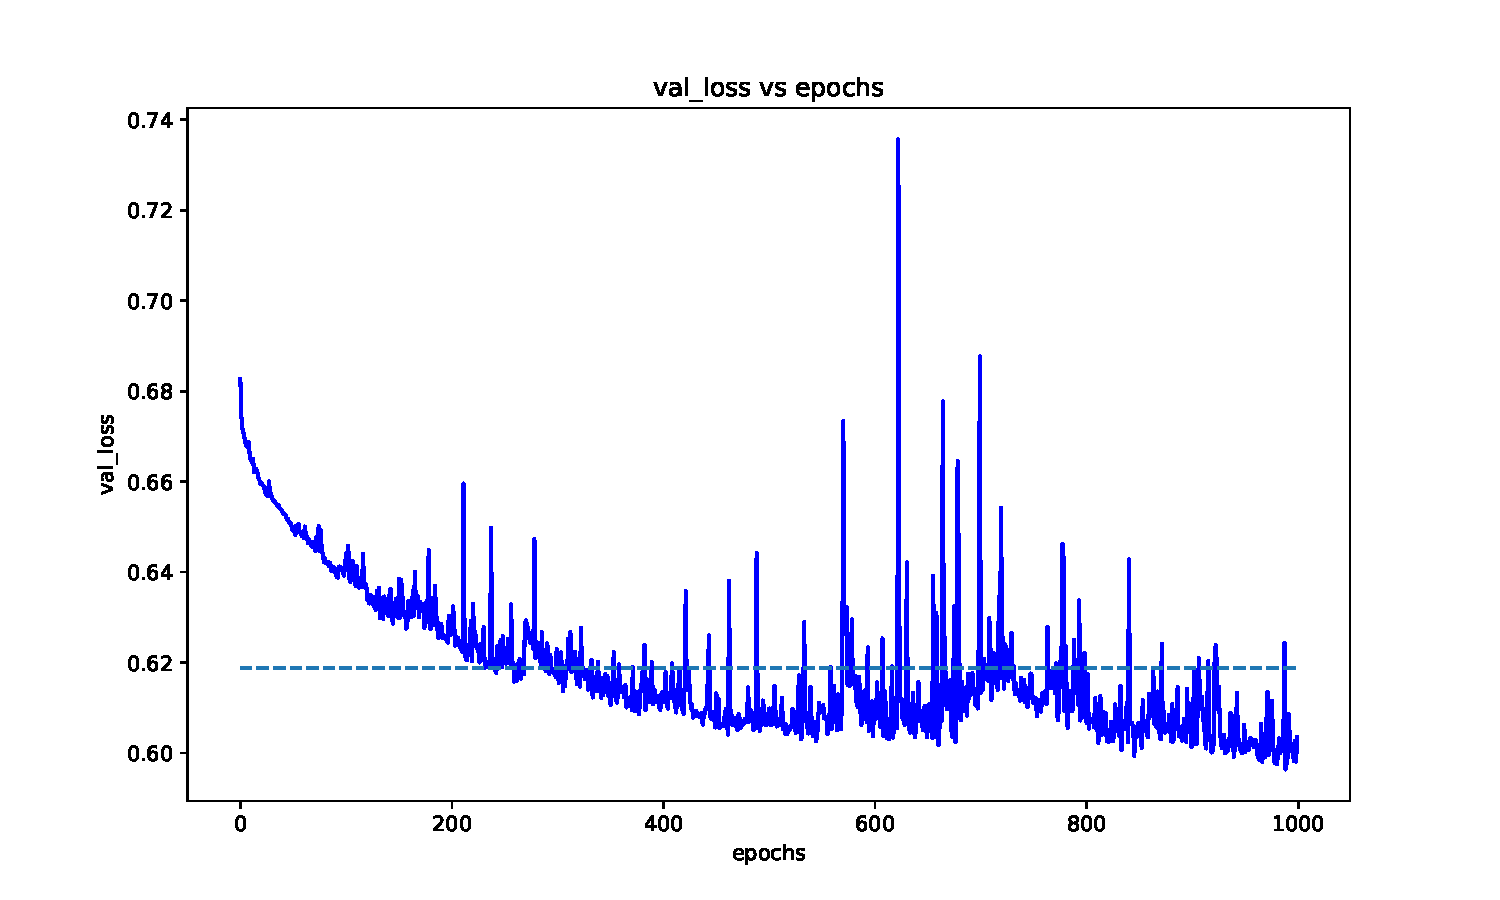
\includegraphics[width=.95\textwidth]{1000_val_loss.pdf}
    \caption{Validation accuracy and loss over 1000 epochs.
    Our model with 2 LSTM layers, and 64 units per layer was trained over 1000 epochs with a batchsize of 350 and the \textbf{base} dataset.}
    \label{fig:1000epochs}
\end{figure}

\begin{figure}
    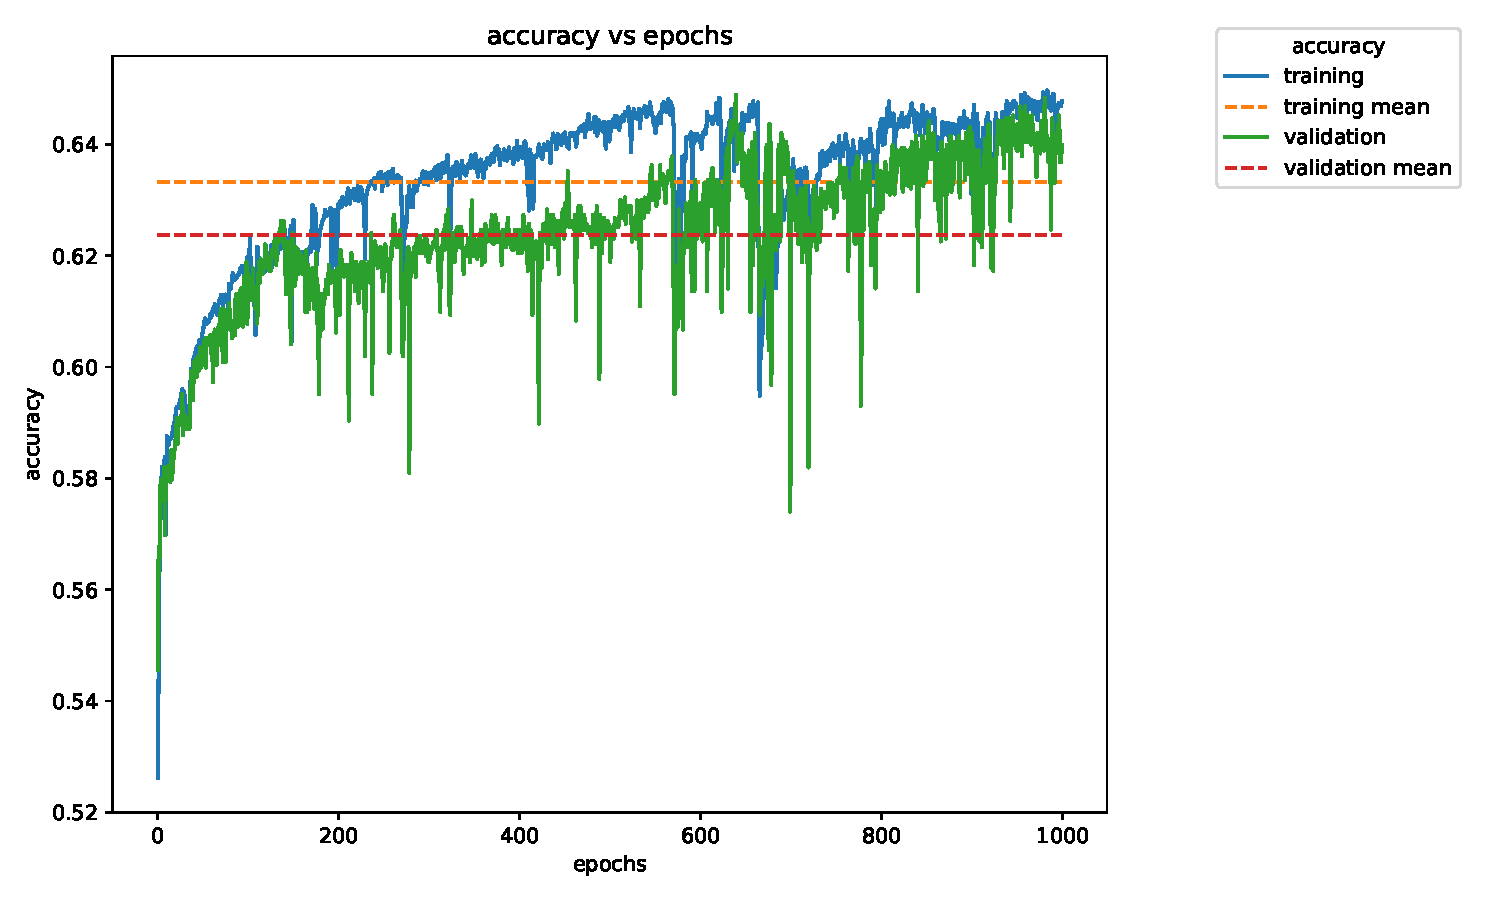
\includegraphics[width=.95\textwidth]{1000_comp_accuracy.pdf}
    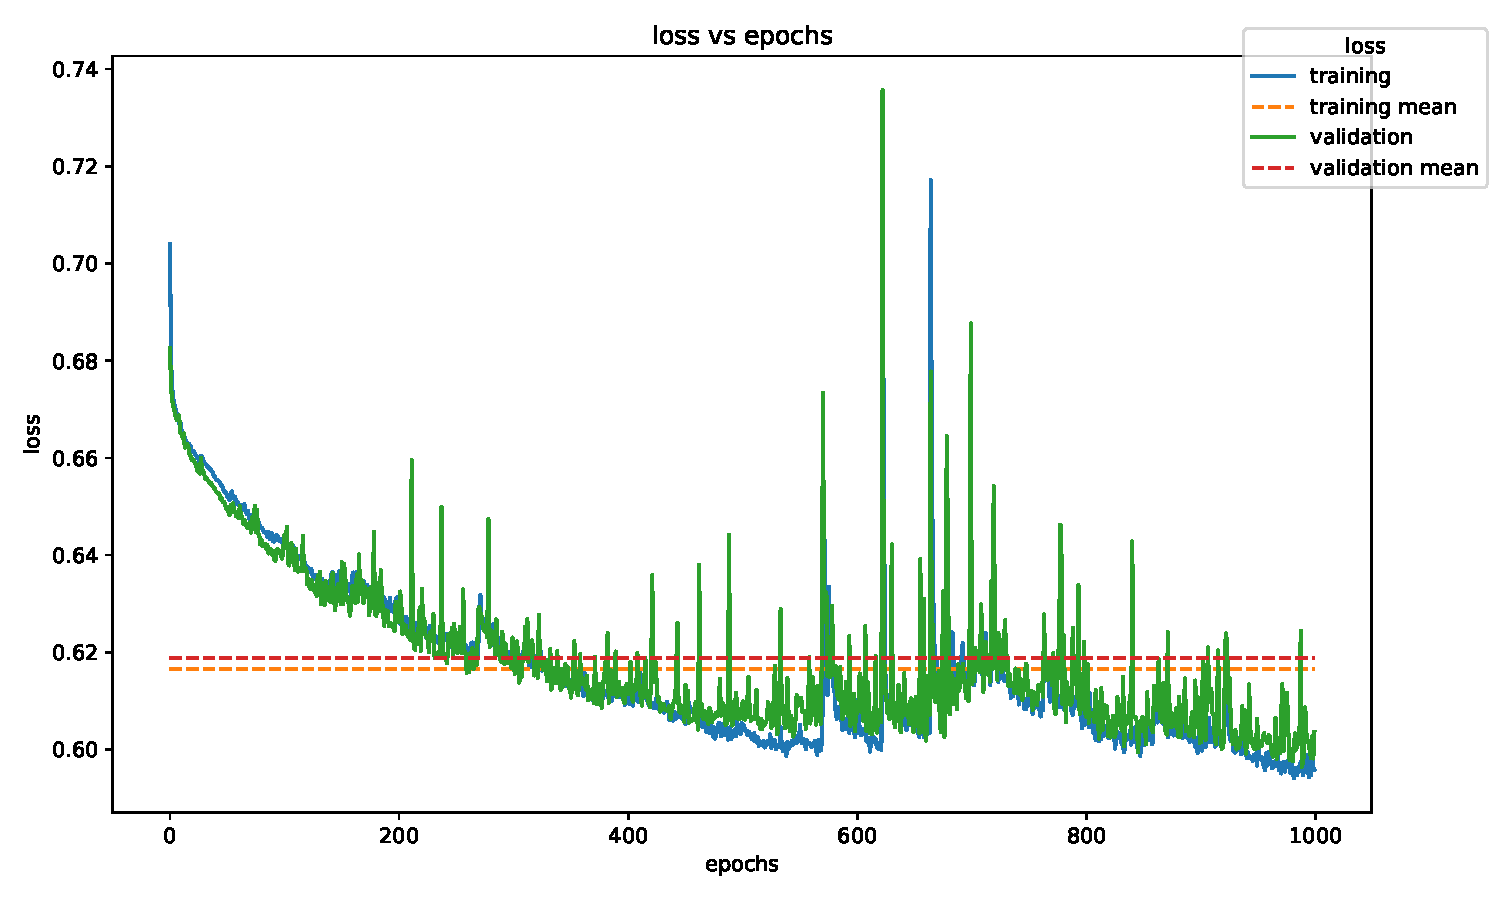
\includegraphics[width=.95\textwidth]{1000_comp_loss.pdf}
    \caption{comparison of accuracy and loss over 1000 epochs between training and validation.
    Our model with 2 LSTM layers, and 64 units per layer was trained over 1000 epochs with a batchsize of 350 and the \textbf{base} dataset.}
    \label{fig:1000comp}
\end{figure}

\begin{figure}
    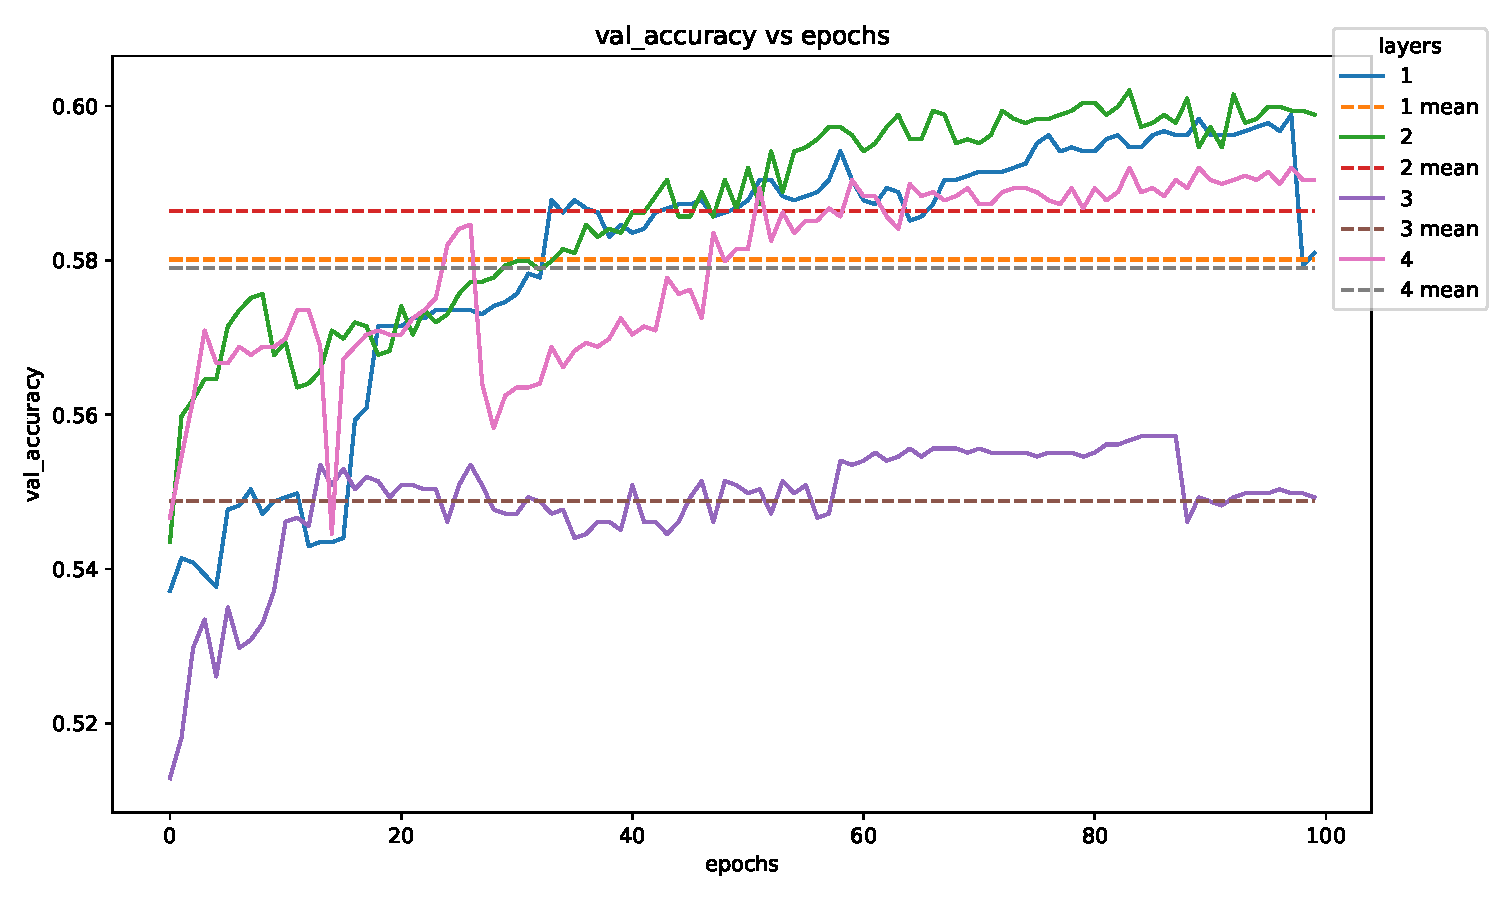
\includegraphics[width=.95\textwidth]{layers_val_accuracy.pdf}
    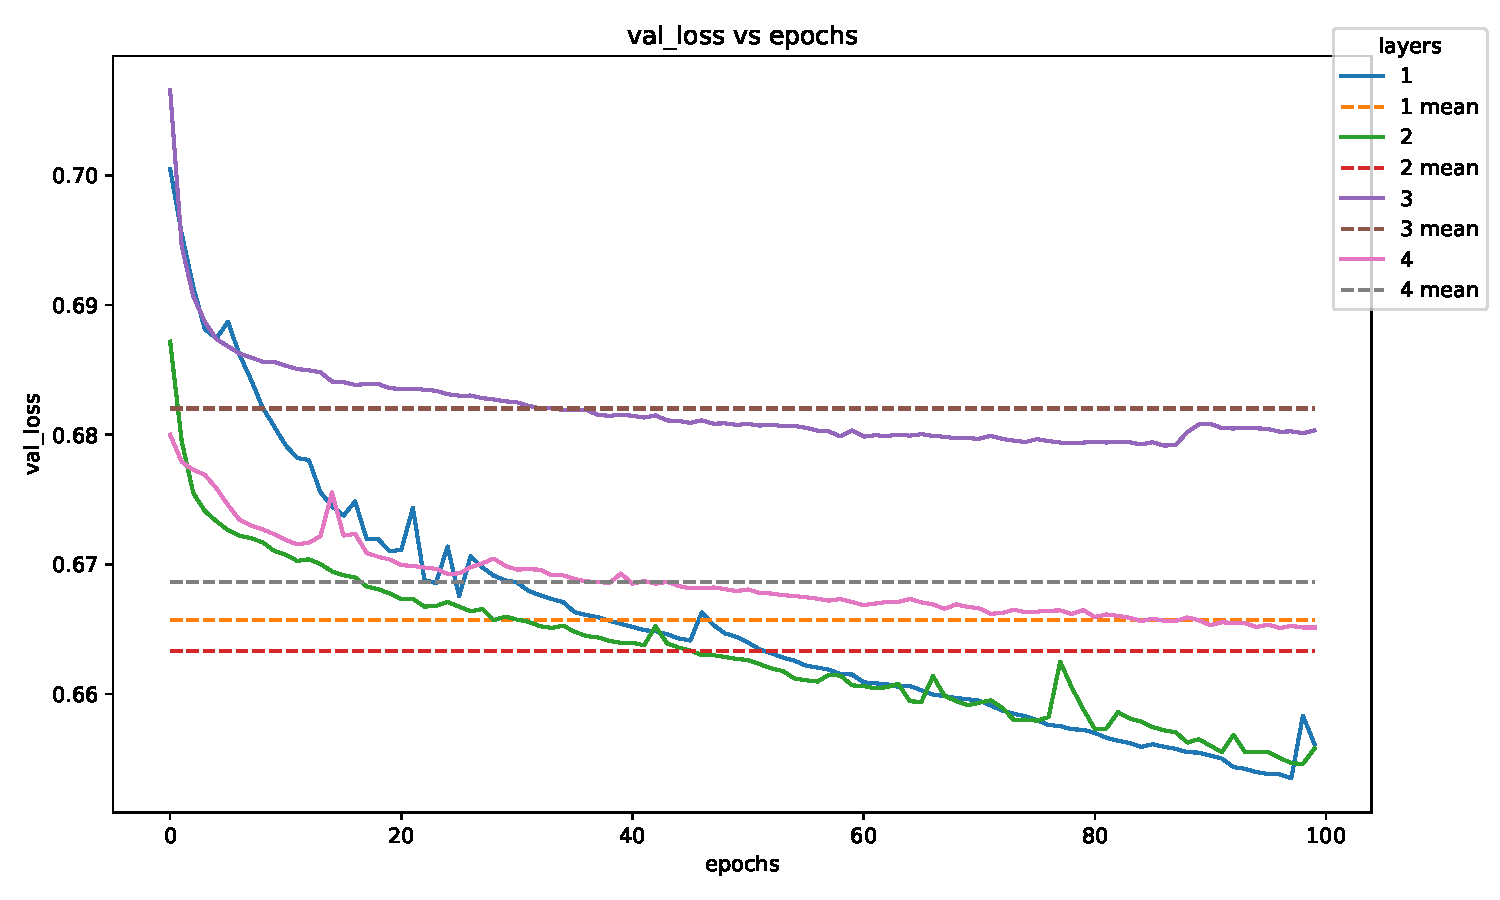
\includegraphics[width=.95\textwidth]{layers_val_loss.pdf}
    \caption{Comparison of both validation accuracy and loss between 1 to 4 layers.
    Our model with 64 LSTM units per layer was trained over 100 epochs with a batchsize of 500 and the \textbf{base} dataset.}
    \label{fig:layers}
\end{figure}

\begin{figure}
    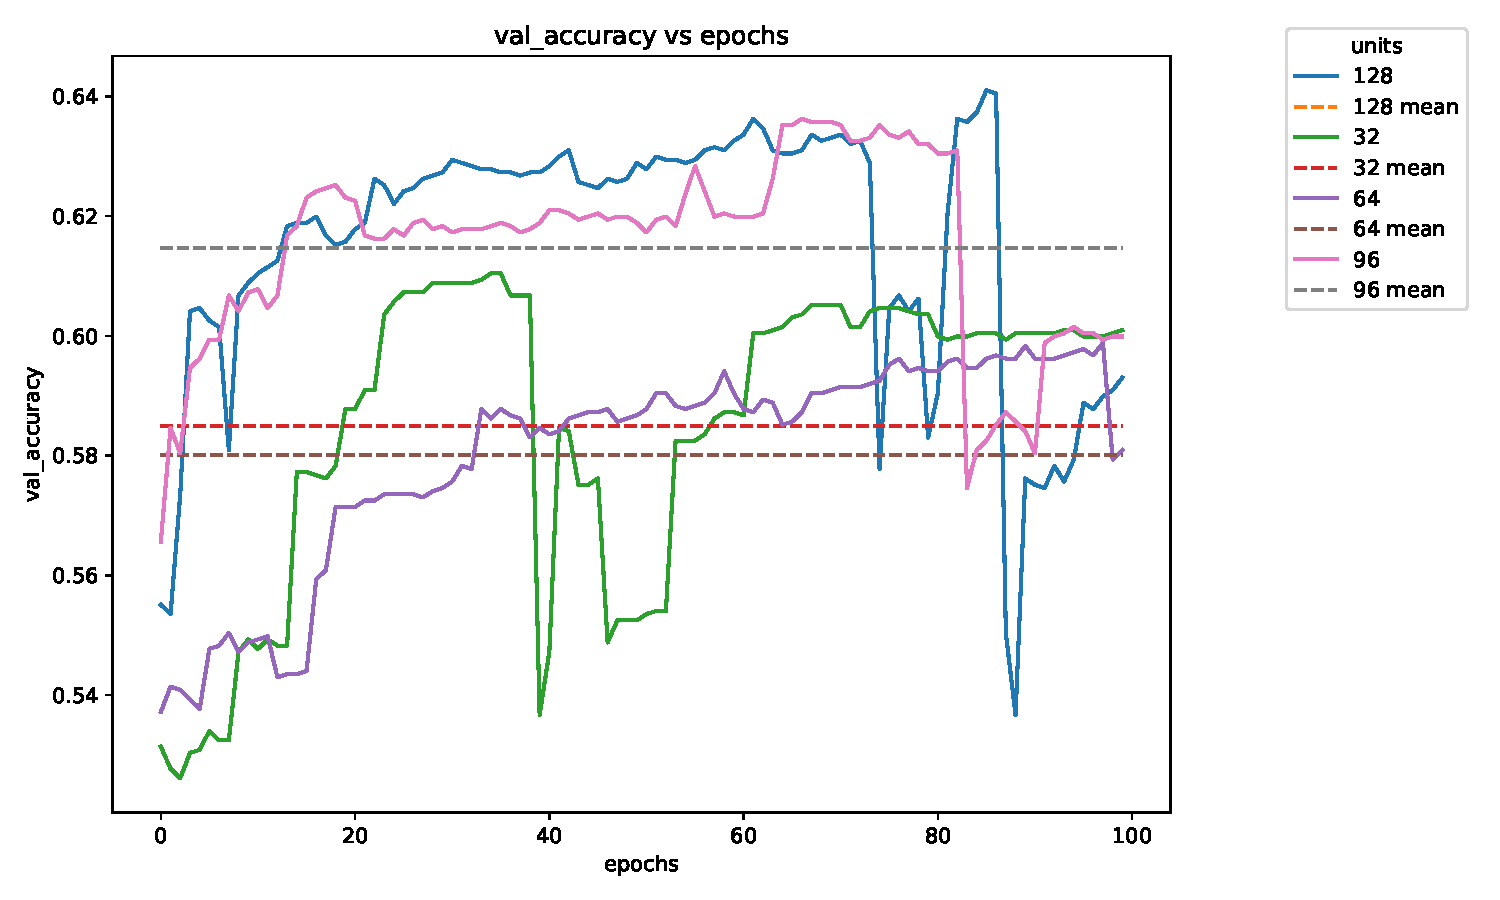
\includegraphics[width=.95\textwidth]{units_val_accuracy.pdf}
    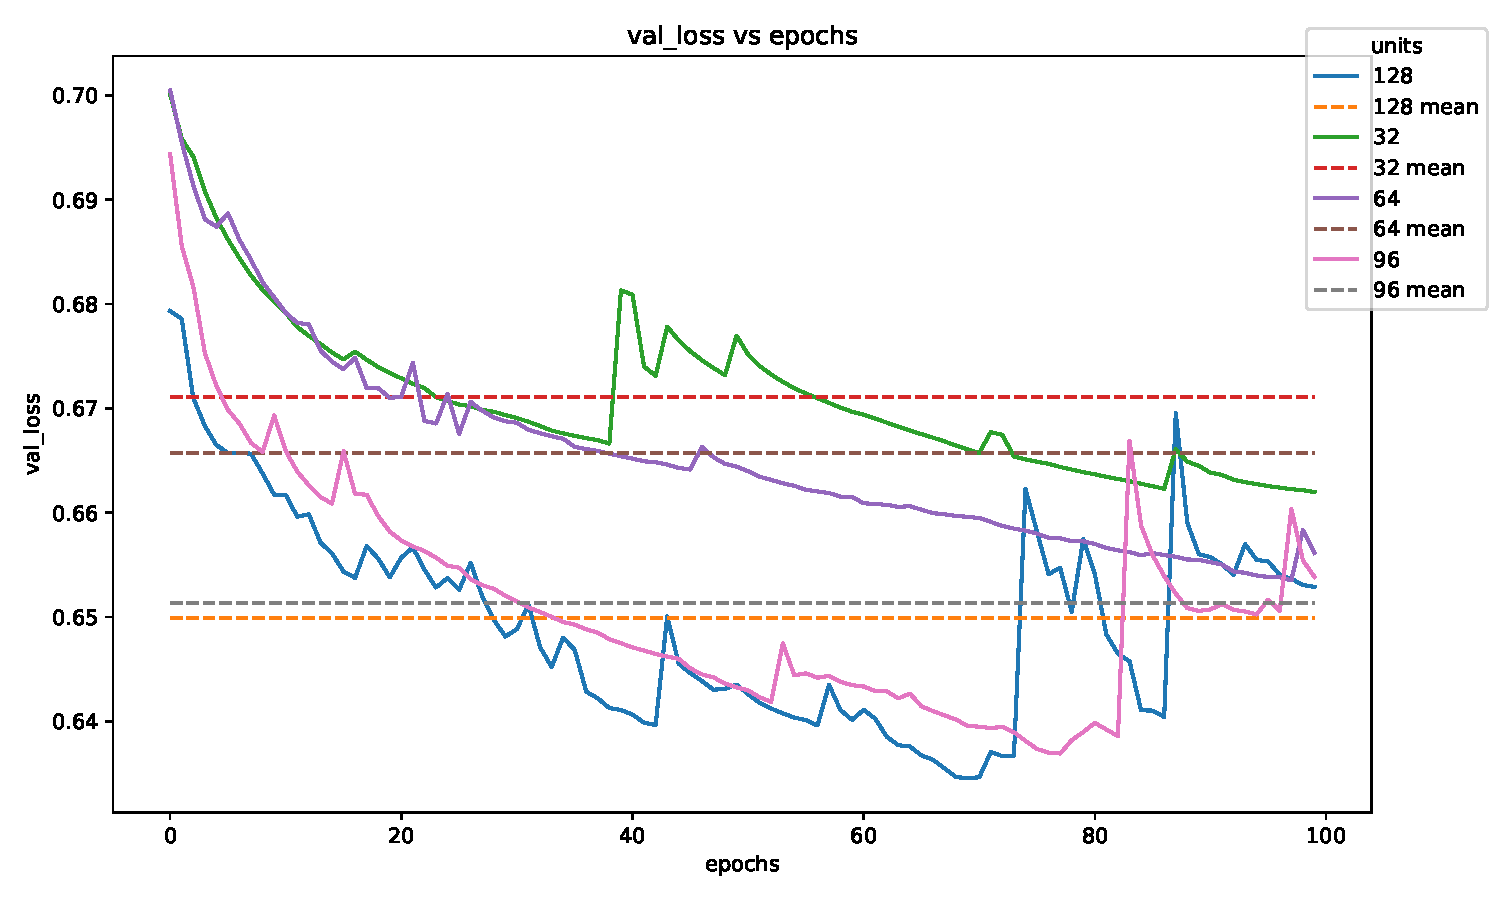
\includegraphics[width=.95\textwidth]{units_val_loss.pdf}
    \caption{Comparison of both validation accuracy and loss between x and y.}
    %TODO: parameters used dataset_dataset_LSTM_nn_1_layers_100_epochs_500_batchsize_18977_datapoint
    \label{fig:units}
\end{figure}

\begin{figure}
    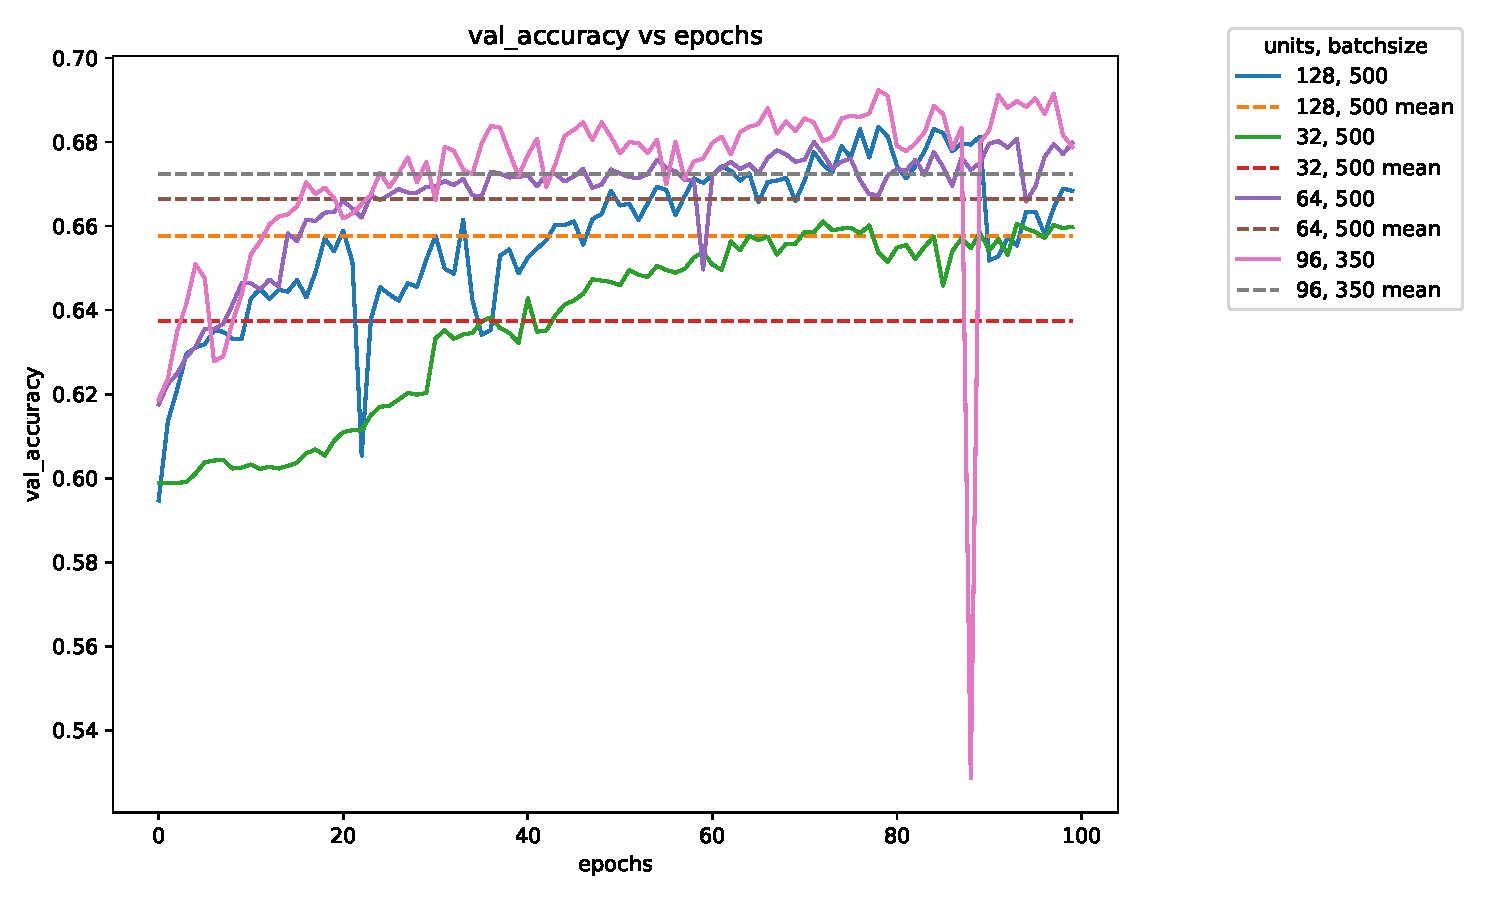
\includegraphics[width=.95\textwidth]{units25_val_accuracy.pdf}
    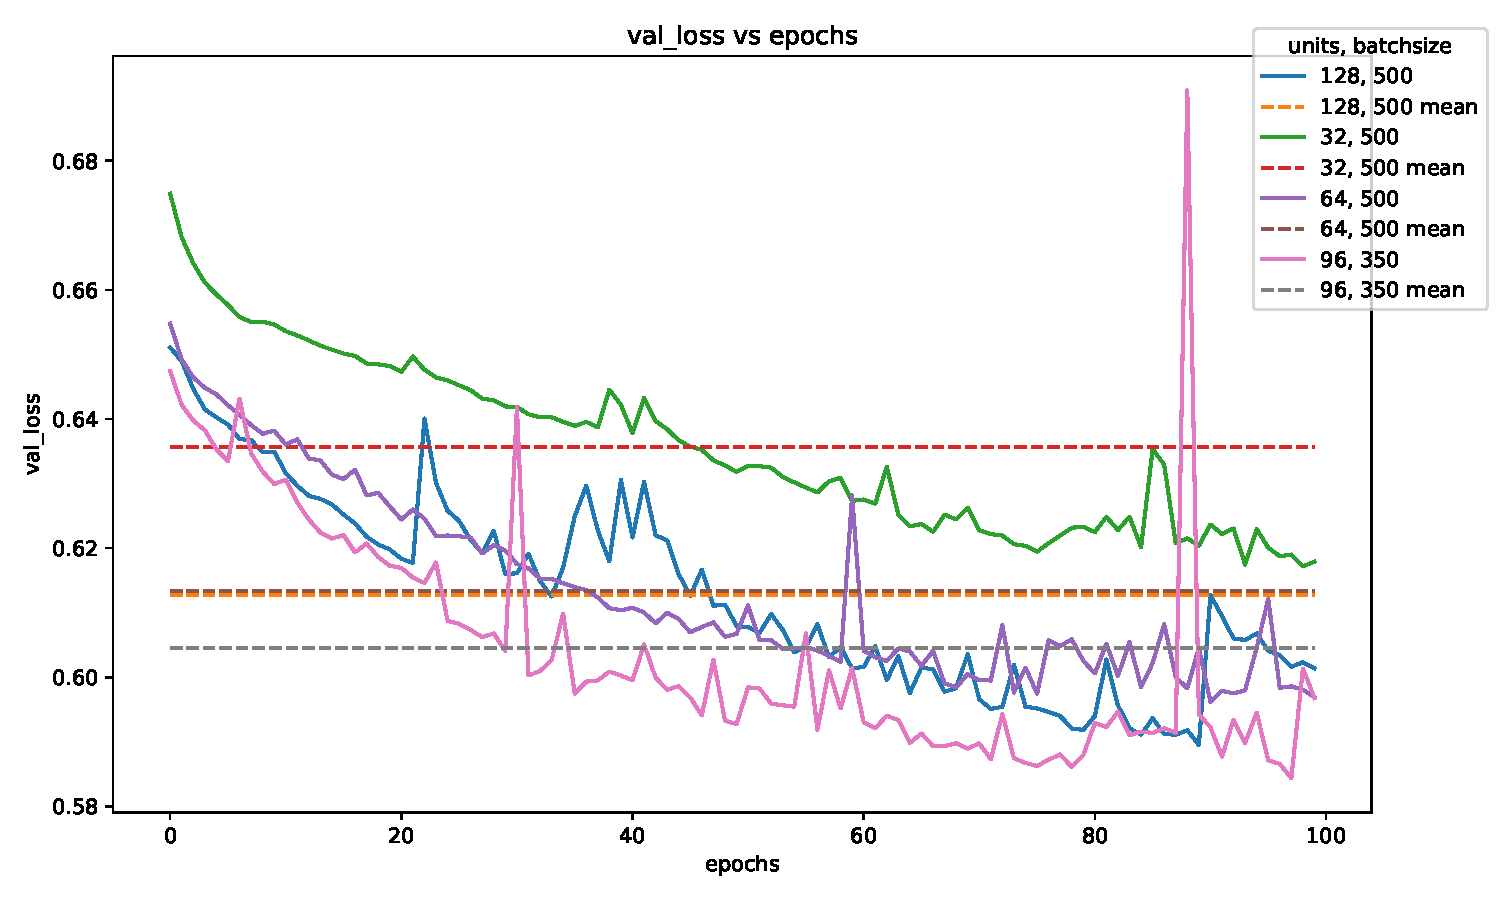
\includegraphics[width=.95\textwidth]{units25_val_loss.pdf}
    \caption{Comparison of both validation accuracy and loss between x and y.}
    %TODO: parameters used dataset_clean_flows_dataset_LSTM_nn_2_layers_100_epochs_94602_datapoint
    \label{fig:units25}
\end{figure}

\begin{figure}
    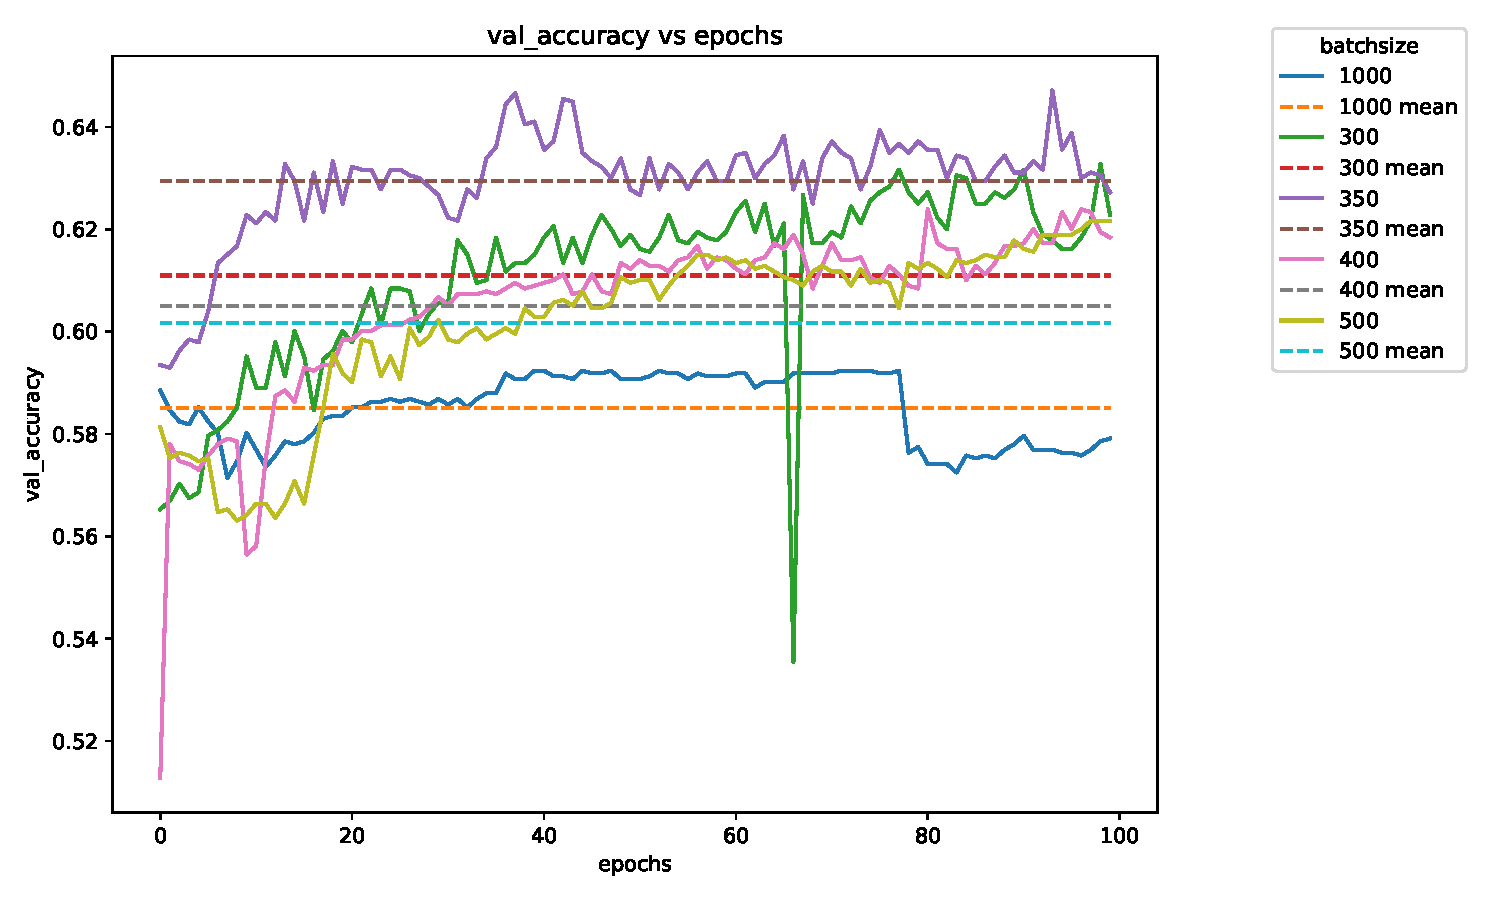
\includegraphics[width=.95\textwidth]{batchsize_val_accuracy.pdf}
    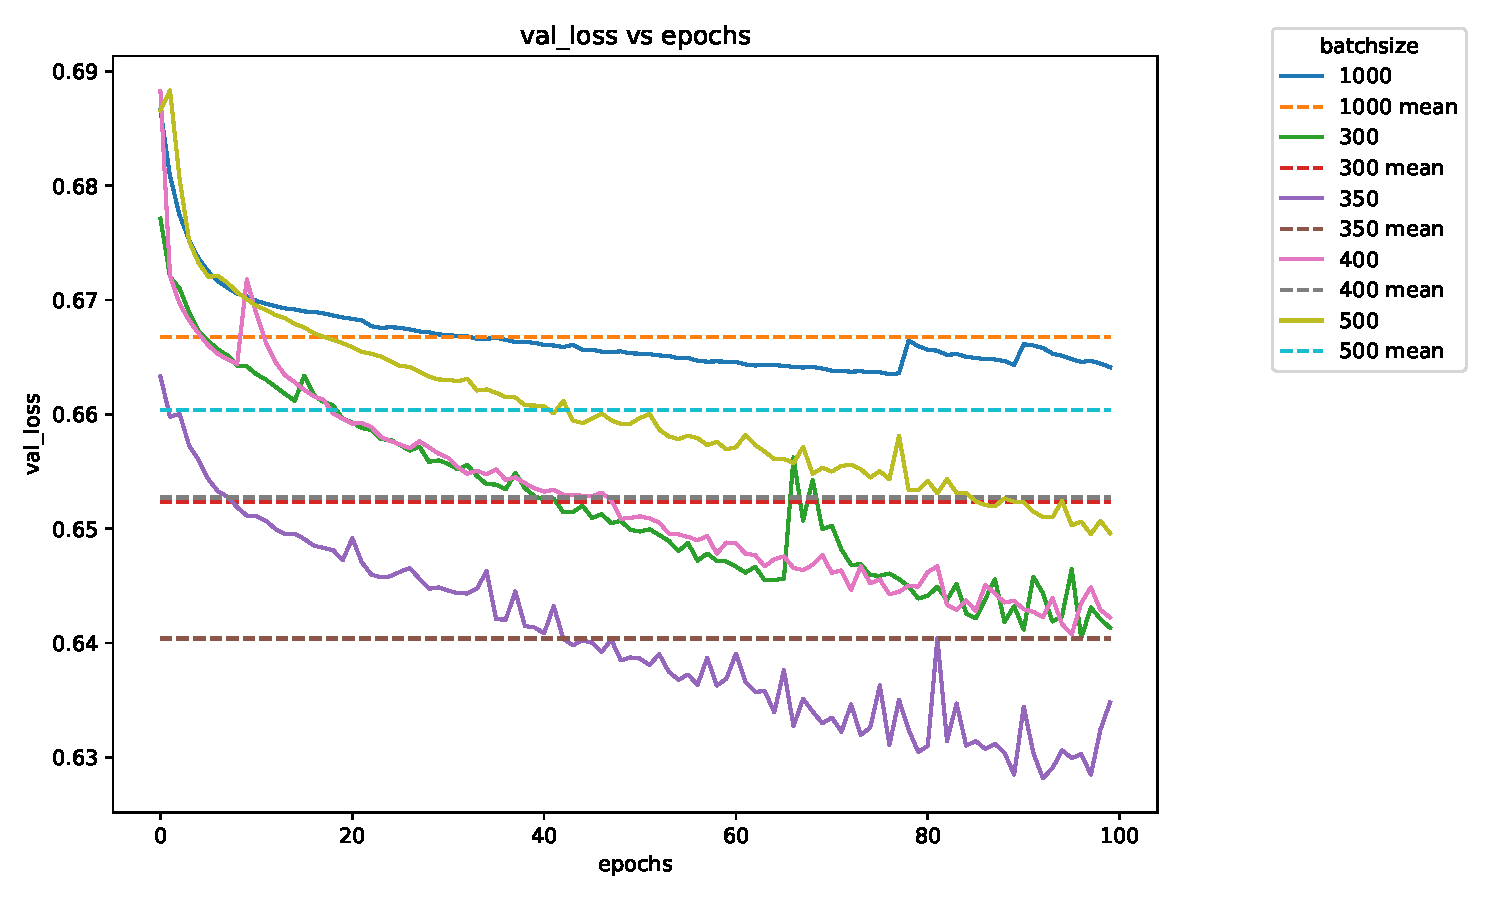
\includegraphics[width=.95\textwidth]{batchsize_val_loss.pdf}
    \caption{Comparison of both validation accuracy and loss between batchsizes.
    Our model with 2 LSTM layers, and 64 units per layer was trained over 100 epochs with the \textbf{9 errors} dataset.}
    \label{fig:batchsize}
\end{figure}

\begin{figure}
    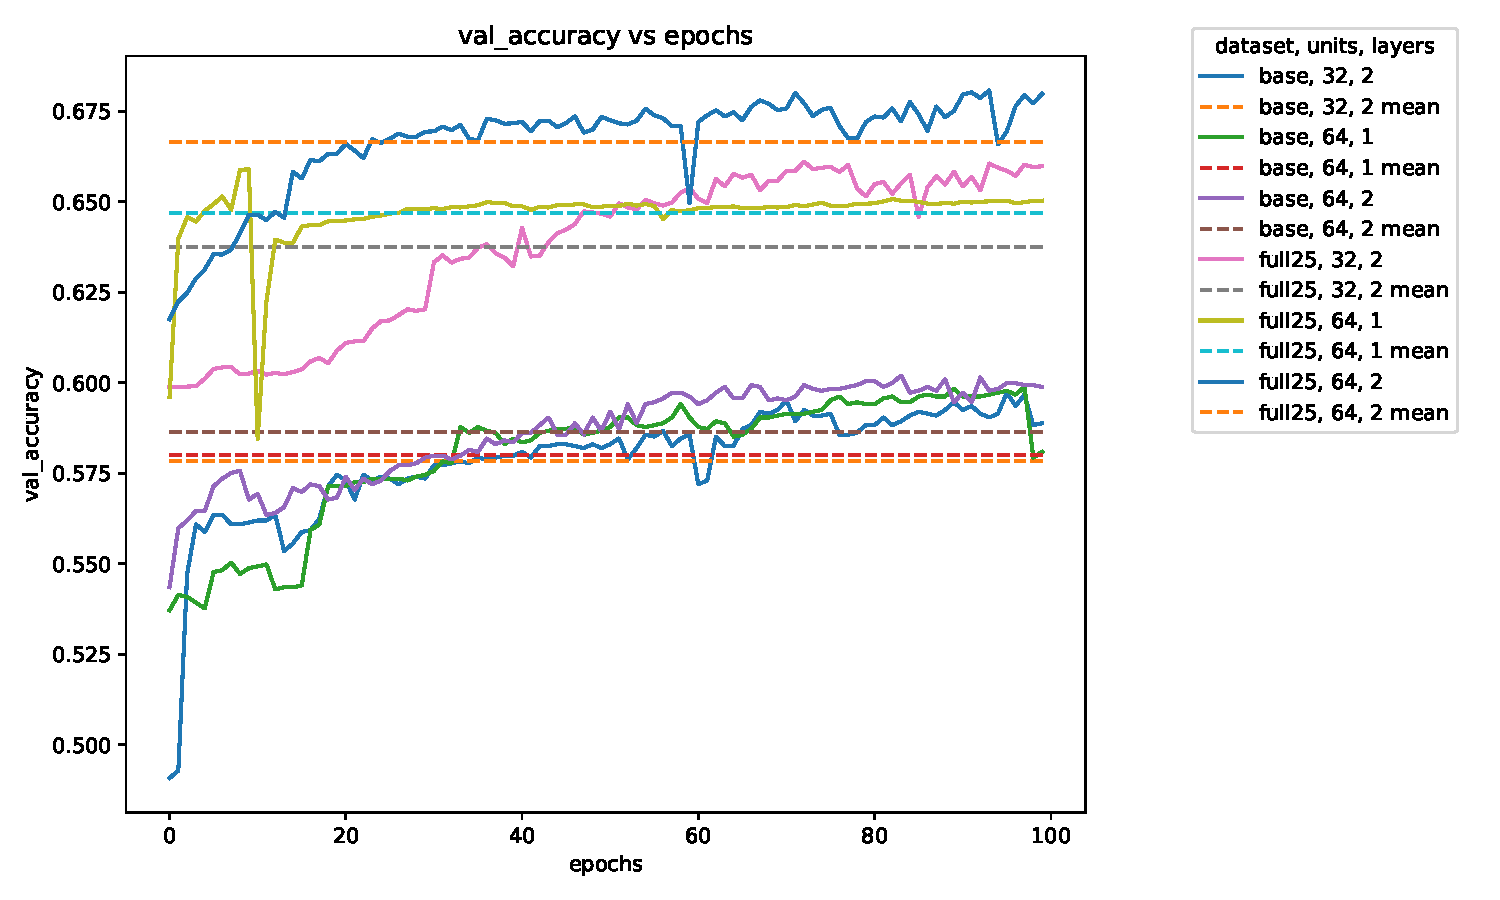
\includegraphics[width=.95\textwidth]{dataset_percentage_val_accuracy.pdf}
    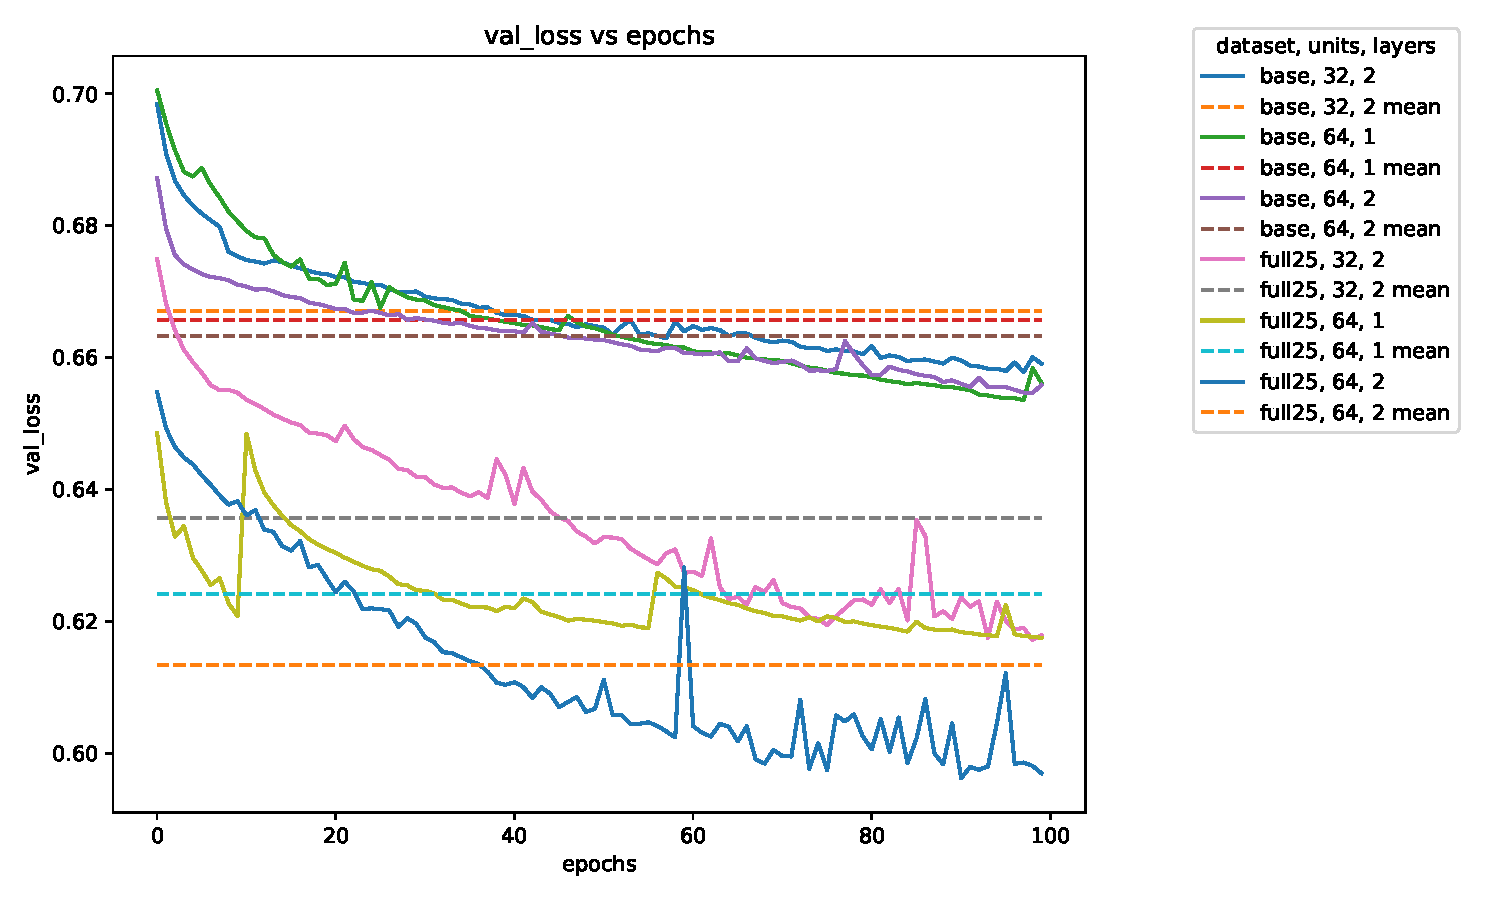
\includegraphics[width=.95\textwidth]{dataset_percentage_val_loss.pdf}
    \caption{Comparison of both validation accuracy and loss between datasets \textbf{base} and \textbf{full25}.
    Our model with various combinations of number of layers and units was trained over 100 epochs with a batchsize of 500 and the \textbf{base} dataset.}
    \label{fig:dataset_percentage}
\end{figure}

\begin{figure}
    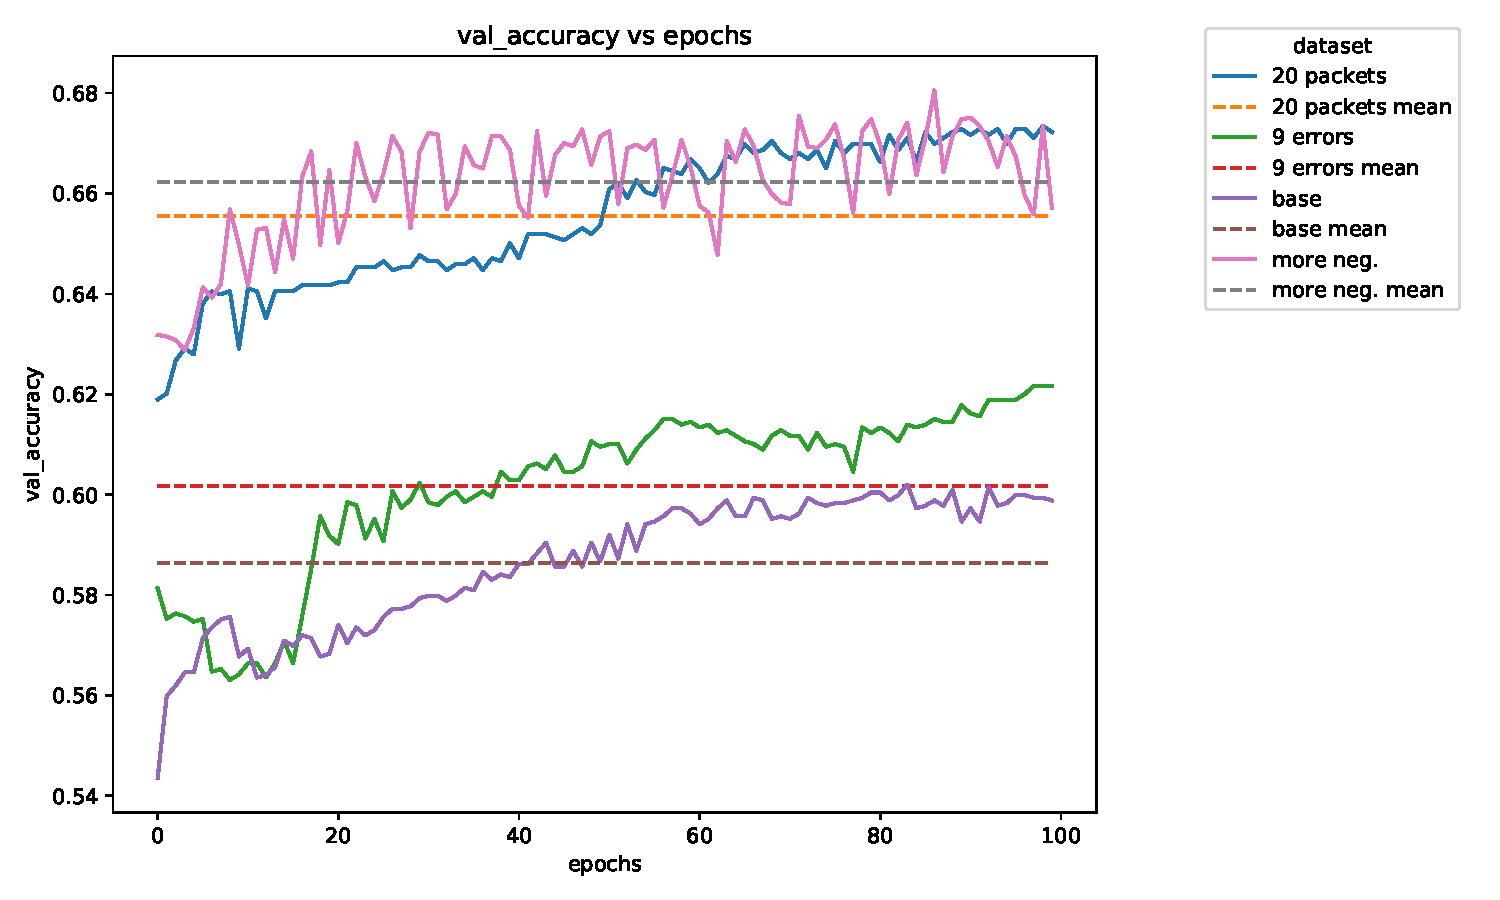
\includegraphics[width=.95\textwidth]{dataset_negative_samples_val_accuracy.pdf}
    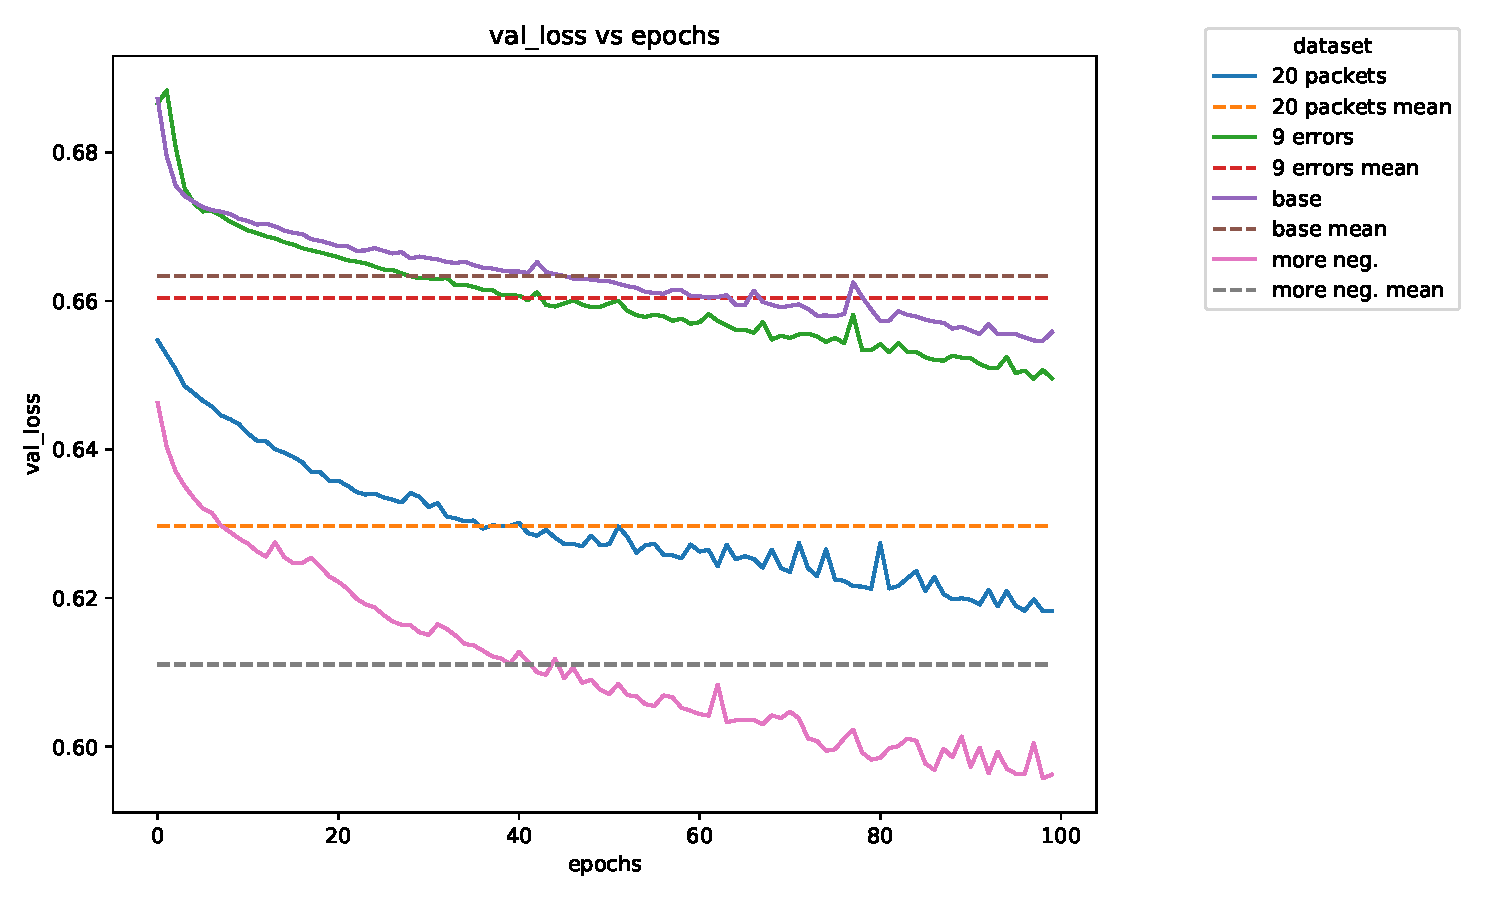
\includegraphics[width=.95\textwidth]{dataset_negative_samples_val_loss.pdf}
    \caption{Comparison of both validation accuracy and loss between datasets with various negative sample configurations, see \ref{tab:negativeSamples}.
    Our model with 2 LSTM layers, and 64 units per layer was trained over 100 epochs with a batchsize of 500.}
    \label{fig:dataset_negative}
\end{figure}

\begin{figure}
    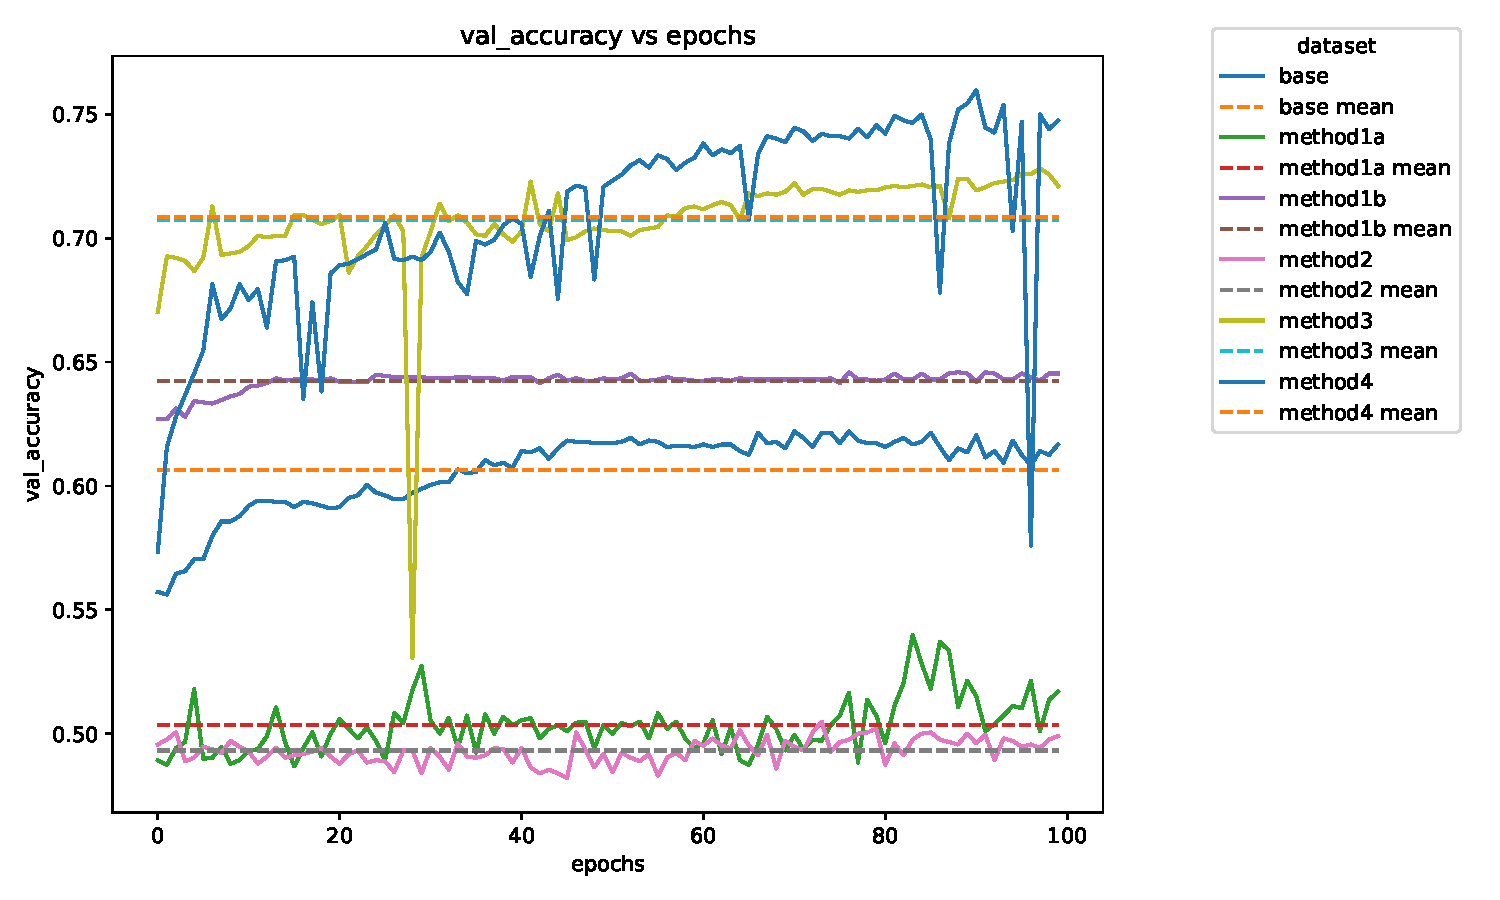
\includegraphics[width=.95\textwidth]{negative_sample_methods_val_accuracy.pdf}
    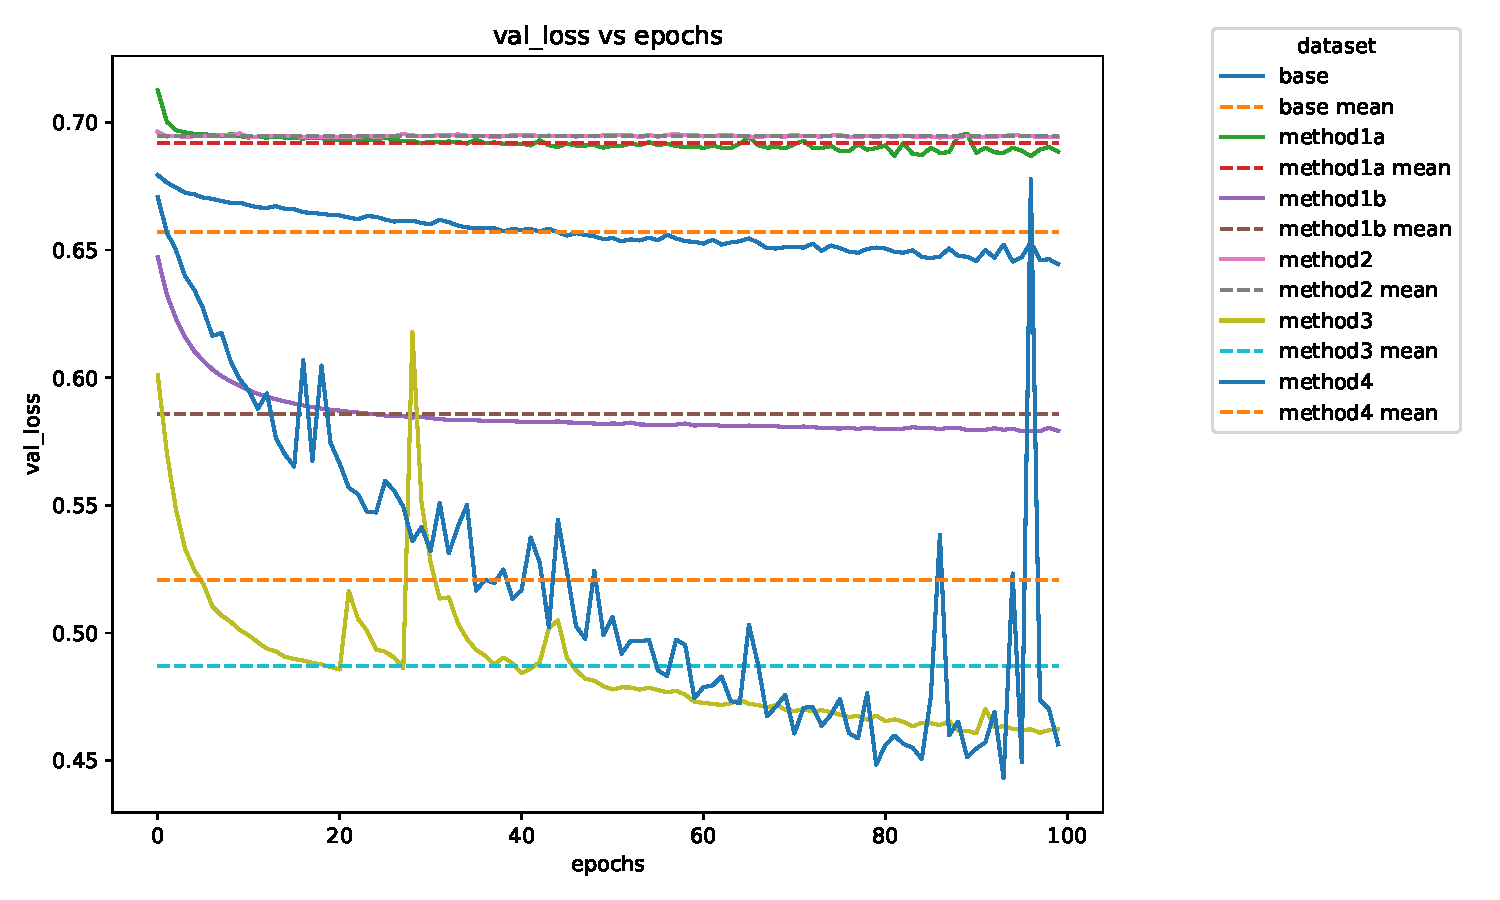
\includegraphics[width=.95\textwidth]{negative_sample_methods_val_loss.pdf}
    \caption{Comparison of both validation accuracy and loss between datasets created with only one method of negative sample creation.
    Our model with 2 LSTM layers, and 96 units per layer was trained over 100 epochs with a batchsize of 350.}
    \label{fig:negative_methods}
\end{figure}

\begin{figure}
    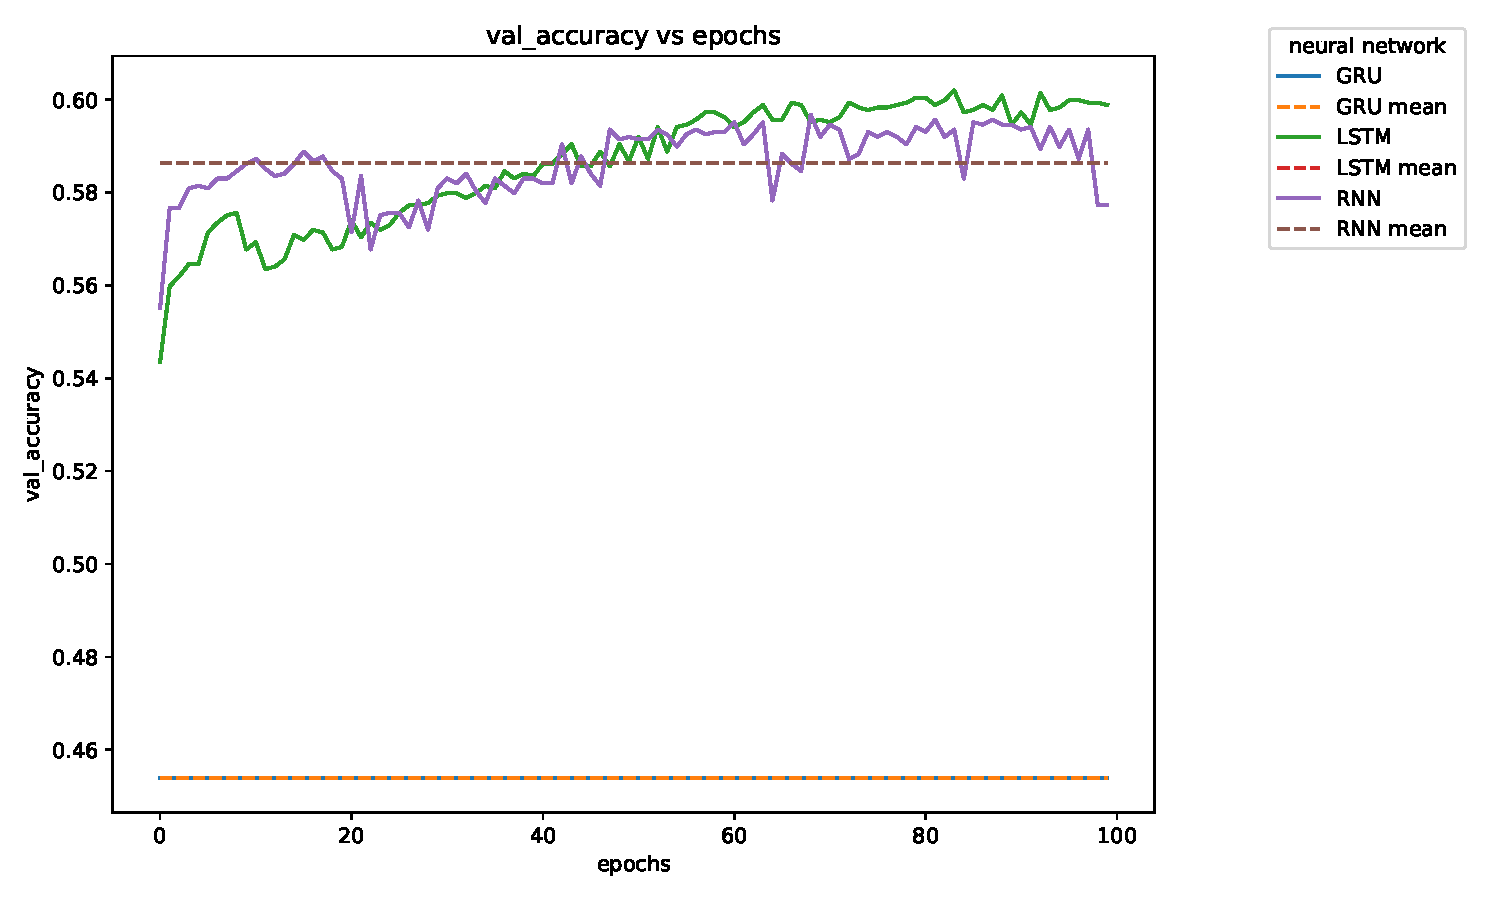
\includegraphics[width=.95\textwidth]{rnns_val_accuracy.pdf}
    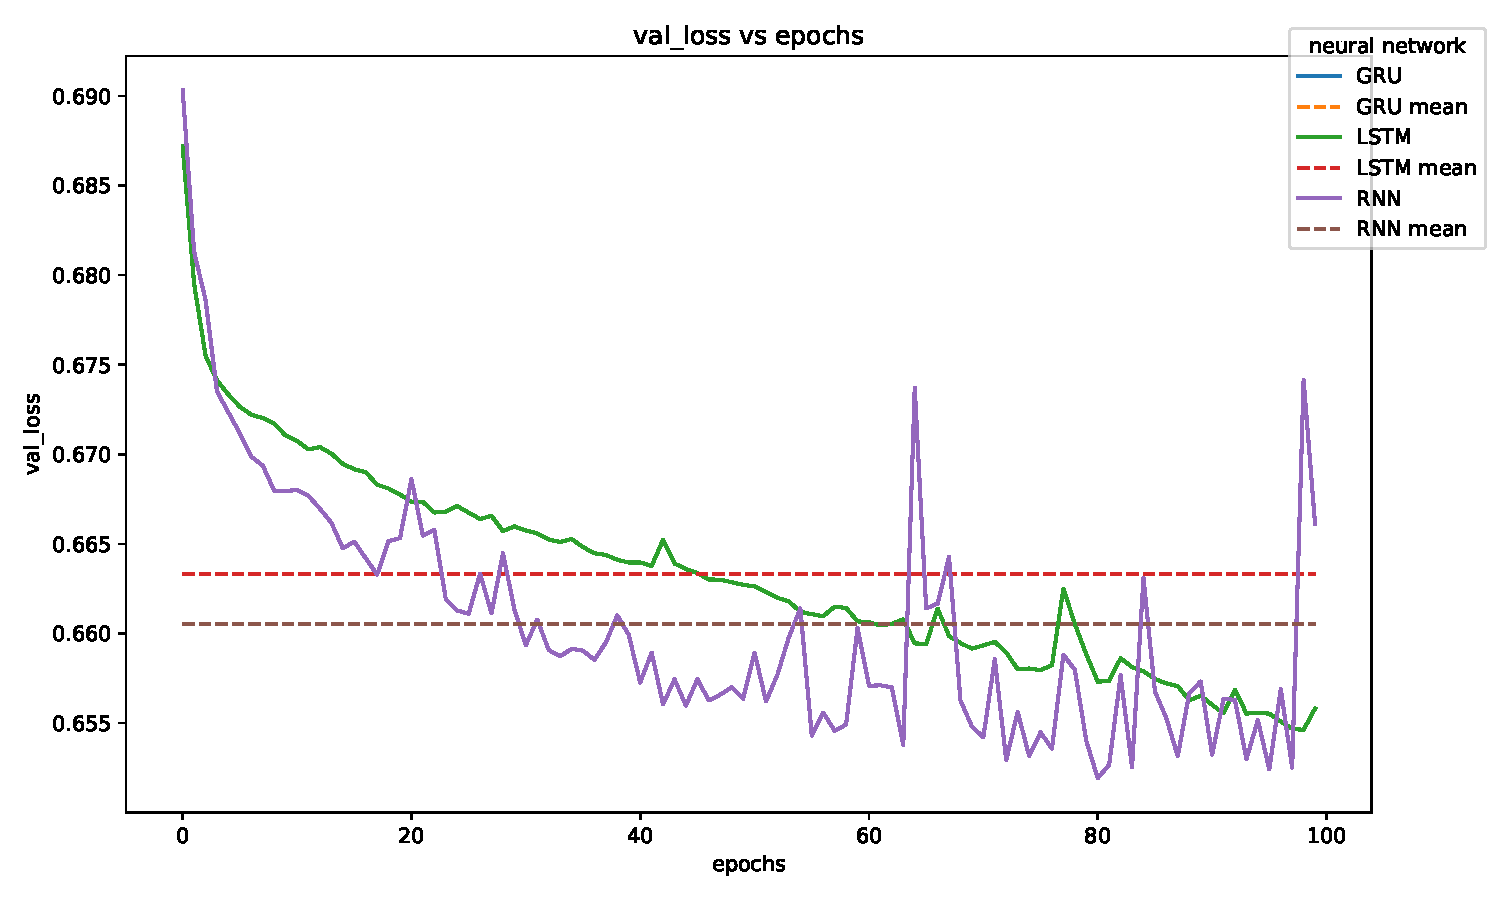
\includegraphics[width=.95\textwidth]{rnns_val_loss.pdf}
    \caption{Comparison of both validation accuracy and loss between simpleRNN, LSTM and GRU using 2 condRNN layers, 64 units per layer, and a batchsize of 500 over 100 epochs with the \textbf{base} dataset.}
    \label{fig:rnns}
\end{figure}

\begin{figure}
    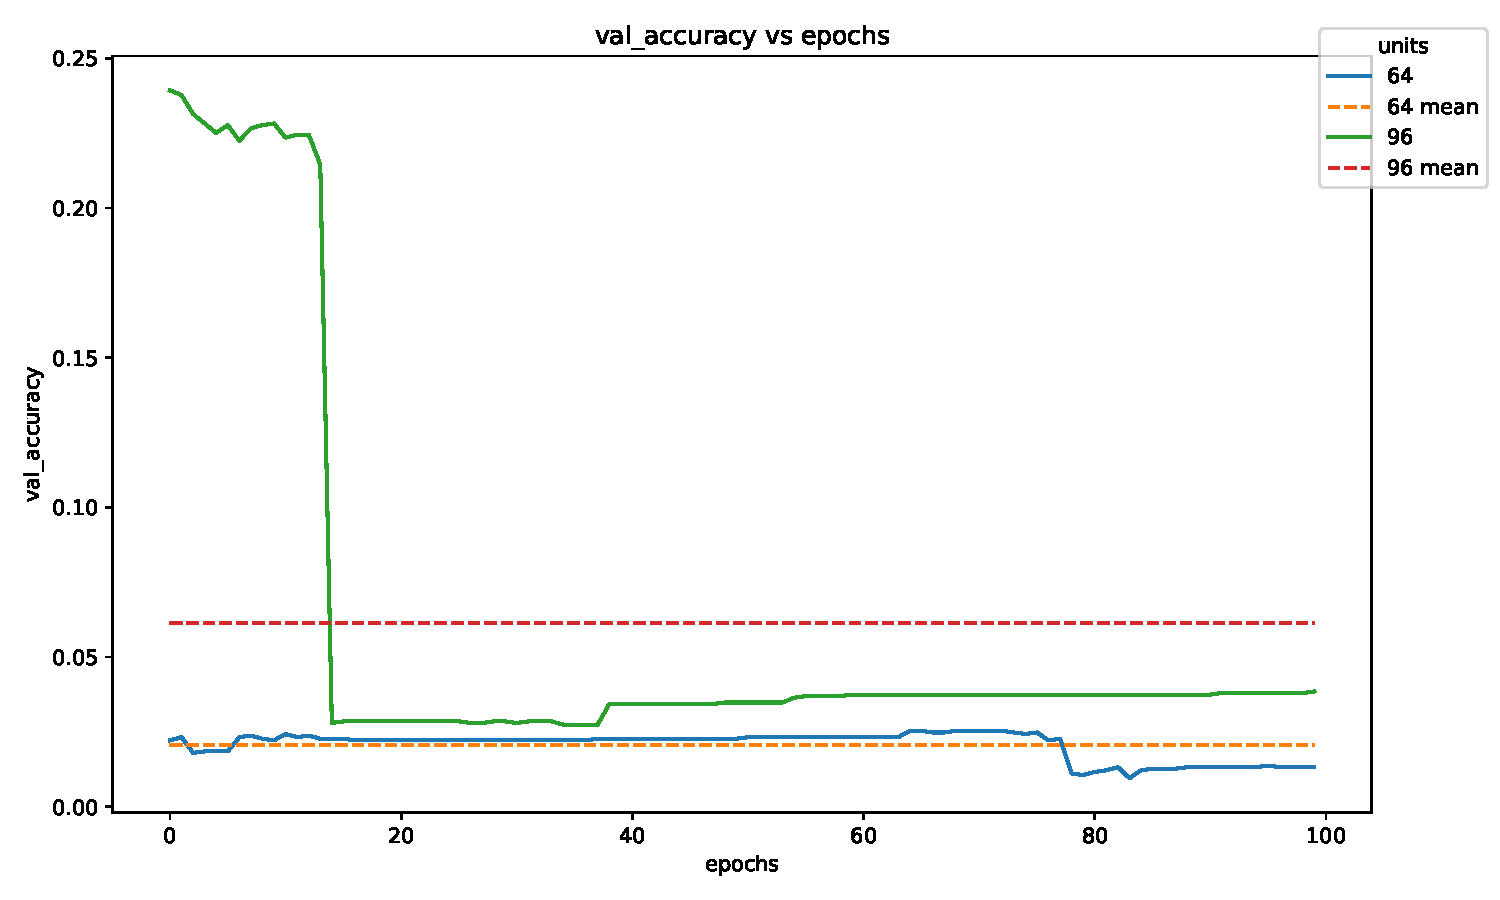
\includegraphics[width=.95\textwidth]{gru_hinge_val_accuracy.pdf}
    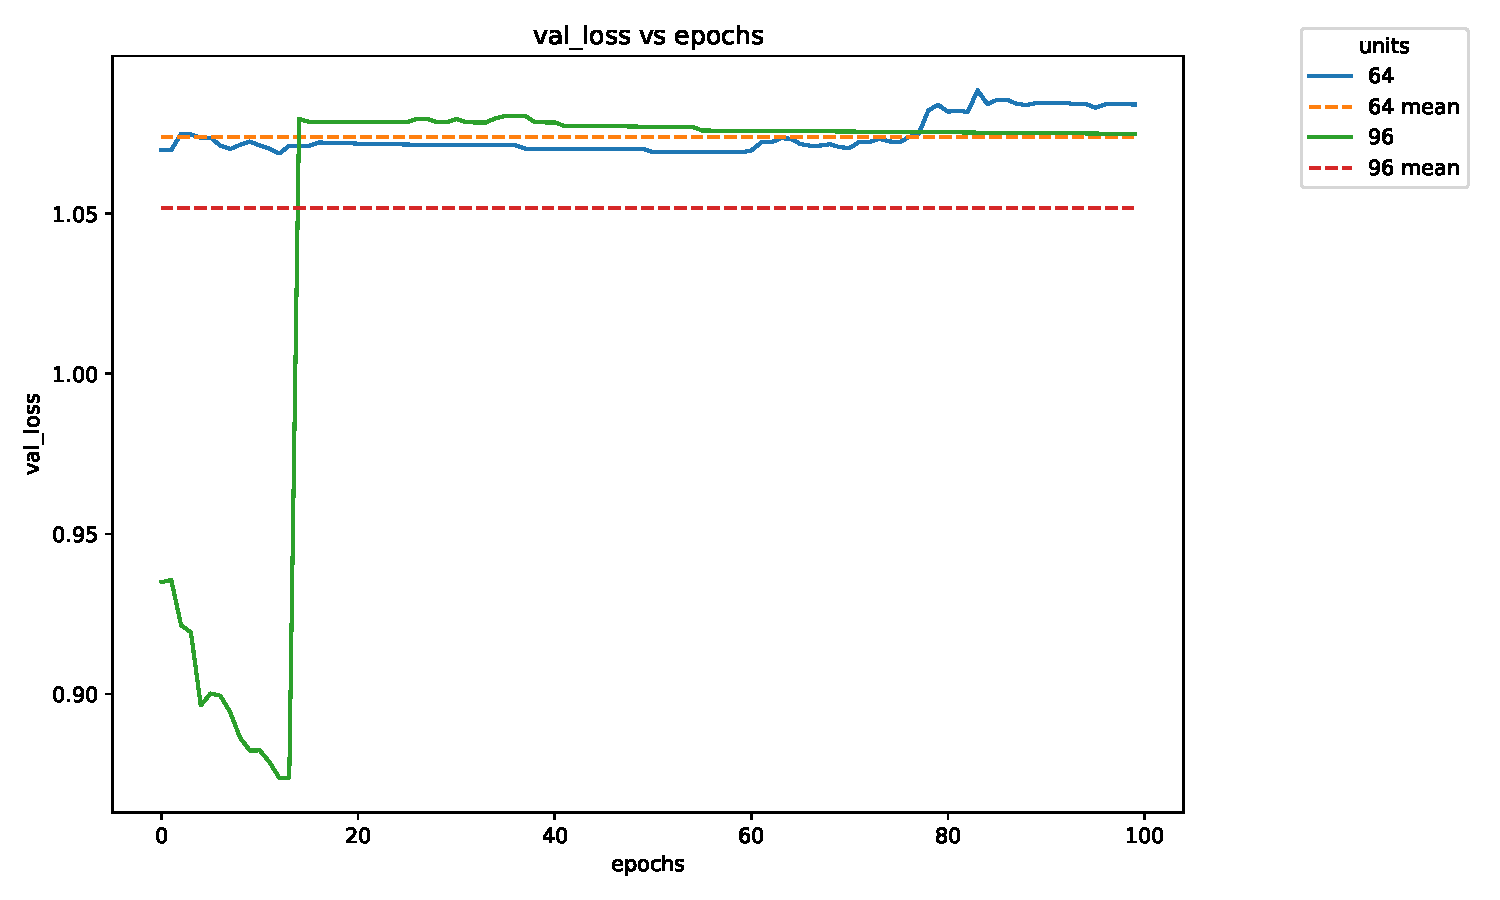
\includegraphics[width=.95\textwidth]{gru_hinge_val_loss.pdf}
    \caption{Comparison of both validation accuracy and loss between 64 and 96 units per layer.
             For this our model was trained with 1 layer of GRU units, the batchsize of 500 over 100 epochs with the \textbf{base} dataset.}
    \label{fig:GRUhinge}
\end{figure}

% \begin{figure}
%     \includegraphics[width=.95\textwidth]{}
%     \includegraphics[width=.95\textwidth]{}
%     \caption{Comparison of both validation accuracy and loss between x and y.} %TODO: parameters used
%     \label{fig:xy}
% \end{figure}

\chapter{Conclusion}
\label{sec:conclusion}

% TODO: answer the following question
% "what can you do now, what you couldn't do before?"

\section{Summary}
\label{sec:summary}

We discussed the features of packets and flows and their importance to the flow behavior and therefore to a classifier.
We created a pipeline that creates datasets, where each datapoint is a pair of a network flow and a network packet sequence, for use with NNs.
Said pipeline is capable of sampling random flows from network packet captures, extracting flow and packet features and creating negative datapoints.
% FIXME: no we did not
We provided a proof of concept classifier that can distinguish if a flow could have been created by a sequence of packets.
This NN model could be used as a DN for a GAN that creates network packet sequences from a network flow.
% FIXME: it is still possible that LSTMs are the way to go, however we did not show nor conclude that!
We also evaluated the effectiveness of different RNN architectures for this task
and concluded that LSTMs are best suited for it.
Additionally we researched how to handle non-static input for RNNs and provided an implementation based on conditional RNN layers.

\section{Research Contributions}
\label{sec:Contributions}

% FIXME: we did not provide a proof of concept!
Even though the results were not optimal this work provides a proof of concept RNN model that is capable of distinguishing if a network flow could have been created by a sequence of network packets.
However this is not the main contribution.
The most valuable research contribution would be the discussion on network packet and flow features we take into account, as well as the derivation of the data.
Furthermore we will publish the pipeline for effectively sampling network packet captures and created negative samples, so that future research can benefit from it.

\subsection{Answering the Research Questions}
\label{sec:answers}

\paragraph{How can we develop a neural network that acts as a discriminator for a GAN that can determine if a network flow could have been created by a sequence of network packets?}
Most likely yes.
Our NN model is capable of discriminating if a network flow was created by a sequence of network packets.
It should be able to be used as a DN for the proposed GAN.

\paragraph{Which features of network flows and packets are (most) significant to determine if a network flow could have been created by a sequence of network packets?}
This question was answered in-depth in section \ref{sec:datapointFeatures}.

\paragraph{Which NN architecture would be most suitable to distinguish if network packets could have created some network flow?}
Based on our experiments LSTMs provide the best results, specifically conditional LSTMs (condLTMs).

\section{Future Work}
\label{sec:futureWork}

This work sets the groundstone for a variety of future work.
Most of all the GAN proposed in the introduction.

\subsection{Generation of network traffic captures with GANs}
\label{sec:futureGAN}

As stated many times throughout this thesis, we created a NN that can serve as a DN for a GAN that creates synthetic and authentic network packets from a network flow.
The next step for this would be implement a GN that can be used in combination with our DN.
It is also advised to gather more data to be more representative of the real world.
The dataset we created is limited by its source data, which was fine for a proof of concept, but will not be sufficient when applied to real-world problems.

\subsection{Federated Learning}
\label{sec:FL}

Once the GAN proposed above produces good results, one could combine it with federated learning (FL).
% explain FL
In the last couple of years, FL has become a widely used method to protect user data while training ML models.
So one real-world application for the GAN could be to deploy it with NIDSs, routers of big ISPs, or the routers of personal users.
This way, the GAN could be trained with real-world traffic without compromising the privacy of the data.
The paper "FedGAN: Federated Generative Adversarial Networks for Distributed Data" by Rasouli et al. \cite{rasouliFedGANFederatedGenerative2020} introduces a federated GAN (FedGAN) that uses local generators and discriminators.
This way, multiple users could add their traffic datasets without exposing their data.

FL in general still has flaws regarding privacy, but multiple researchers are working on improving the privacy of FL for example, in the form of differential privacy (DP).
DP tries to preserve the user's privacy by compromising accuracy.
The most common methods to achieve DP are clipping the weights, which will be send to the server, and the addition of noise before averaging weights in order to anonymize the single contributions and minimize the information about the user that is extractable.
Some libraries, e.g. PySyft, also provide homomorphic encryption, so the end-user might not have to train on their data themselves.
Instead, they could send the encrypted data to an intermediate server, which computes the model with the encrypted data.
Therefore also never seeing the data itself, while the computation heavy part is not done locally.
This is specifically interesting if we consider using a FedGAN to train on data collected by consumer routers,
as those usually do not have much computation power to begin with.

With a GAN that also respects appropriately labeled intrusion detection network captures,
combining this approach with FL could have the potential to solve the issue of creating synthetic network traffic for self learning anomaly based NIDSs.

\subsection{Possible Model Adjustments}
\label{sec:modelAdj}

As described already in the thesis a condRNN uses the conditional input to initiate the state of the RNN layer before the seqeuntial input gets processed.
This behavior was appropriate to the task of image description generation \cite{vinyalsShowTellNeural2015} \cite{karpathyDeepVisualSemanticAlignments2015} as the sequence data only consisted of one or two sentences.
At most those were 50 words long.
Even with word2vec this would most likely never be as much as the data we used.
Our sequential data is only limited to 500 packets and each packet has around 66 features.
It is possible that the RNN has forgotten all the flow information from the conditional input by the time it reaches the end of the sequence.
One could propose an advanced condRNN that feeds the conditional input into the state every X number of timestamps or even with every timestamp of the sequence.
In the future we might explore this and look into how it affects the results of our NN model.

Our NN handling both the UDP and the TCP protocol allows us to have negative samples, in which the transport protocol was changed.
We view this as a benefit of our design, as it also would also allows the future additions of other protocols.
However in future work it might be interesting to compare our results to a NN model that consists of two RNNs, where one is handling UDP and one is handling TCP packet sequences.

\subsection{Feature Improvements}
\label{sec:featureImprovements}

As this thesis was a proof of concept for a NN that is capable of discriminating if a network flow could have been created from a given sequence of network packets, it leaves some opportunity for future work regarding improvements or optimizations.
Besides improvements to the NN model additions or removal of packet and flow features might yield interesting results.
We see three categories where the work could be improved.
Tailoring an IP2Vec approach for MAC addresses, IPs and ports. ...
Especially in conjunction with FL.
Adding the trivial features as binary representation (valid/invalid).
Brining in more meta data extracted from statistics or general network flow behavior.

Also interesting if other network flow representations yield the same results.

% TODO: talk about dead features - (last two) end reasons

\printbibliography

\end{document}
